\chapter{Estimación de los fondos} \label{cap:fondos}

Como se describe en el \cref{sec:signal_regions}, utilizando las
muestras MC, se estima que la contribución dominante de fondos del Modelo
Estándar es la producción de {\wgam} y {\ttgam}. Además en la {\SRL} también se
espera una contribución de procesos de {\ttbar} en los que un electrón es mal
identificado como fotón.

En este capítulo se describe la estrategia utilizada para la estimación de los
fondos contaminantes provenientes de procesos del SM.
%% En elcaso de que estos
%% no puedan ser calculados a partir de simulaciones MC debido a que los modelos
%% son incompletos
Los fondos provenientes de electrones o jets mal identificados como fotones son
estimados a partir los datos observados como se describe en las
\cref{sec:efakes,sec:jfakes}, respectivamente. %%\note{Revisar parrafo}.
Para los fondos más importantes, {\wgam} y
{\ttgam}, como no es posible obtener una estimación de los datos, se
utilizan las muestras simuladas por MC pero corregidas usando los datos en
una región de control, como se explica en la \cref{sec:bkg_wgam_ttgam}. La
misma técnica se utiliza para el fondo de {\gjet} que, a pesar de ser
despreciable en las SR, si la energía faltante producida por la mala
reconstrucción de los jets es elevada, puede ser relevante (ver
\cref{sec:bkg_gjet}). Las demás contribuciones, que son despreciables en
las regiones de señal, se estimaron directamente de las muestras MC.

%% El fondo de {\gjet} no es un fondo importante en las SR debido a que no posee energía faltante
%% verdadera y por lo tanto el corte en {\met} es suficiente para reducirlo significativamente.
%% A pesar de eso, como las simulaciones Monte Carlo ... también se utiliza una CR para
%% corregir la normalización de la misma.


\section[Producción de {\wgam} y $tt\gamma$]{Producción de {\wgam} y {\ttgam}}
\label{sec:bkg_wgam_ttgam}

Los eventos provenientes de la producción de {\wgam} y {\ttgam} son las
contribuciones dominantes al fondo en ambas regiones de señal.

La producción de {\wgam} dominante es básicamente $pp \to W\gamma + X \to \nu_l
\bar{l}\gamma + X$. Cuando el leptón no es reconstruido o se pierde por la
aceptancia del detector, pueden entrar en la SR. En el caso que el $W$
decaiga hadrónicamente no hay energía faltante y se espera de simulaciones MC que
su contribución sea despreciable. Para la estimación final se considera
esta contribución a partir de las muestras MC ($V(\to qq)\gamma$).

En el caso de {\ttgam}, cada quark \emph{top} decae en un bosón $W$ y un
{\bjet}. Si uno de los $W$ decae leptónicamente y el leptón no es identificado
ocurre lo mismo que en el caso de {\wgam} y puede contaminar la SR.

Se definen entonces dos regiones de control para determinar la normalización del
MC de {\wgam} (CRW) y {\ttgam} (CRT). Cada una de estas regiones de control es
diseñada para que esté dominada por cada uno de estos fondos, para lo cual se
pide un fotón, un leptón, jets y \met. Para {\CRW} se pide además que no haya
{\bjets} en el evento para reducir la contaminación de {\ttgam}, mientras que
para {\CRT} se requiere la presencia de al menos uno.
Los cortes de selección se mantienen lo
más similares posibles a la correspondiente SR para minimizar el efecto de la
extrapolación, mientras que se remueven o relajan
algunos cortes para aumentar la estadística. En especial, se relaja el corte en
{\met} y no se aplican los cortes en {\HT} y en {\rt}. Un esquema muy simple de
estas CR puede verse en \cref{fig:bkg_crt_crw}.

La selección completa de cada CR se presenta en la \cref{tab:bkg_crs}. Se utilizan
dos regiones de control asociadas a cada SR.

\begin{figure}[!htbp]
  \centering

  \resizebox{0.5\textwidth}{!}{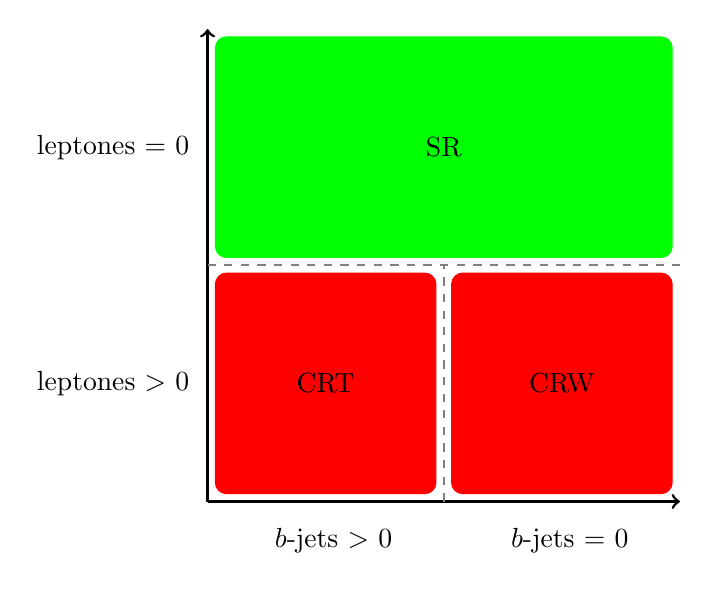
\begin{tikzpicture}[domain=0:4]

  \tikzstyle{region} = [rounded corners, fill]

  \draw[line width=1, ->] (0,0) -- (6,0);
  \draw[line width=1, ->] (0,0) -- (0,6);

  \draw[gray, dashed, line width=0.8] (0, 3.0) -- (6.0, 3.0);
  \draw[gray, dashed, line width=0.8] (3.0, 0) -- (3.0, 3.0);

  \draw node at (1.6,-0.5) {$b$-jets $>$ 0};
  \draw node at (4.6,-0.5) {$b$-jets = 0};
  \draw node at (-1.2, 1.5) {leptones $>$ 0};
  \draw node at (-1.2, 4.5) {leptones = 0};

  \draw[green, region] (0.1,3.1) rectangle (5.9,5.9);
  \draw node at (3.0,4.5) {SR};

  \draw[red, region] (0.1,0.1) rectangle (2.9,2.9) ;
  \draw node at (1.5,1.5) {CRT};

  \draw[red, region] (3.1,0.1) rectangle (5.9,2.9) ;
  \draw node at (4.5,1.5) {CRW};

\end{tikzpicture}
}

  \caption{Regiones de control definidas para normalizar el fondo de {\wgam} (CRW) y {\ttgam} (CRT). En este contexto <<leptón>> se refiere solo a electrones o muones.}
  \label{fig:bkg_crt_crw}
\end{figure}



\begin{table}[!htbp]
  \centering

  \caption{Selección para las regiones de control utilizadas para normalizar los
    fondos de {\wgam}, {\ttgam} y {\gjet}, asociadas a las regiones de señal
    {\SRL} y {\SRH}}
  \label{tab:bkg_crs}

  \begin{tabularx}{\textwidth}{r|CCC|CCC}

    \hline
                                     & \multicolumn{3}{c|}{\SRL} & \multicolumn{3}{c}{\SRH} \\
    \cline{2-7}
                                     &      \CRWL &      \CRTL &  \CRQL &     \CRWH &    \CRTH  &   \CRQH \\
  \hline
  $\pt^\gamma$ [\gev] $>$            &        125 &        125 &    125 &       150 &      150  &     300 \\
  $N_\mathrm{leptones}$              &          1 &    $\ge 1$ &      0 &         1 &  $\ge 1$  &       0 \\
  {\met} [\gev]                      &  [100-200] &   [80-200] &  $<50$ &  [100-200] & [80-200] &   $<50$ \\
  $N_\mathrm{jets} \ge$              &          4 &          4 &      4 &         2 &        2  &       2 \\
  $N_{b\text{-jets}}$                &          0 &    $\ge 1$ &      - &         0 &  $\ge 1$  &       - \\
  $\pt^{j_1},\pt^{j_2}$ [\gev] $>$   &        100 &        100 &    100 &        40 &       40  &      40 \\
  $\dphijm >$                        &        0.4 &        0.4 &    0.4 &       0.4 &      0.4  &     0.4 \\
  $\rt <$                            &          - &          - &   0.85 &         - &        -  &       - \\
  {\HT} [\gev] $>$                   &          - &          - &      - &         - &        -  &   $800$ \\
  $\dphijg <$                        &          - &          - &      - &       2.0 &      2.0  &     2.0 \\
  \hline
  \end{tabularx}

\end{table}


%% As seen in \Fig \ref{fig:sig_CR}, the signal contamination in the CRs is
%% expected to be small. For CRM, the low \MET cut kills most of the signal events,
%% keeping its fraction below 0.5\% across the whole grid and decreasing with the
%% gluon mass.

%% ## CRLW_2
%% Percentage of wgamma:  63.26 % 3.81429171562 / 6.02966526151
%% Largest contamination:  41.84 %
%% ## CRLW_3
%% Percentage of wgamma:  69.18 % 15.5461444855 / 22.4714100622
%% Largest contamination:  11.3 %
%% ## CRLT_2
%% Percentage of ttbarg:  55.83 % 8.56628704071 / 15.3442126885
%% Largest contamination:  74.96 %
%% ## CRLT_3
%% Percentage of ttbarg:  60.23 % 14.3853740692 / 23.8827633113
%% Largest contamination:  40.28 %

Es importante que las CR no tengan una contaminación de señal y para tal fin se
aplica, además, un corte superior en {\met}. En {\CRW} y {\CRT} la contaminación
de señal en las CR es $<3\%$ para la mayor parte de la grid, aunque es mayor
(hasta 70\%) para algunos puntos de baja masa de gluino en {\CRTL} (ver
\cref{fig:bkg_cr_contamination}).

\begin{figure}[!htbp]
  \centering

  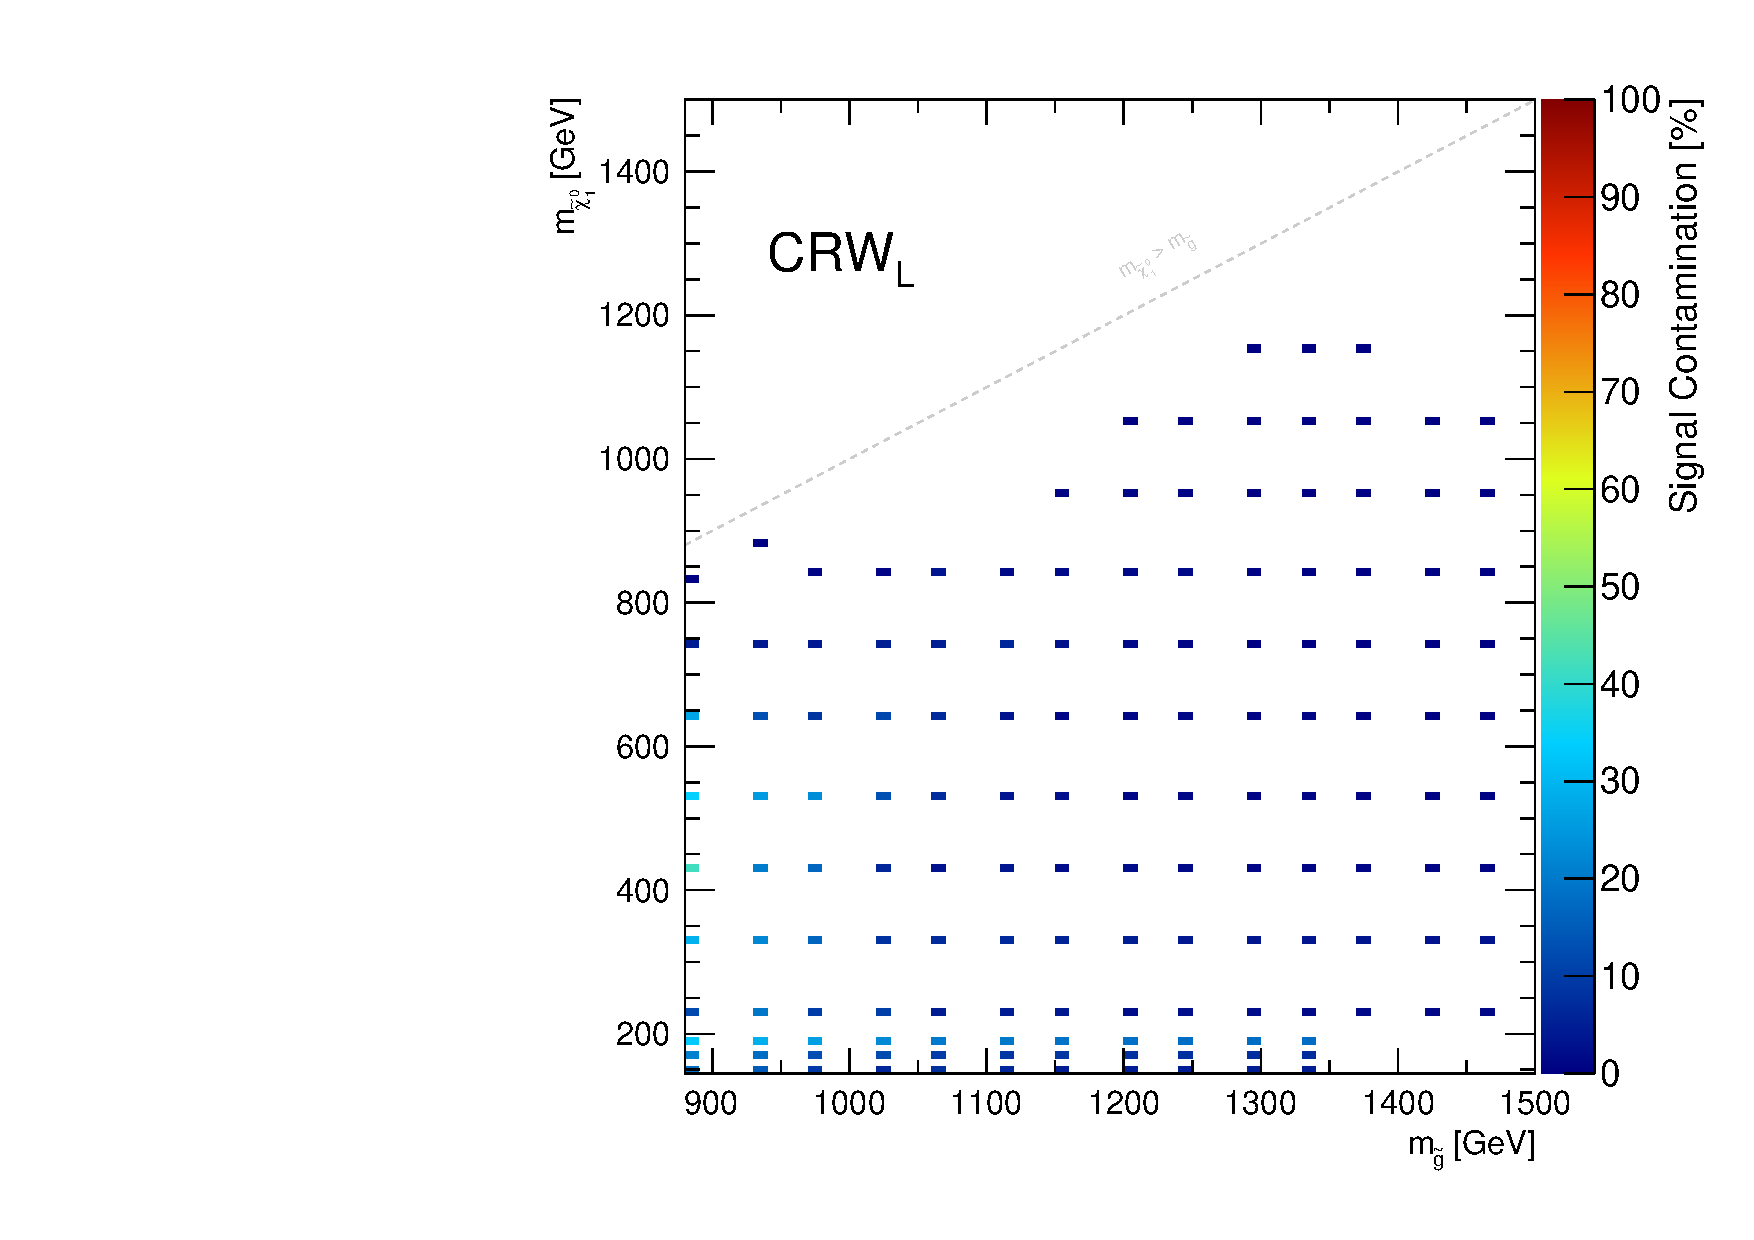
\includegraphics[width=0.46\textwidth]{signal_contamination_crwl}\hspace{1cm}
  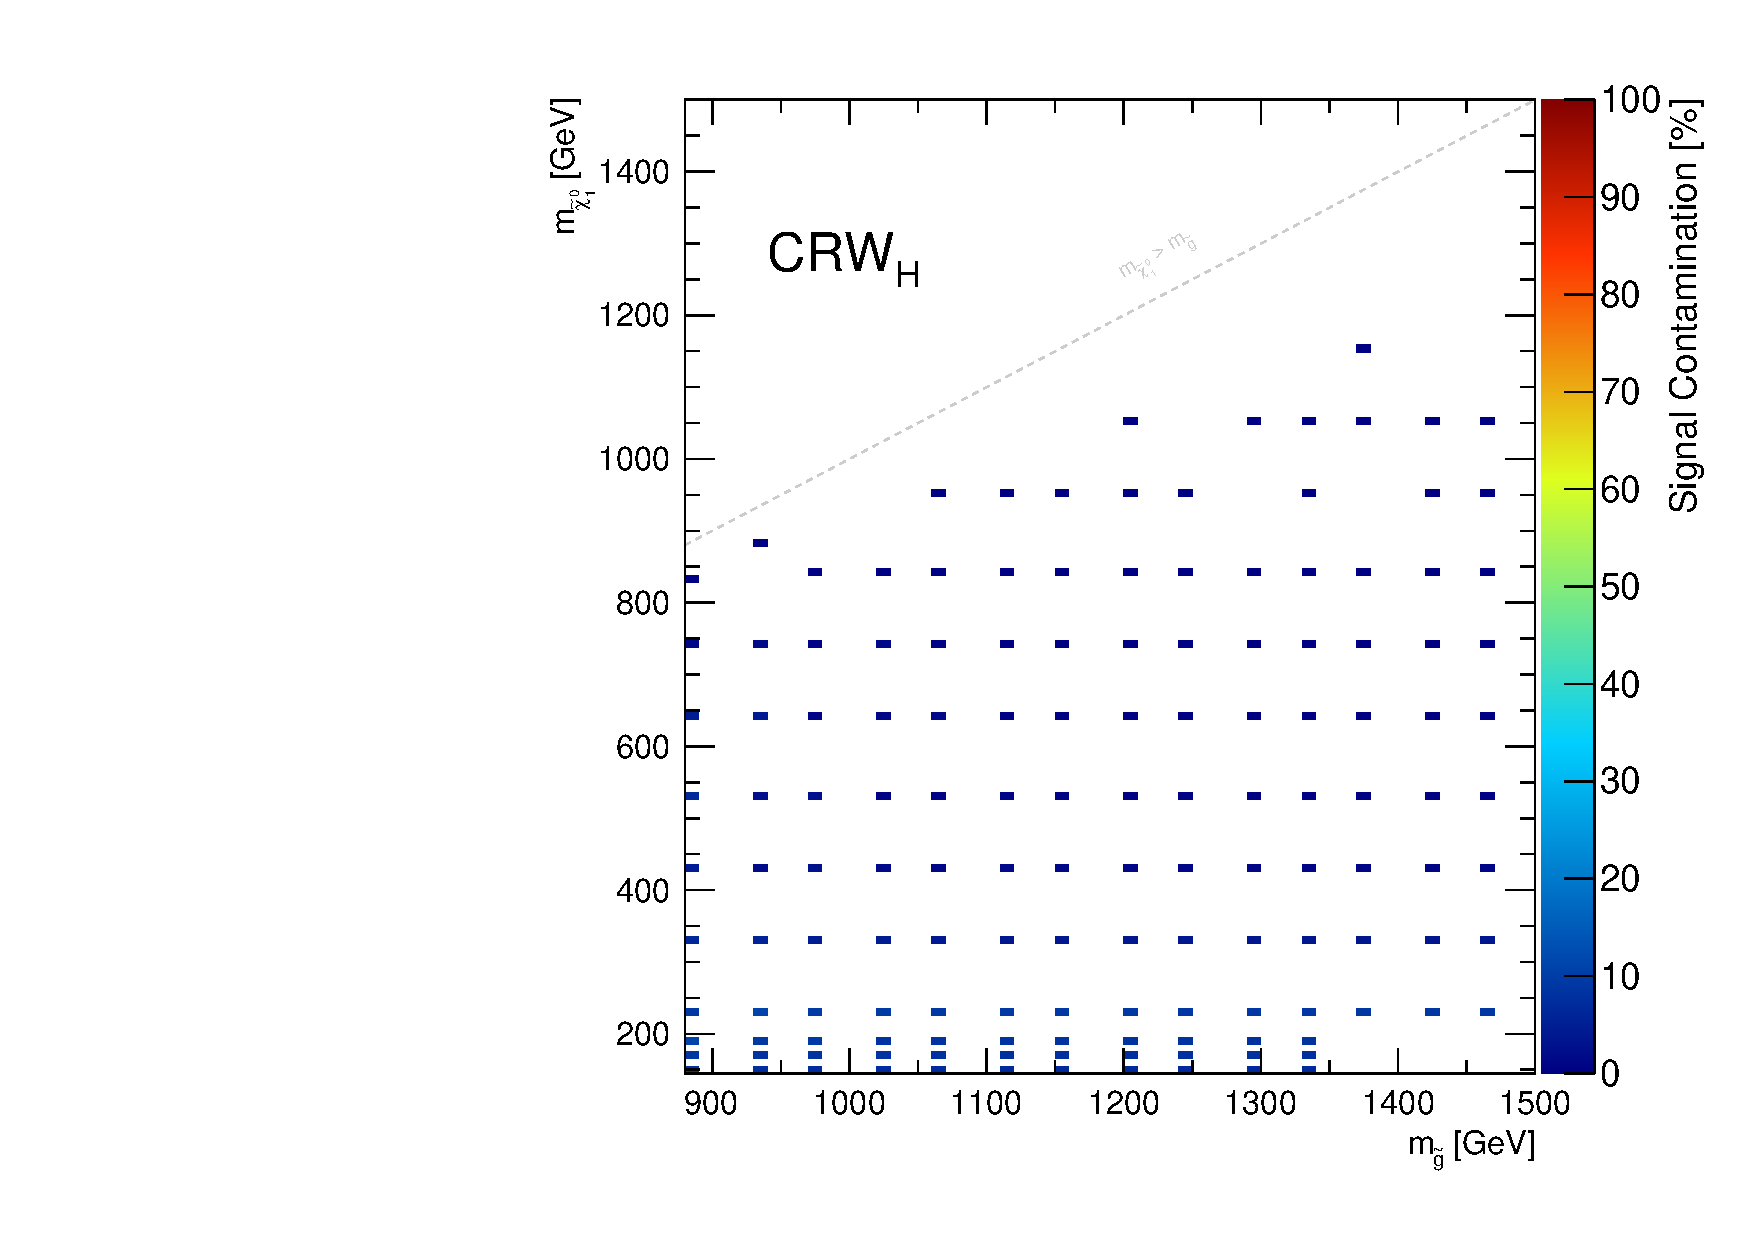
\includegraphics[width=0.46\textwidth]{signal_contamination_crwh}

  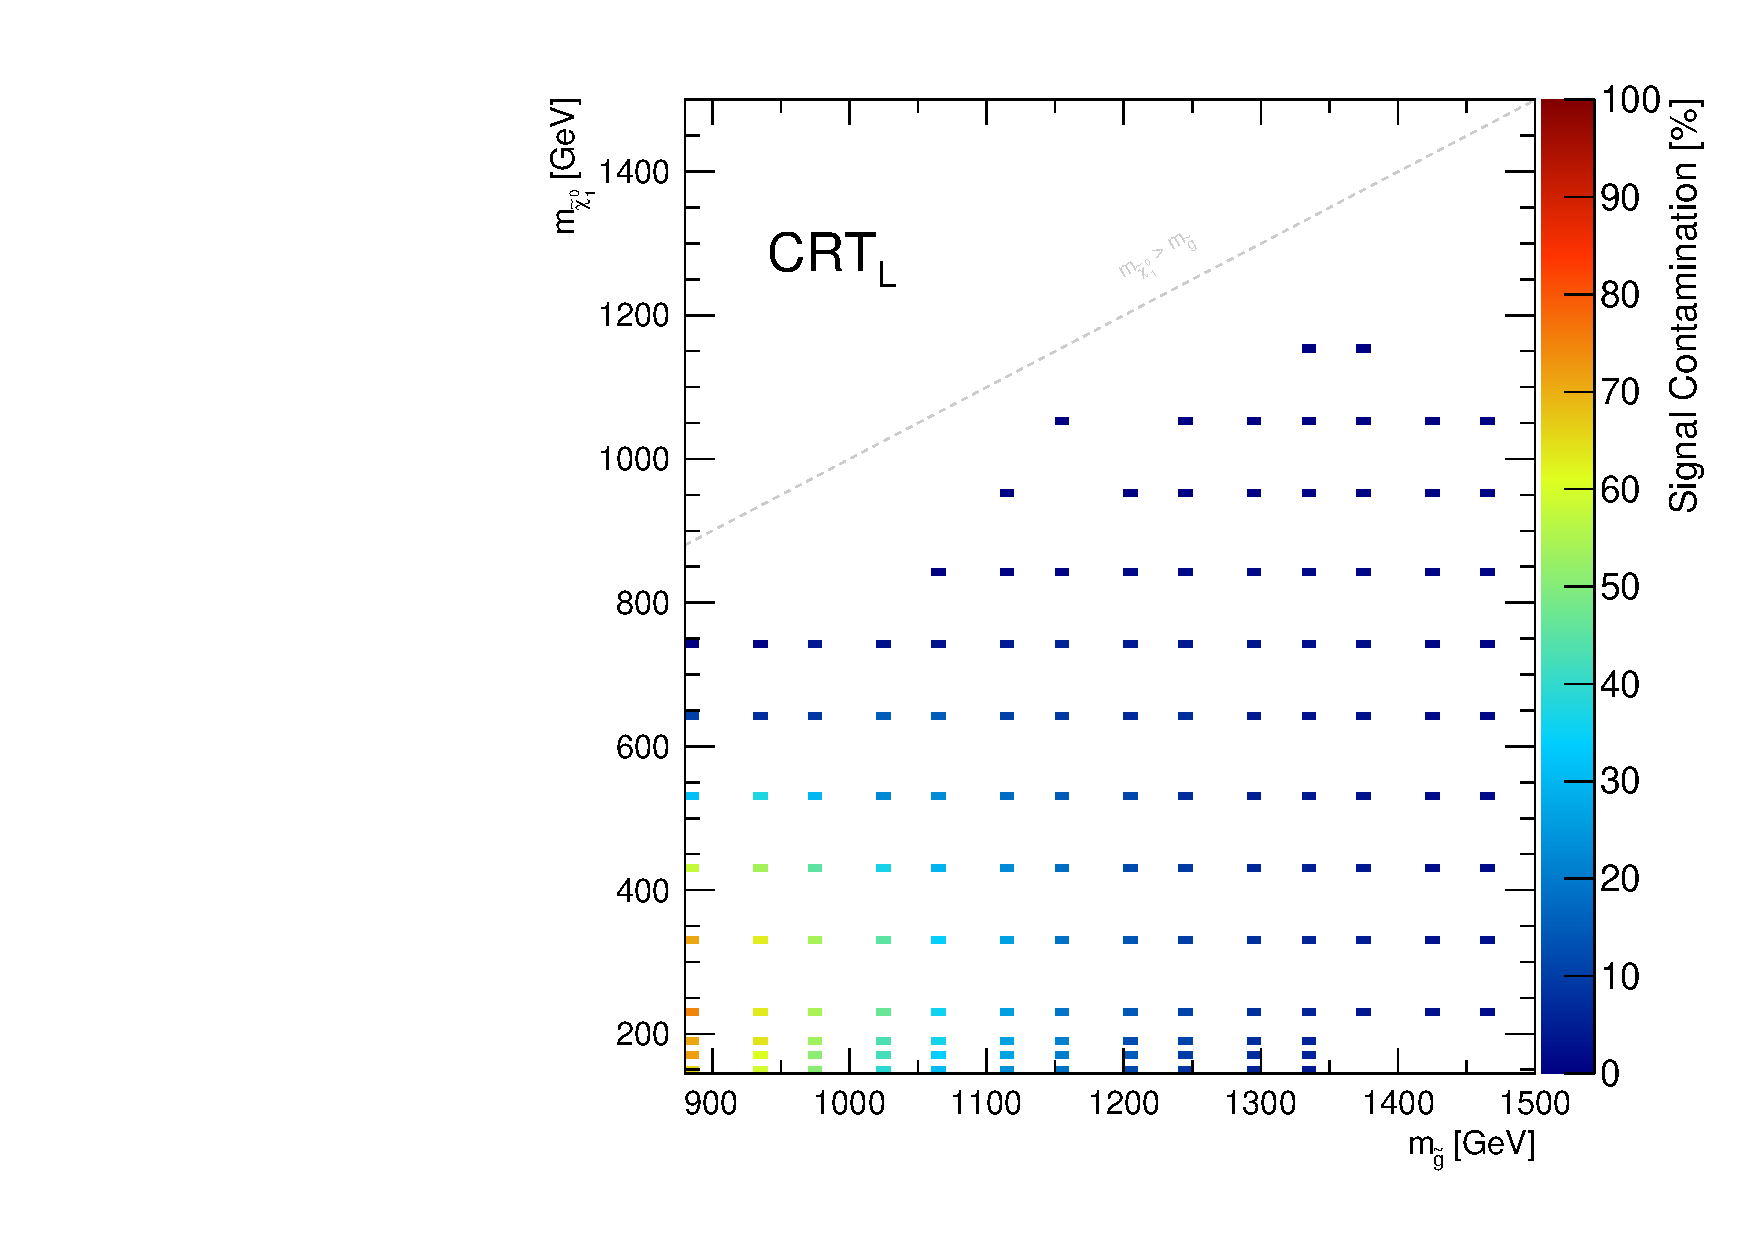
\includegraphics[width=0.46\textwidth]{signal_contamination_crtl}\hspace{1cm}
  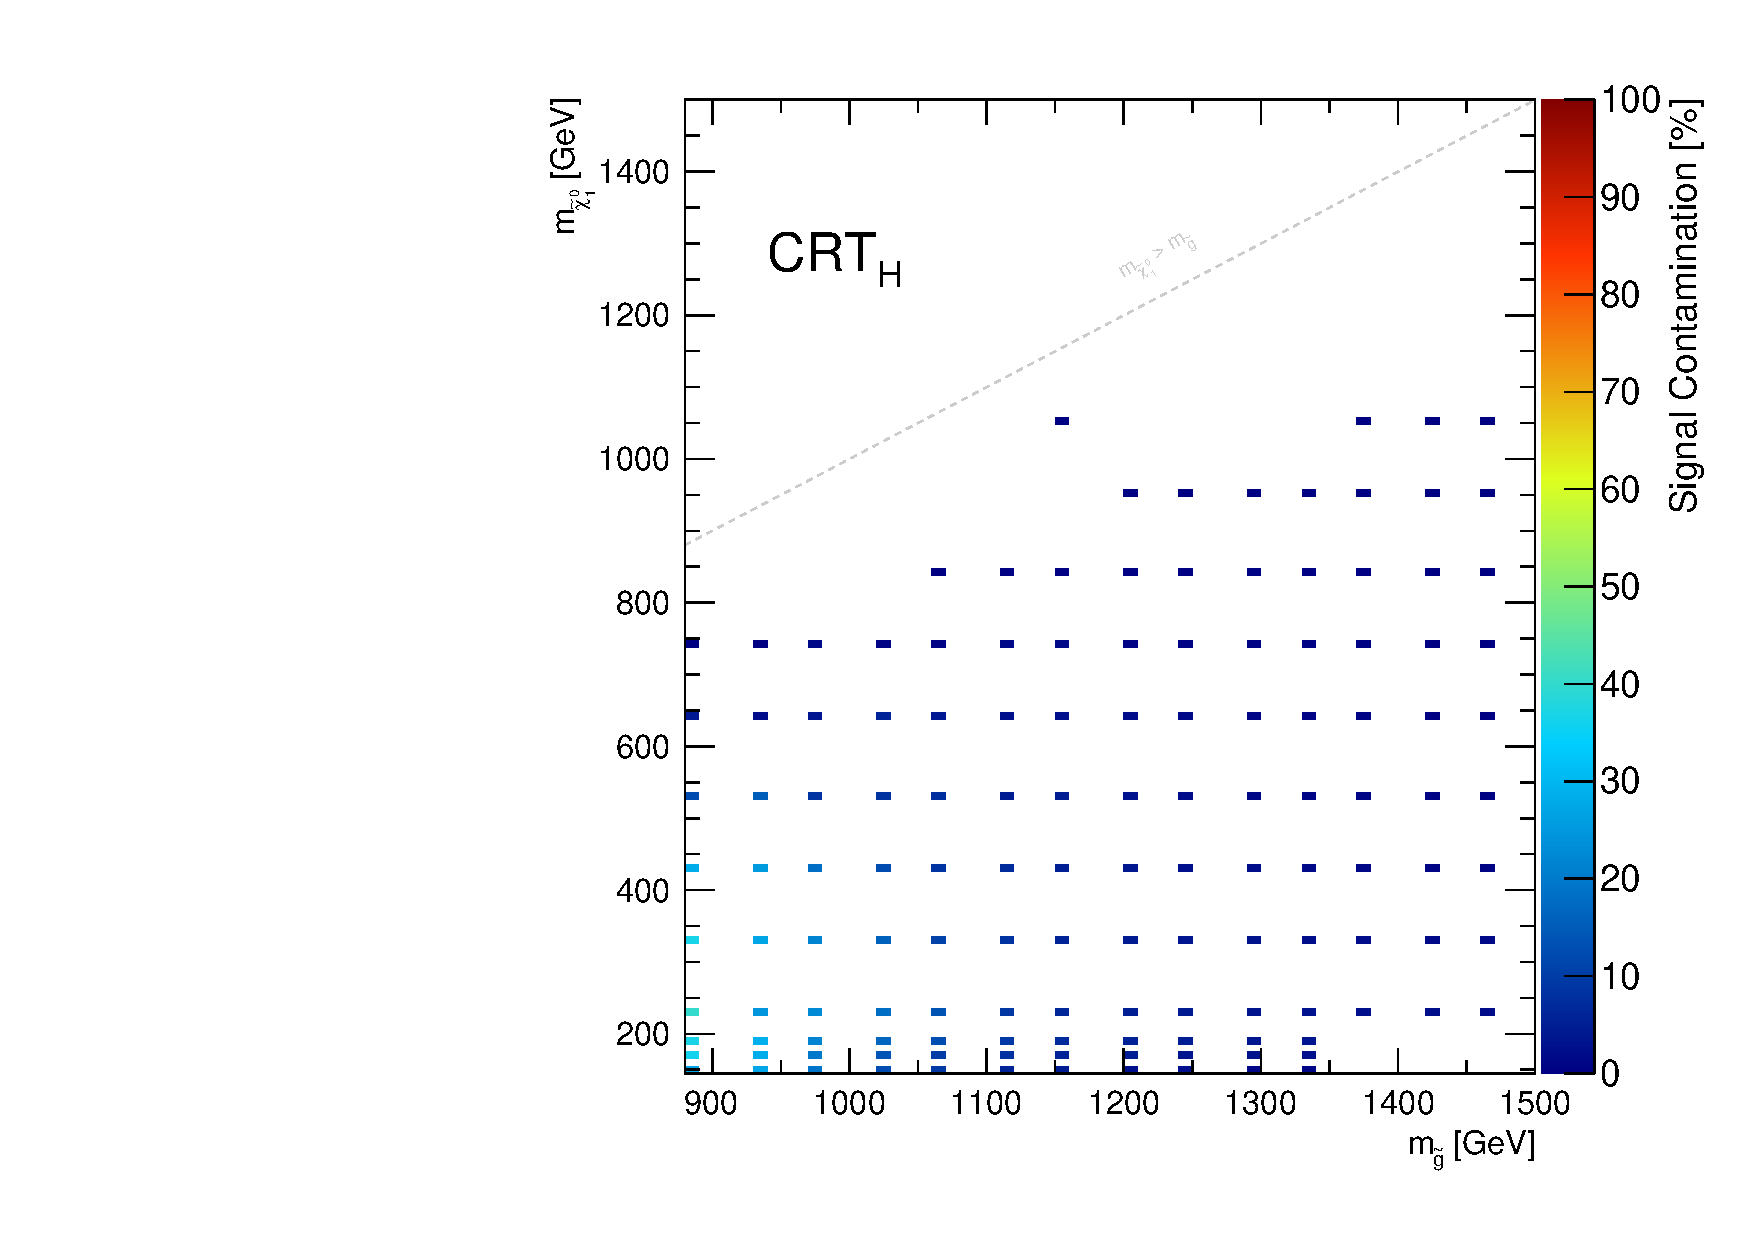
\includegraphics[width=0.46\textwidth]{signal_contamination_crth}

  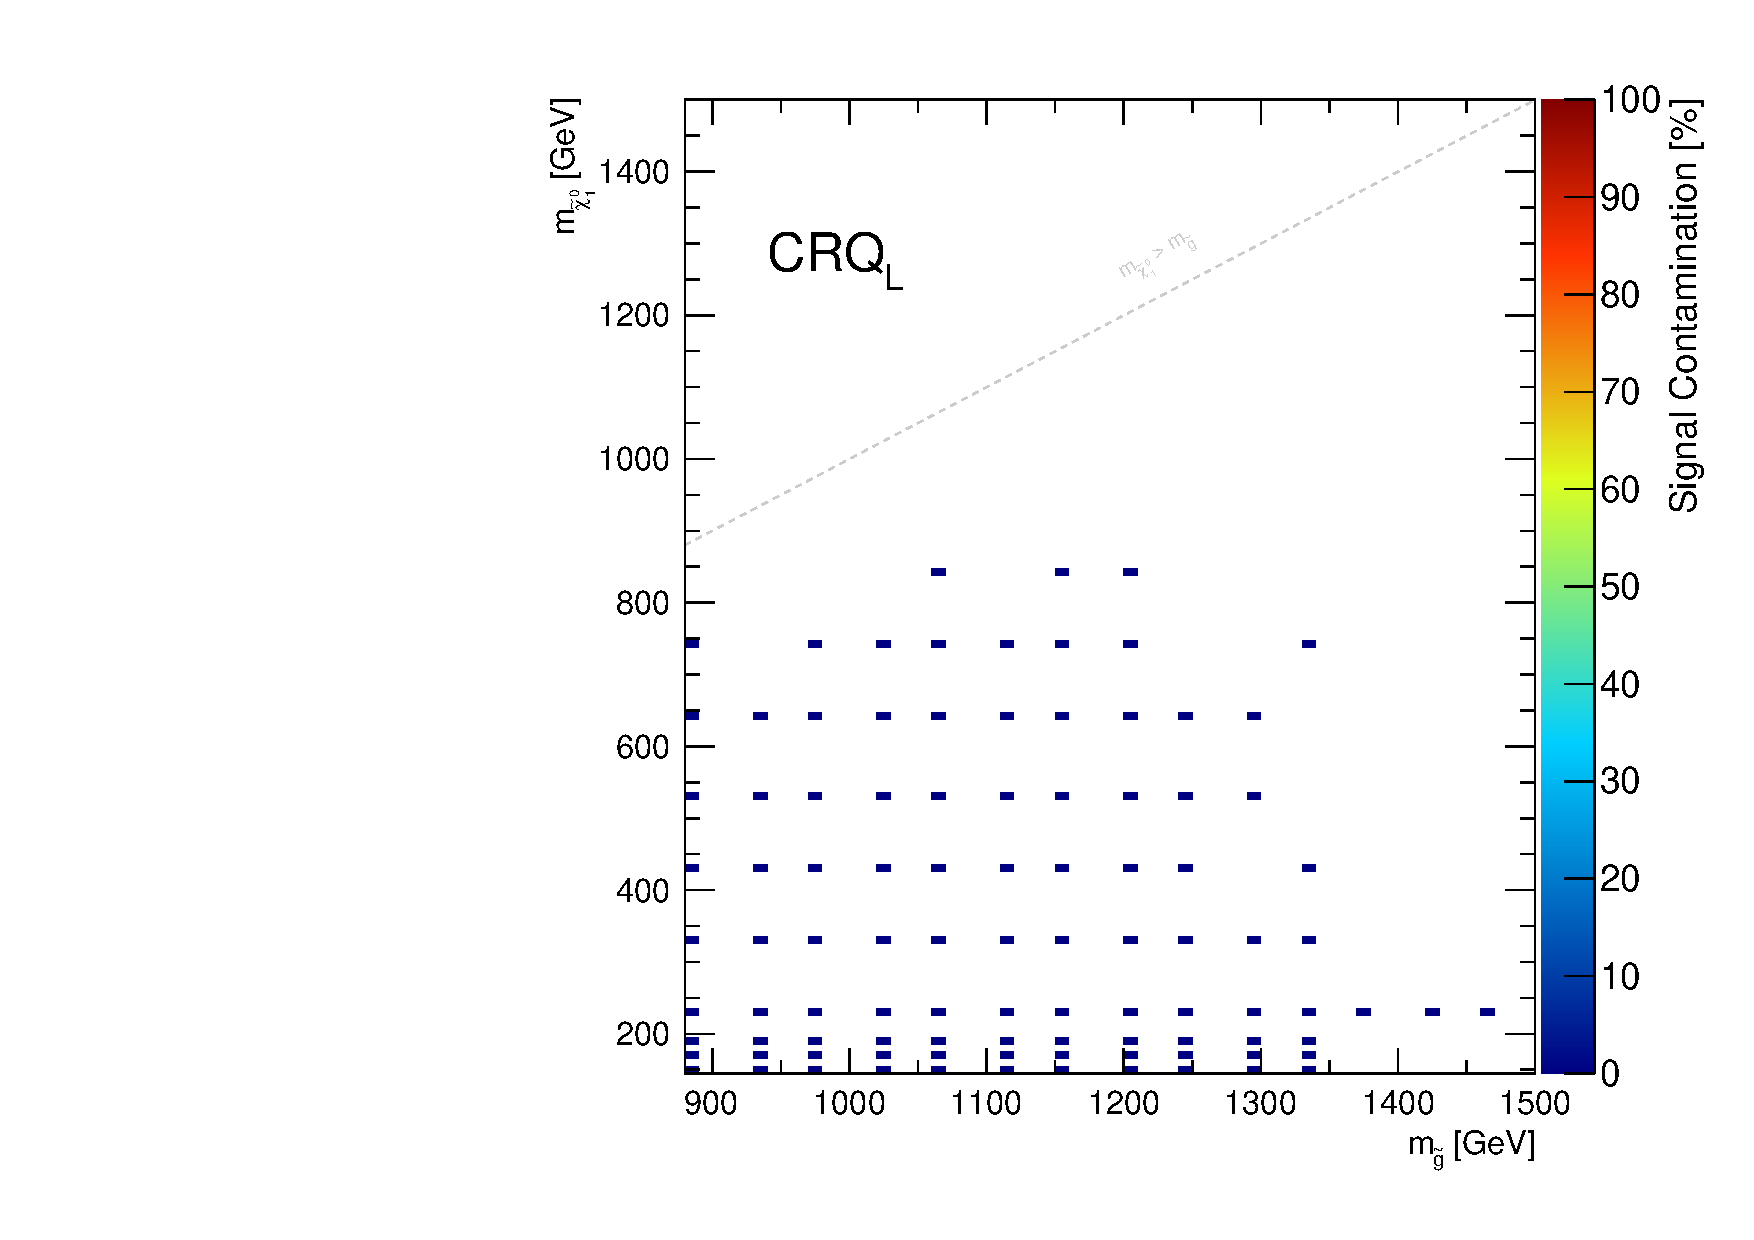
\includegraphics[width=0.46\textwidth]{signal_contamination_crql}\hspace{1cm}
  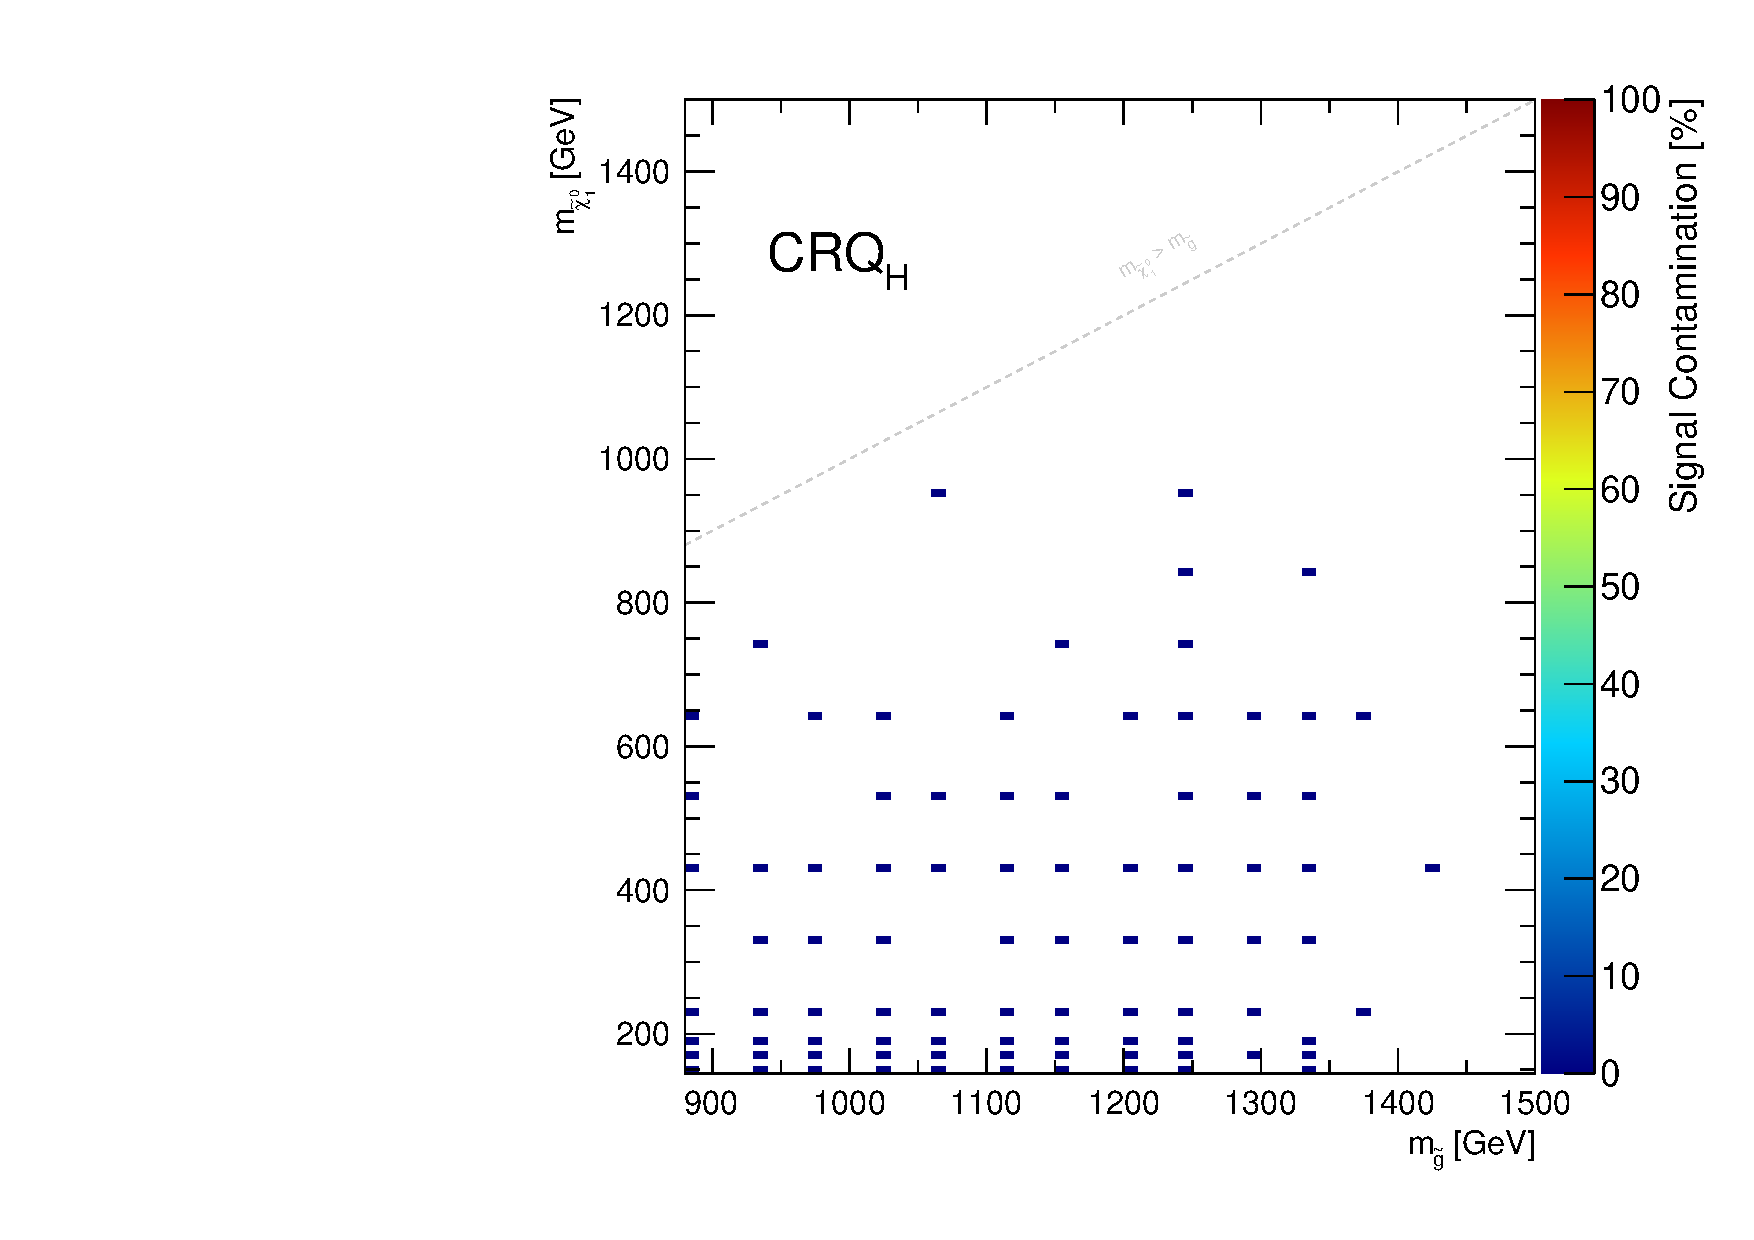
\includegraphics[width=0.46\textwidth]{signal_contamination_crqh}


  \caption{Contaminación de señal esperada en las regiones de control {\CRW} (arriba),
    {\CRT} (medio) {\CRQ} (abajo) asociadas a {\SRL} (izquierda) y {\SRH} (derecha).}
  \label{fig:bkg_cr_contamination}
\end{figure}



\subsection{Regiones de validación}

Como se mencionó anteriormente, en la definición de las regiones de control,
algunos cortes fueron relajados, o directamente removidos respecto a las SR,
para incrementar el número de eventos en las mismas. Para validar la
extrapolación entre las CR y la SR, se definen ciertas regiones de validación,
imponiendo nuevamente los cortes de la SR, de a uno a la vez.

De esta forma se definen las siguientes regiones de validación para {\CRW} y
{\CRT}, donde la X se refiere a la correspondiente CR (W o T). La selección
detallada puede verse en \cref{tab:bkg_vrs1}.

\begin{description}
\item[\textbf{VRXM}]  igual que CRX pero con el corte en {\met} como en la SR.
\item[\textbf{VRXR}]  igual que CRX pero con el corte en {\rt} como en la {\SRL} (solo para {\SRL}).
\item[\textbf{VRXH}]  igual que CRX pero con el corte en {\HT} como en la {\SRH} (solo para {\SRH}).
\end{description}

\begin{table}[!htbp]
  \centering

  \caption{Selección para las regiones de validación utilizadas para validar la extrapolación
    de los fondos de {\wgam}, {\ttgam}, entre las CR a las regiones de señal
    {\SRL} y {\SRH}}
  \label{tab:bkg_vrs1}

  \resizebox{\textwidth}{!}{
  \begin{tabular}{r|cccc|cccc}
    \hline
                                       & \multicolumn{4}{c|}{\SRL} & \multicolumn{4}{c}{\SRH} \\
    \cline{2-9}
                             &       VRWM &       VRWR &     VRTM &      VRTR &     VRWM &       VRWH &     VRTM &      VRTH \\
  \hline
  $\pt^\gamma$ [\gev] $>$    &        125 &        125 &      125 &      125  &      150 &        150 &      150 &      150  \\
  $N_\mathrm{leptones}$      &          1 &          1 &  $\ge 1$ &  $\ge 1$  &        1 &          1 &  $\ge 1$ &  $\ge 1$  \\
  {\met} [\gev]              &     $>200$ &  [100-200] &   $>200$ &  [80-200] &   $>300$ &  [100-200] &   $>300$ &  [80-200] \\
  $N_\mathrm{jets} \ge$      &          4 &          4 &        4 &         4 &        2 &          2 &        2 &         2 \\
  $N_{b\text{-jets}}$        &          0 &          0 &  $\ge 1$ &   $\ge 1$ &        0 &          0 &  $\ge 1$ &   $\ge 1$ \\
  $\pt^{j_1},\pt^{j_2}$ [\gev] $>$     &        100 &        100 &      100 &       100 &       40 &         40 &       40 &        40 \\
  $\dphijm >$                &        0.4 &        0.4 &      0.4 &       0.4 &      0.4 &        0.4 &      0.4 &       0.4 \\
  $\rt <$                    &          - &       0.85 &        - &      0.85 &        - &          - &        - &         - \\
  {\HT} [\gev] $>$           &          - &          - &        - &         - &        - &        800 &        - &       800 \\
  \hline
  \end{tabular}
  }

\end{table}



\section{Producción de fotones directos (\gjet)}
\label{sec:bkg_gjet}

Por diseño, la probabilidad de que eventos de procesos de producción de fotones
directos ({\gjet}) pasen a la región de señal es
baja, ya que resulta raro que estos eventos tengan una gran cantidad de {\met}.
Sin embargo, esta energía faltante puede ser producida por la mala
reconstrucción de la energía de los jets, y debido a que la sección eficaz de
estos procesos es muy alta, puede resulta en una contaminación significativa.

Para determinar este fondo no es posible confiar plenamente en las simulaciones
MC, debido a que la baja cantidad de eventos similares a la señal implicaría
usar una muestra con una muy alto número de eventos que resulta dificultoso desde un
punto de vista computacional. Por este motivo se diseñó
una región de control dominada por eventos de {\gjet} a la que se llamó {\CRQ}.
Los detalles de la selección se pueden ver en la \cref{tab:bkg_crs}. Básicamente
es la misma selección que la SR pero requiriendo baja energía faltante ($\met <
50 \gev$).

%% La estimación final del fondo de fotones directos es obtenida entonces normalizando los
%% eventos de la muestra MC en esta region de control.
%% The final estimate for the prompt photon background is obtained by normalizing the Sherpa MC events passing a dedicated selection (CRM) defined
%% from the corresponding SR but at low {\met} ($< 50 \gev$). As expected,  CRM selects an enriched sample %of events with similar kinematics to the SR but enriched in
%% of QCD background events. The multijet contamination is independently estimated with the ratio method explained in sec \ref{sec:jetfakes}. %, is explicitly removed from the selected sample to avoid double counting in the global fit described in sec \ref{sec:fitconfig}
%% Some intermediate {\met} regions between 50 {\gev} and the SR cut are kept for validation purposes. Given the large jet multiplicty and \MET requirements in SR2 and SR3, respectively, the prompt photon background is
%% expected to be very small in both signal regions. However, its contribution is not negligible in the control and validation regions so it is important to get a good normalization estimate.

%% ## CRM_2
%% Percentage of photonjet_sherpa:  87.65 % 1224.78869629 / 1397.31749731
%% Largest contamination:  0.67 %

%% ## CRM_3
%% Percentage of photonjet_sherpa:  87.54 % 156.909103394 / 179.23669574
%% Largest contamination:  0.35 %

La contaminación de señal en esta región de control es despreciable, debido a
que la señal posee gran cantidad de energía faltante, como puede verse en la
\cref{fig:bkg_cr_contamination}.

%% \begin{figure}[!htbp]
%%   \centering
%%   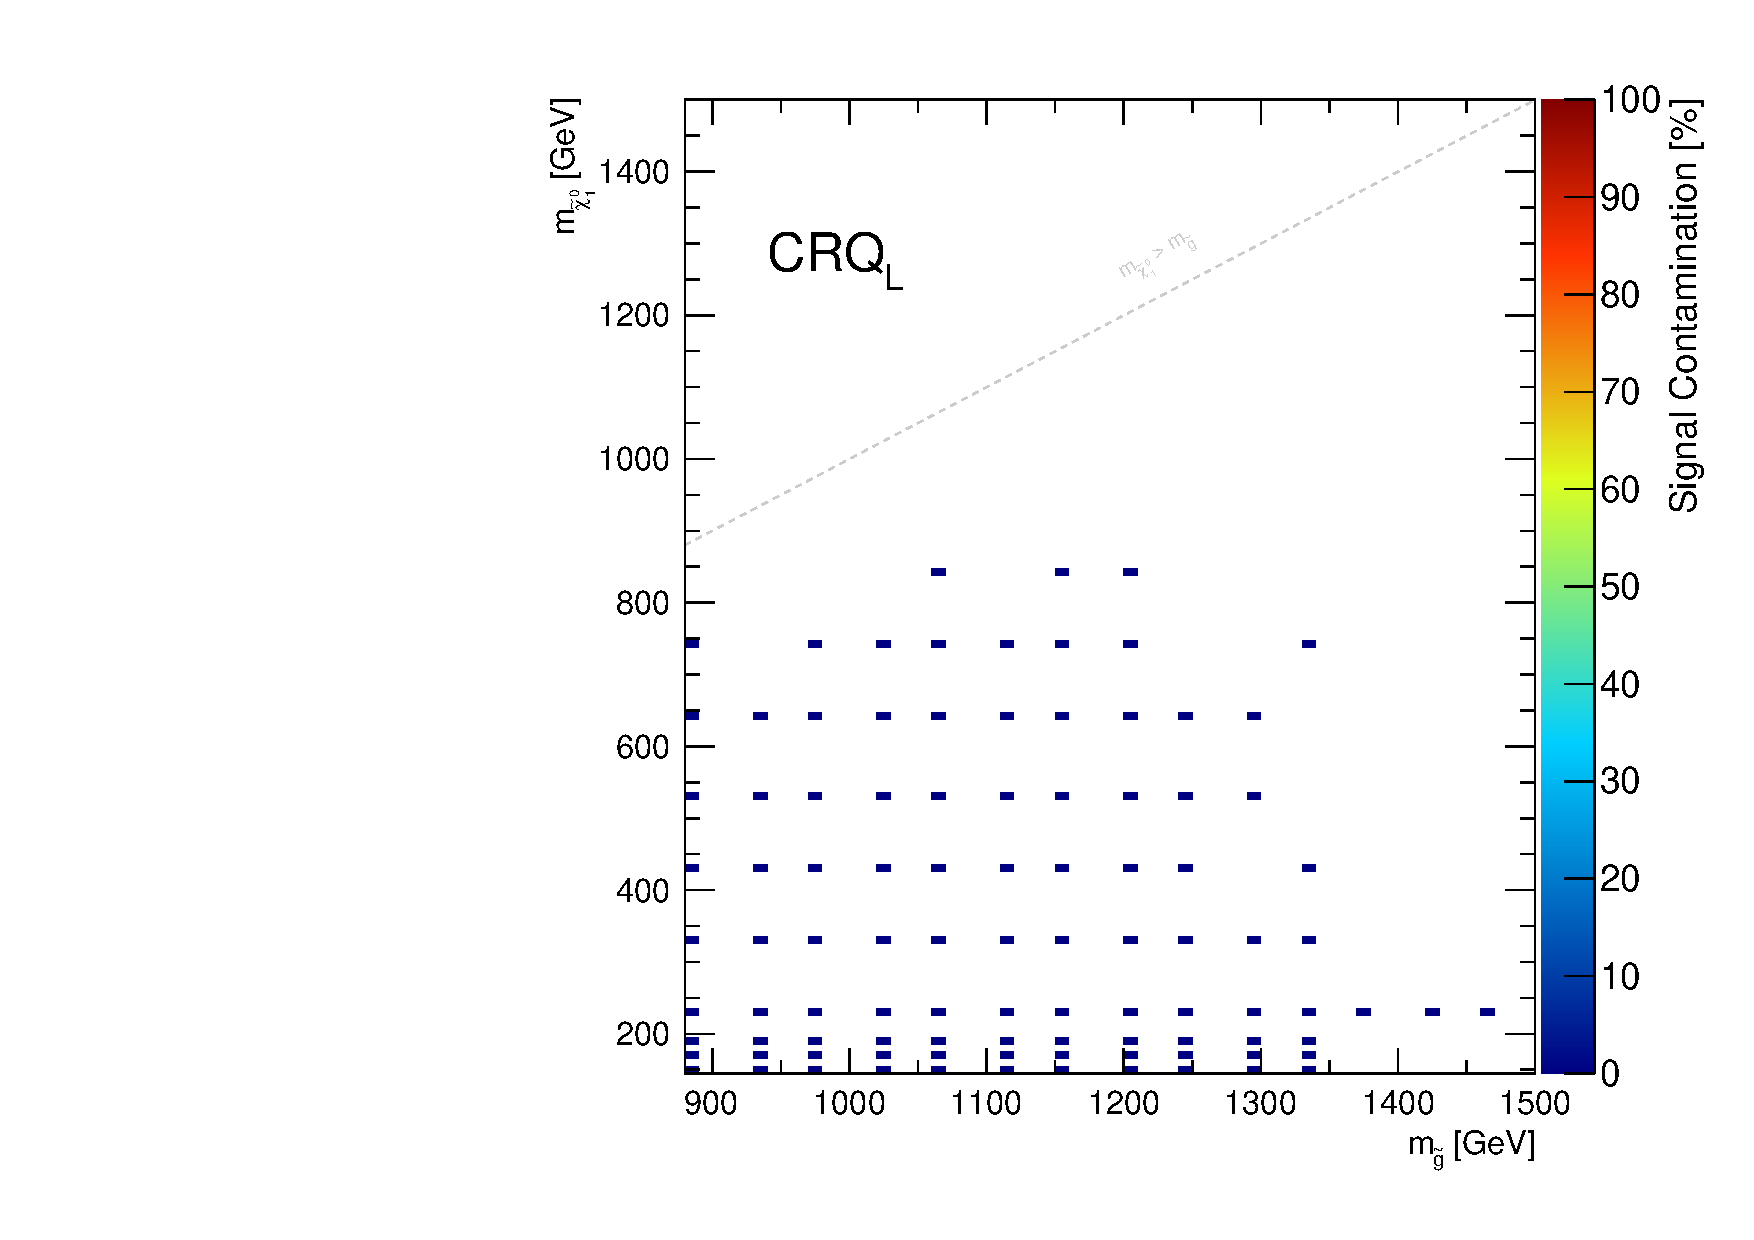
\includegraphics[width=0.49\textwidth]{signal_contamination_crql}
%%   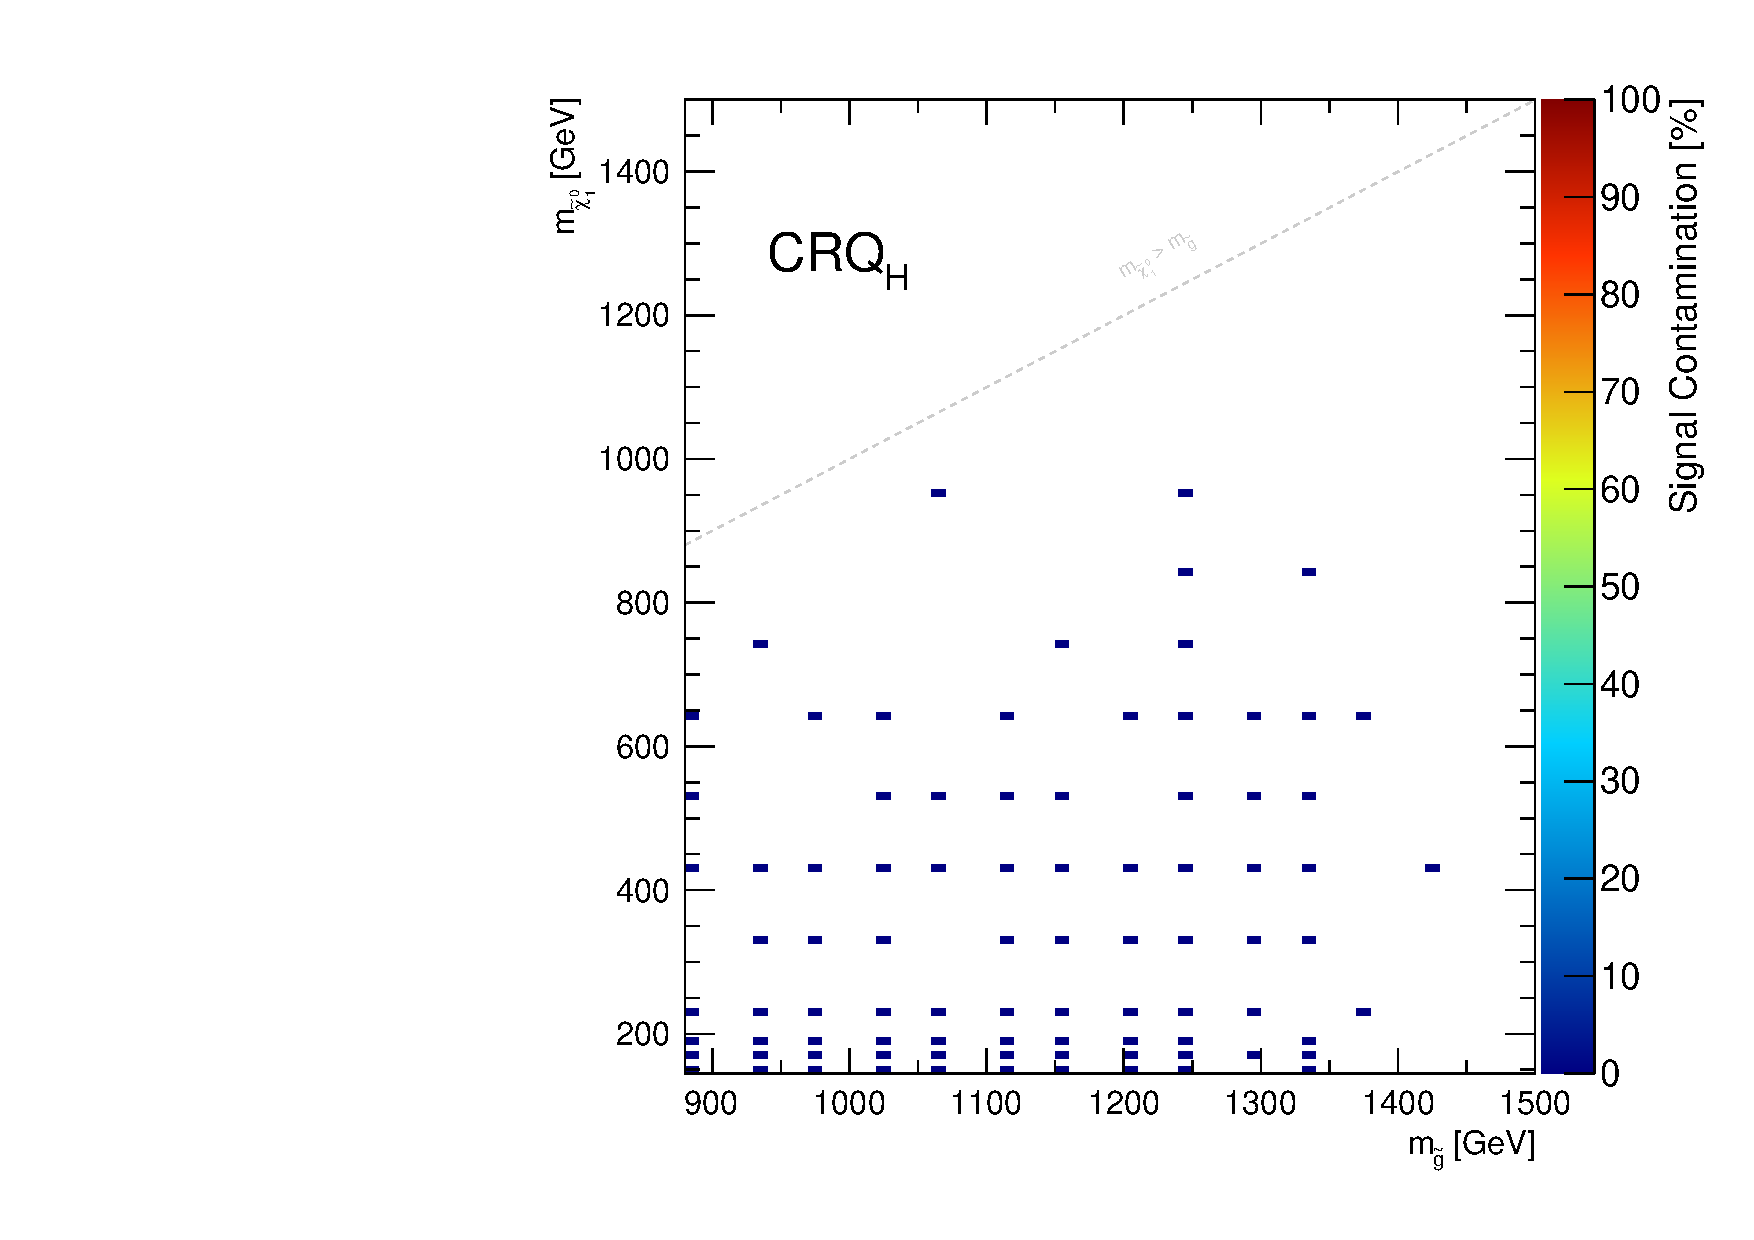
\includegraphics[width=0.49\textwidth]{signal_contamination_crqh}

%%   \caption{Contaminación de señal esperada en la región de control {\CRQ} asociada a {\SRL} (izquierda) y {\SRH} (derecha).}
%%   \label{fig:bkg_cr_contamination}
%% \end{figure}


%% \subsection{Comparación de generadores}

%% Acá comparación entre Pythia y Sherpa


\subsection{Regiones de validación}\label{sec:bkg_vrs2}

Con un conjunto de cortes de selección se definen regiones para validar los resultados de la
extrapolación de {\gjet} de la región de control a bajo {\met} hasta
las SR a alto {\met}. Las regiones de validación deben estar lo más cerca posible
de las SR en el espacio de observables, pero deben ser ortogonales a las mismas.
Esto se logra invirtiendo algunos cortes, como se describe a continuación.

\begin{description}\itemsep0.1cm
\item[{\bf VRMX}] igual a la SR pero con un requerimiento intermedio en {\met}
  ($X\gev < \met < 150\gev$) con $X = 75,100$. El corte superior asegura la
  ortogonalidad con la SR.
\item[{\bf VRH}] igual a la SR pero invirtiendo el corte en {\HT} ($\HT<
  800\gev$). Solo definida para {\SRH}, ya que no hay un corte en {\HT} en
  {\SRL}.
\item[{\bf VRQ}] igual a la SR pero invirtiendo el corte en {\dphijm} ($\dphijm < 0.4$)
  para aumentar la contribución de fondos con {\met}
  instrumental.
\end{description}

En la \cref{fig:bkg_crq} pueden verse los esquemas de la definición de las CR y VR.

\begin{figure}[!htbp]
  \centering

  \resizebox{0.49\textwidth}{!}{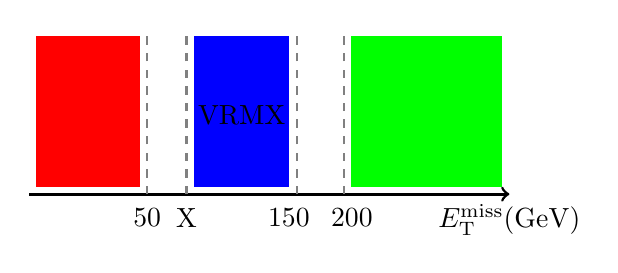
\begin{tikzpicture}[domain=0:4]

  \tikzstyle{region} = [fill]

  \draw[line width=1, ->] (0,0) -- (6.1,0) node[below] {$E_\mathrm{T}^\mathrm{miss} (\mathrm{GeV})$};
  %% \draw[line width=1, ->] (0,0) -- (0,3.1);

  \draw[gray, dashed, line width=0.8] (1.5, 0) -- (1.5, 2.1);
  \draw[gray, dashed, line width=0.8] (4.0, 0) -- (4.0, 2.1);
  \draw[gray, dashed, line width=0.8] (2.0, 0) -- (2.0, 2.1);
  \draw[gray, dashed, line width=0.8] (3.4, 0) -- (3.4, 2.1);

  \draw node at (1.5,-0.3) {50};
  \draw node at (2.0,-0.3) {X};
  \draw node at (3.3,-0.3) {150};
  \draw node at (4.1,-0.3) {200};

  \draw[green, region] (4.1,0.1) rectangle (6,2);
  \draw node at (5.0,1) {\SRL};

  \draw[red, region] (0.1,0.1) rectangle (1.4,2) ;
  \draw node at (0.75, 1) {\CRQ};

  \draw[blue, region] (2.1,0.1) rectangle (3.3,2) ;
  \draw node at (2.7,1) {VRMX};


\end{tikzpicture}
}
  \resizebox{0.49\textwidth}{!}{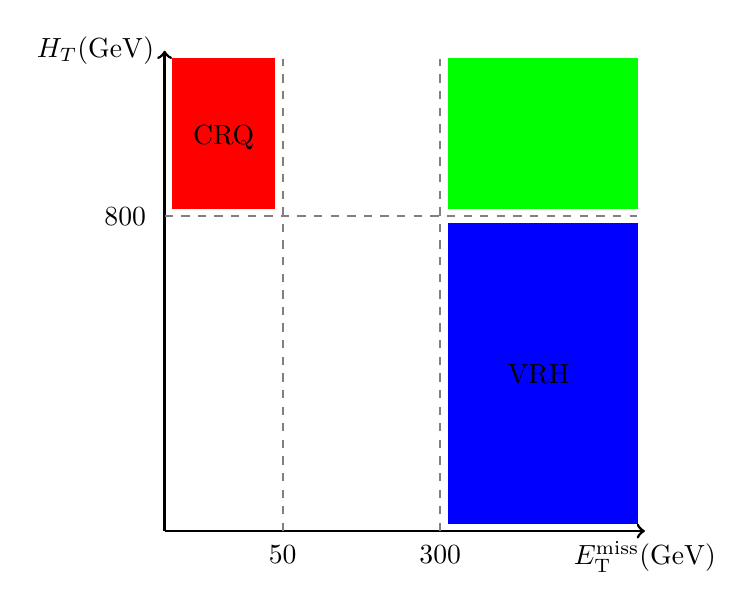
\begin{tikzpicture}[domain=0:4]

  \tikzstyle{region} = [fill]


  \draw[line width=1, ->] (0,0) -- (0,6.1) node[left] {$H_T (\mathrm{GeV})$};
  \draw[line width=1, ->] (0,0) -- (6.1,0) node[below] {$E_\mathrm{T}^\mathrm{miss} (\mathrm{GeV})$};

  %% \draw[gray, dashed, line width=0.8] (0, 2.5) -- (6, 2.5);
  \draw[gray, dashed, line width=0.8] (0, 4.0) -- (6, 4.0) node[black] at (-0.5,4.0) {800};
  \draw[gray, dashed, line width=0.8] (1.5, 0) -- (1.5, 6) node[black] at (1.5,-0.3) {50};
  \draw[gray, dashed, line width=0.8] (3.5, 0) -- (3.5, 6) node[black] at (3.5,-0.3) {300};

  \draw[green, region] (3.6,4.1) rectangle (6,6);
  \draw node at (4.75,5.0) {\large \SRH};

  \draw[red, region] (0.1,4.1) rectangle (1.4,6) ;
  \draw node at (0.75, 5) {CRQ};

  \draw[blue, region] (3.6,0.1) rectangle (6,3.9) ;
  \draw node at (4.75,2.) {VRH};

\end{tikzpicture}
}

  \caption{Esquema de las regiones de control diseñadas para normalizar el fondo
    de {\gjet} para {\SRL} (izquierda) y {\SRH} (derecha). También se muestran
    las regiones de validación utilizadas para validar la extrapolación
    $\mathrm{CR}\to\mathrm{SR}$.}
  \label{fig:bkg_crq}
\end{figure}



%----------------
% Electron fakes
%----------------
\section{Electrones identificados como fotones} \label{sec:efakes}

Los eventos en los que un electrón de alto {\pt} es identificado como un
fotón \cite{Bocci:1643300} pueden contaminar alguna de las SR. Esta contaminación
proviene generalmente de procesos del SM como $W(\to e\nu)$+ jets, $Z(\to ee)$ +
jets y {\ttbar}.

Como se mencionó en la \cref{sec:obj_photons}, los electrones y fotones dejan
lluvias electromagnéticas muy similares en el detector. Los algoritmos de
reconstrucción de fotones están diseñados para reducir la identificación errónea
de electrones como fotones aunque, para poder mantener una alta eficiencia de
reconstrucción, no se realiza una distinción demasiado estricta. En caso de
duda, los clusters electromagnéticos son reconstruidos bajo ambas hipótesis
(electrón o fotón) y guardados (duplicados) en ambas categorías. Esto implica
que algunos electrones pueden terminar siendo reconstruidos como fotones, y si
estos pasan la selección de fotones utilizada en el análisis, contribuirán al
fondo por mala identificación $e\to\gamma$.

Los electrones son reconstruidos a partir de los clusters asociados a una traza,
mientras que los fotones son reconstruidos de los clusters que no tienen ninguna
traza asociada (candidatos a fotones no-convertidos) o están asociados a un
vértice de conversión (candidatos a fotones convertidos). Se consideran los
vértices con una o dos trazas en la reconstrucción de fotones convertidos, y por
lo tanto los fotones convertidos pueden ser categorizados como fotones
convertidos con una traza o dos trazas. La traza de los candidatos a fotón
convertidos con una sola traza debe poseer un impacto en la \emph{B-layer}. Se
espera que una fracción de electrones pueda ser reconstruida como fotones
convertidos, por ejemplo, si falla la asociación de la traza a un impacto en la
B-layer, o si se asocia un vértice de conversión espurio a ella. Asimismo, el
electrón puede ser reconstruido como un fotón no-convertido si falla el
algoritmo que asocia la traza al cluster .

La fracción de electrones reconstruidos como fotones, depende claramente del
material en el detector, es por eso que pueden existir diferencias si se calcula
a partir de simulaciones Monte Carlo, ya que el material en las simulaciones no
es perfecto. Por tal motivo se calcula a partir de los datos, aunque también se
realiza una comparación con las muestras MC.
El número de eventos de electrones reconstruidos como fotones en la región de
señal ($N_{e\to\gam}^{\mathrm{SR}}$) se obtiene multiplicando esta fracción (\feg)
por el número de eventos en la muestra de electrones
obtenida invirtiendo el rol de fotones y electrones en la selección de la región
de señal ($N_e^{\mathrm{SR}}$). Para calcular este número de eventos se requiere
un electrón aislado de alto {\pt}, y los fotones de señal son
vetados.

\begin{equation}
  N_{e\to\gam}^{\mathrm{SR}} = \feg \cdot N_e^{\mathrm{SR}}
\end{equation}

Para estimar {\feg} se utiliza un método llamado \emph{tag and probe}, en una muestra
de eventos de datos {\Zee} que pasan el mismo trigger de fotones que utiliza el
análisis y la misma preselección. Adicionalmente, se
aplica un corte de $\met < 40 \gev$ para reducir la posible contaminación de
fotones reales de eventos de {\wgam}.

El método consiste en seleccionar un electrón (el electrón \emph{tag}) que
pasa un criterio de identificación \emph{tight} y que tiene $20 \gev < \pt < 125 \gev$.
Luego se busca un segundo candidato a electrón o fotón
(el objeto \emph{probe}). Este puede ser un electrón \emph{tight} o un fotón
\emph{tight}, ambos con $\pt > 125\gev$ y satisfaciendo los requerimientos de
aislamiento correspondientes.

Los valores de la masa de los pares de objetos seleccionados son guardados
separadamente para los tres casos posibles: dos electrones, un electrón y un
fotón convertido, o un electrón y fotón no-convertido. En los tres casos se
puede ver un pico alrededor del valor de la masa del bosón $Z$ ($\sim 91
\gev$).
Como el bosón $Z$ no puede decaer directamente en un electrón y un fotón, los
pares electrón-fotón que aparecen bajo el pico del $Z$ corresponden a electrones
mal identificados. Sin embargo, lo mismo aplica a otros procesos que contienen
dos electrones en estado final.
Por lo tanto es necesario utilizar algún método de
sustracción del fondo. Este deberá también tener en cuenta la contaminación por
las combinaciones aleatorias.

La probabilidad de identificación errónea {\feg} puede estimarse entonces como:

\begin{equation}\label{eq:efakerate}
  \feg = \frac{N_{e\gam}}{N_{ee}}
\end{equation}
%
donde $N_{e\gam}$ ($N_{ee}$) es el número de pares electrón-fotón
(electrón-electrón) encontrados en una ventana alrededor del pico del bosón $Z$ en la distribución de
la masa invariante, definida en el rango $81 < m_{ex} < 101 \gev$. Para obtener
el número de eventos $N_{ex}$, se realiza un ajuste de la distribución de la
masa invariante para los dos tipos de eventos utilizando un modelo de
señal+fondo. Este procedimiento se lleva a cabo de forma separada para fotones
convertidos y no-convertidos, y en clases del {\abseta} de los objetos
\emph{probe}. El bajo número de eventos disponibles hace imposible utilizar
clases de {\pt}, aunque de esta forma la estimación es conservativa ya que la
probabilidad de identificación errónea decrece con el {\pt} del electrón
\cite{Kuhl:1604846}.

Como modelo de señal se utiliza la suma de función \emph{Crystall-Ball} y una
Gausiana, mientras que para el modelo de fondo se utiliza un polinomio de grado
dos. En la \cref{fig:invmass_pairs} se pueden ver las distribuciones de la masa
invariante para pares de $ee$ y $e\gam$, para la selección inclusiva, y los
correspondientes ajustes del modelo.

\begin{figure}[!htb]
  \centering

  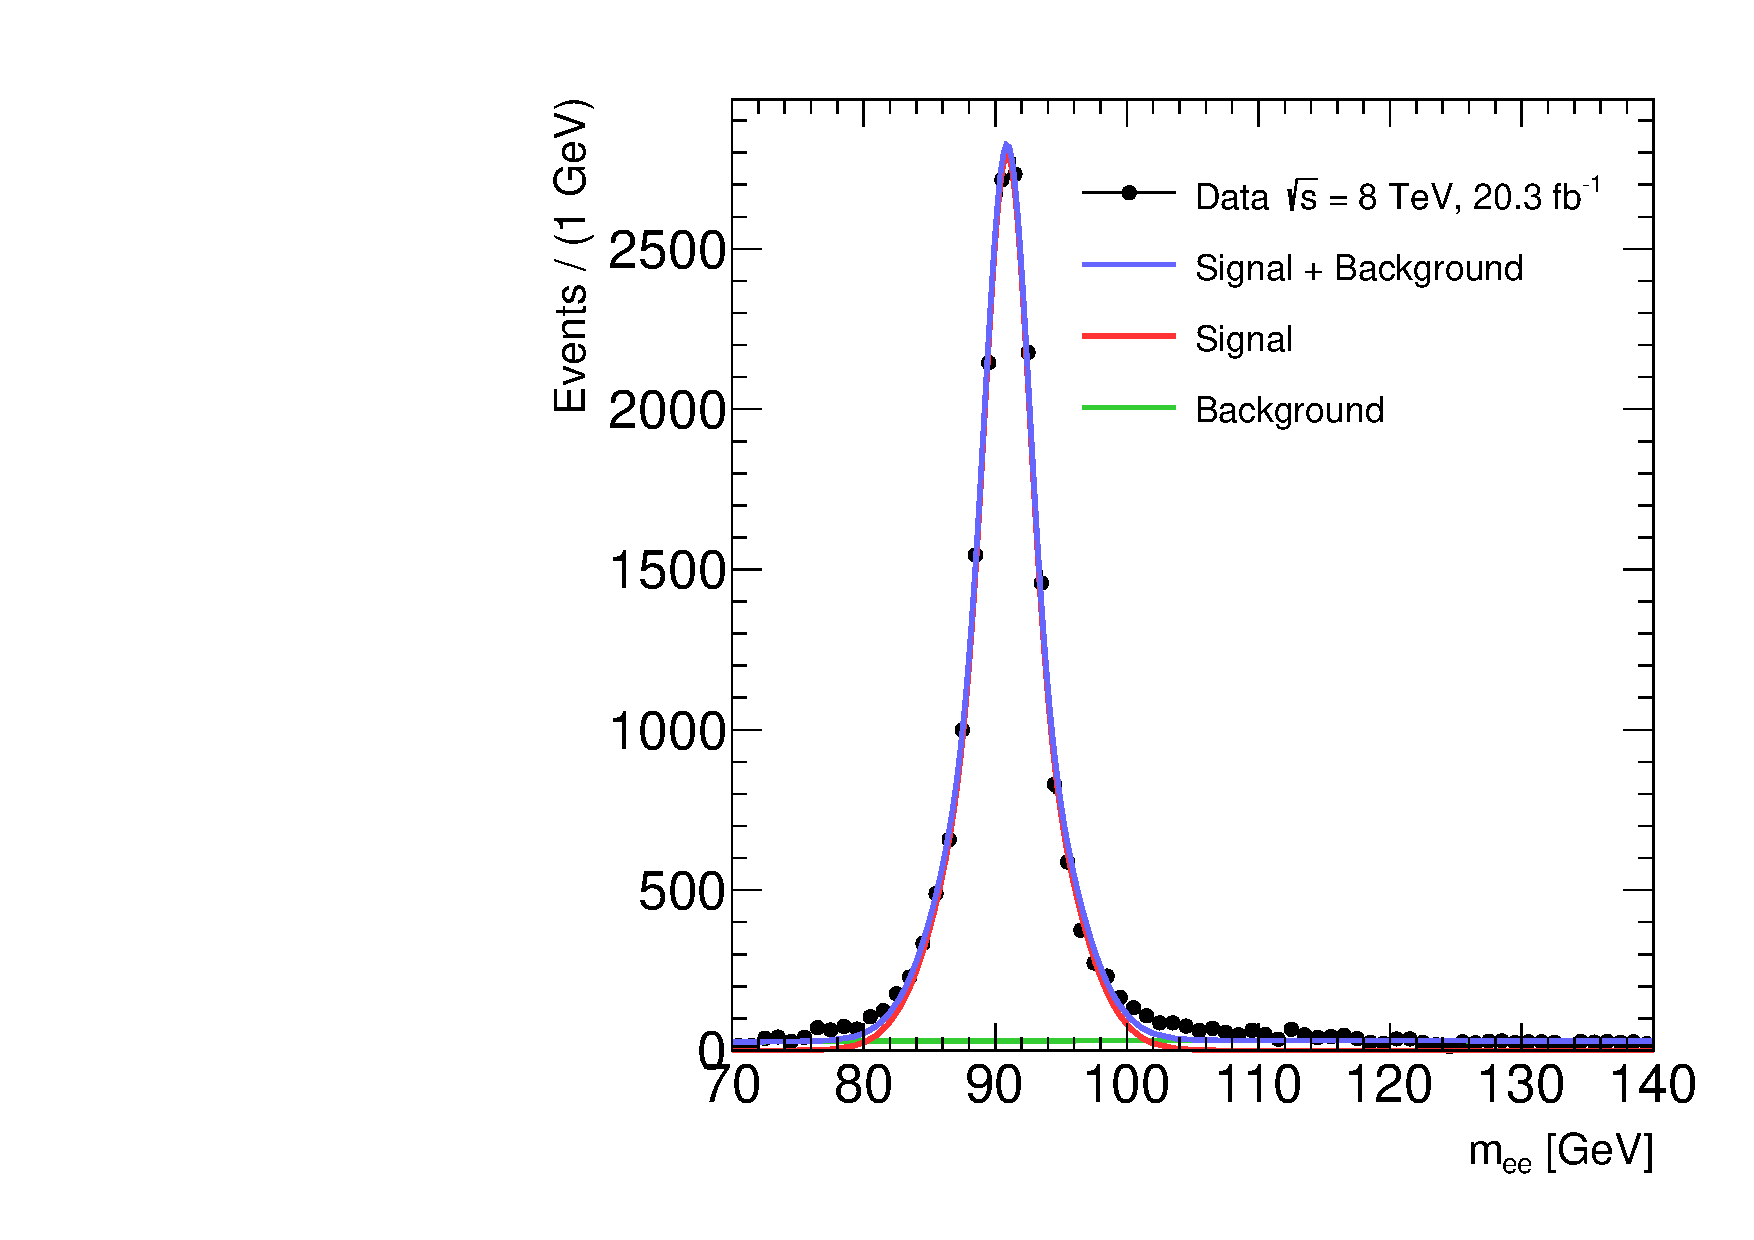
\includegraphics[width=0.49\textwidth]{figures/Fit_mee_efakes_Data_all}
  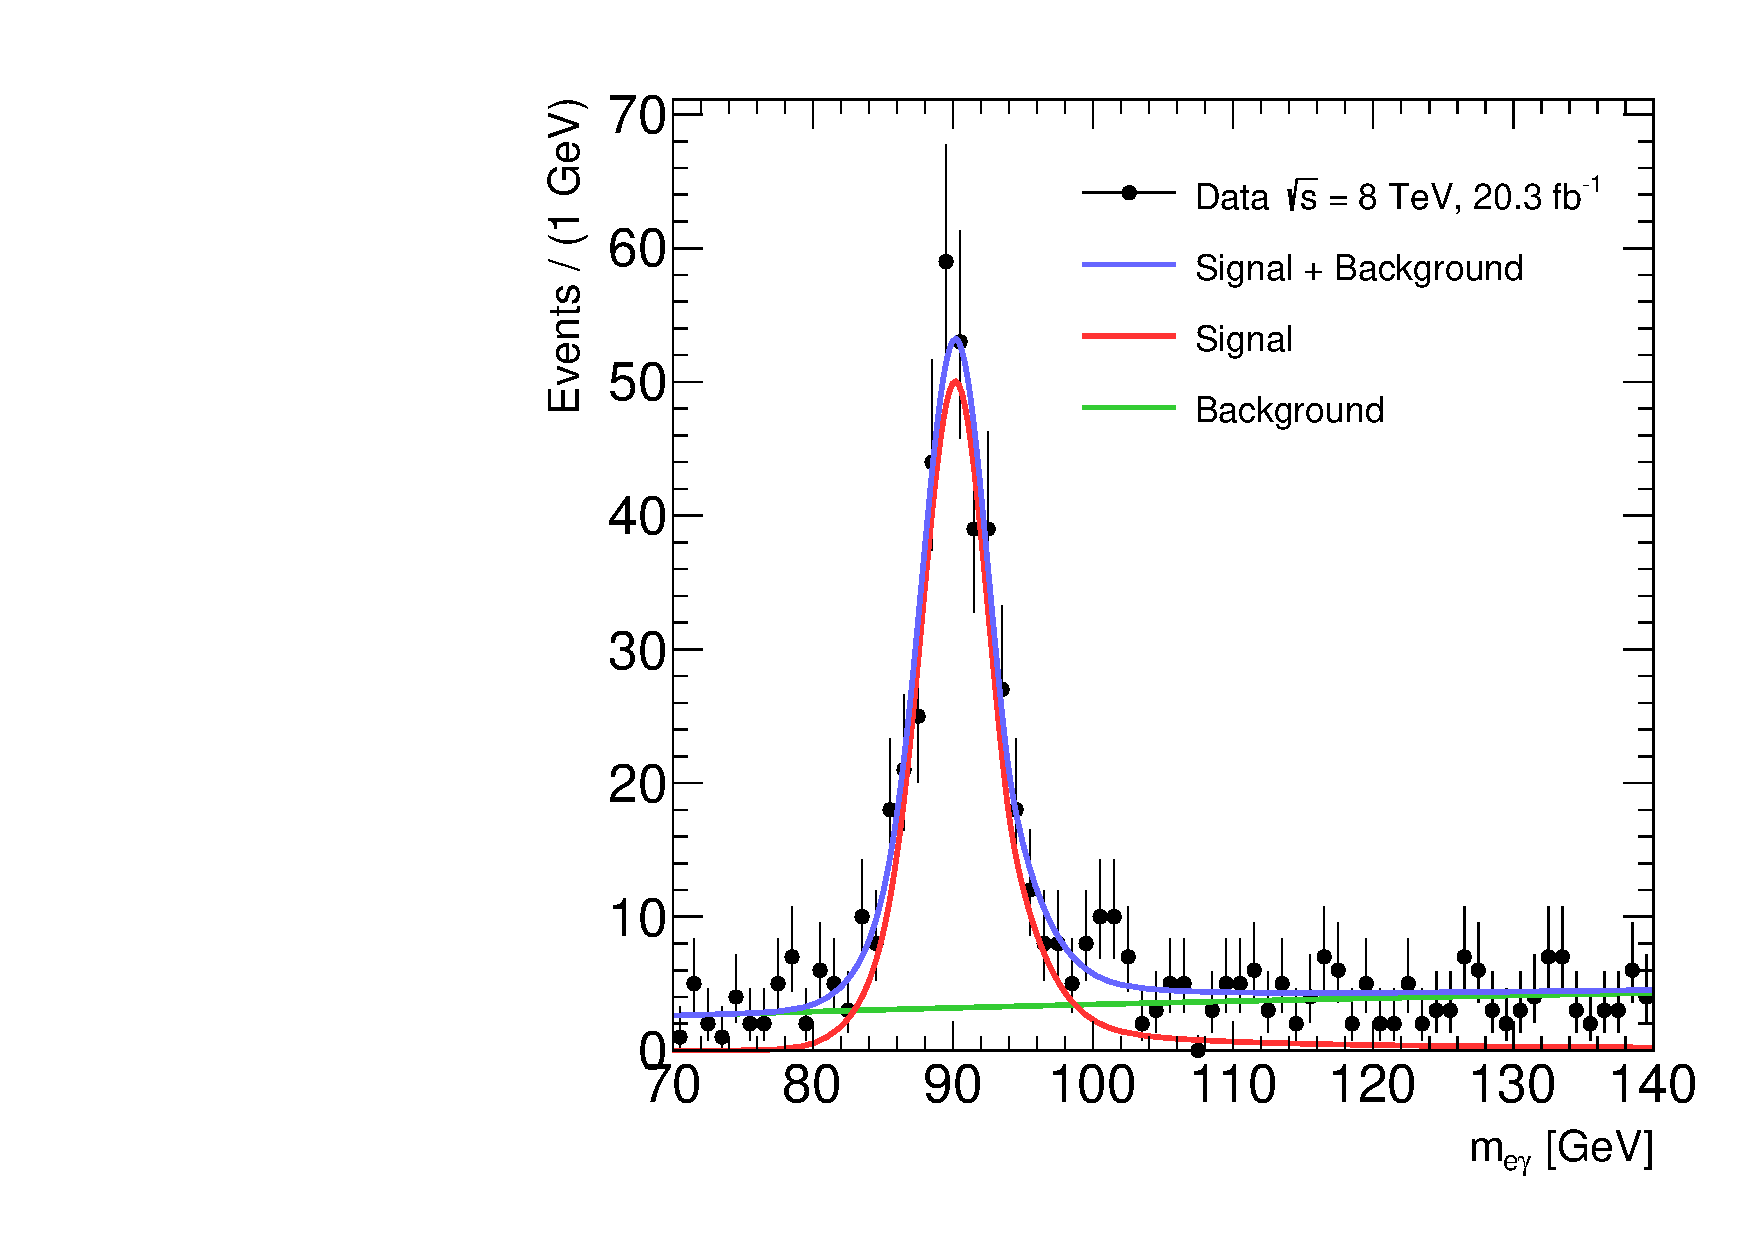
\includegraphics[width=0.49\textwidth]{figures/Fit_meg_efakes_Data_all}
  \caption{Distribuciones de la masa invariante de los pares de
    electrón-electrón (izquierda) y electrón-fotón (derecha). Se puede ver también el ajuste
    con el modelo de señal + fondo.}
  \label{fig:invmass_pairs}

\end{figure}

La probabilidad de identificación errónea se muestra en la \cref{fig:efake_eta},
como función del {\abseta} del objeto \emph{probe} para ``fotones'' convertidos
y no-convertidos. Este factor crece con {\abseta}, dado que está relacionado
con el incremento en el material del detector atravesado por los electrones y el
incremento en la tasa de reconstrucción de fotones convertidos con una sola
traza.

El {\feg} calculado a partir de los datos es comparado con el calculado a partir
de muestras MC de eventos de {\Zee} producidas con los generadores {\sherpa} y
{\powheg}. Se encuentra un buen acuerdo para todos los casos dentro de sus incertezas.
Los valores calculados de {\feg} pueden verse en la \cref{tab:efake_eta}, y \cref{tab:efake_uc} para fotones
convertidos y no-convertidos de forma separada.

\begin{figure}[!htb]
  \centering

  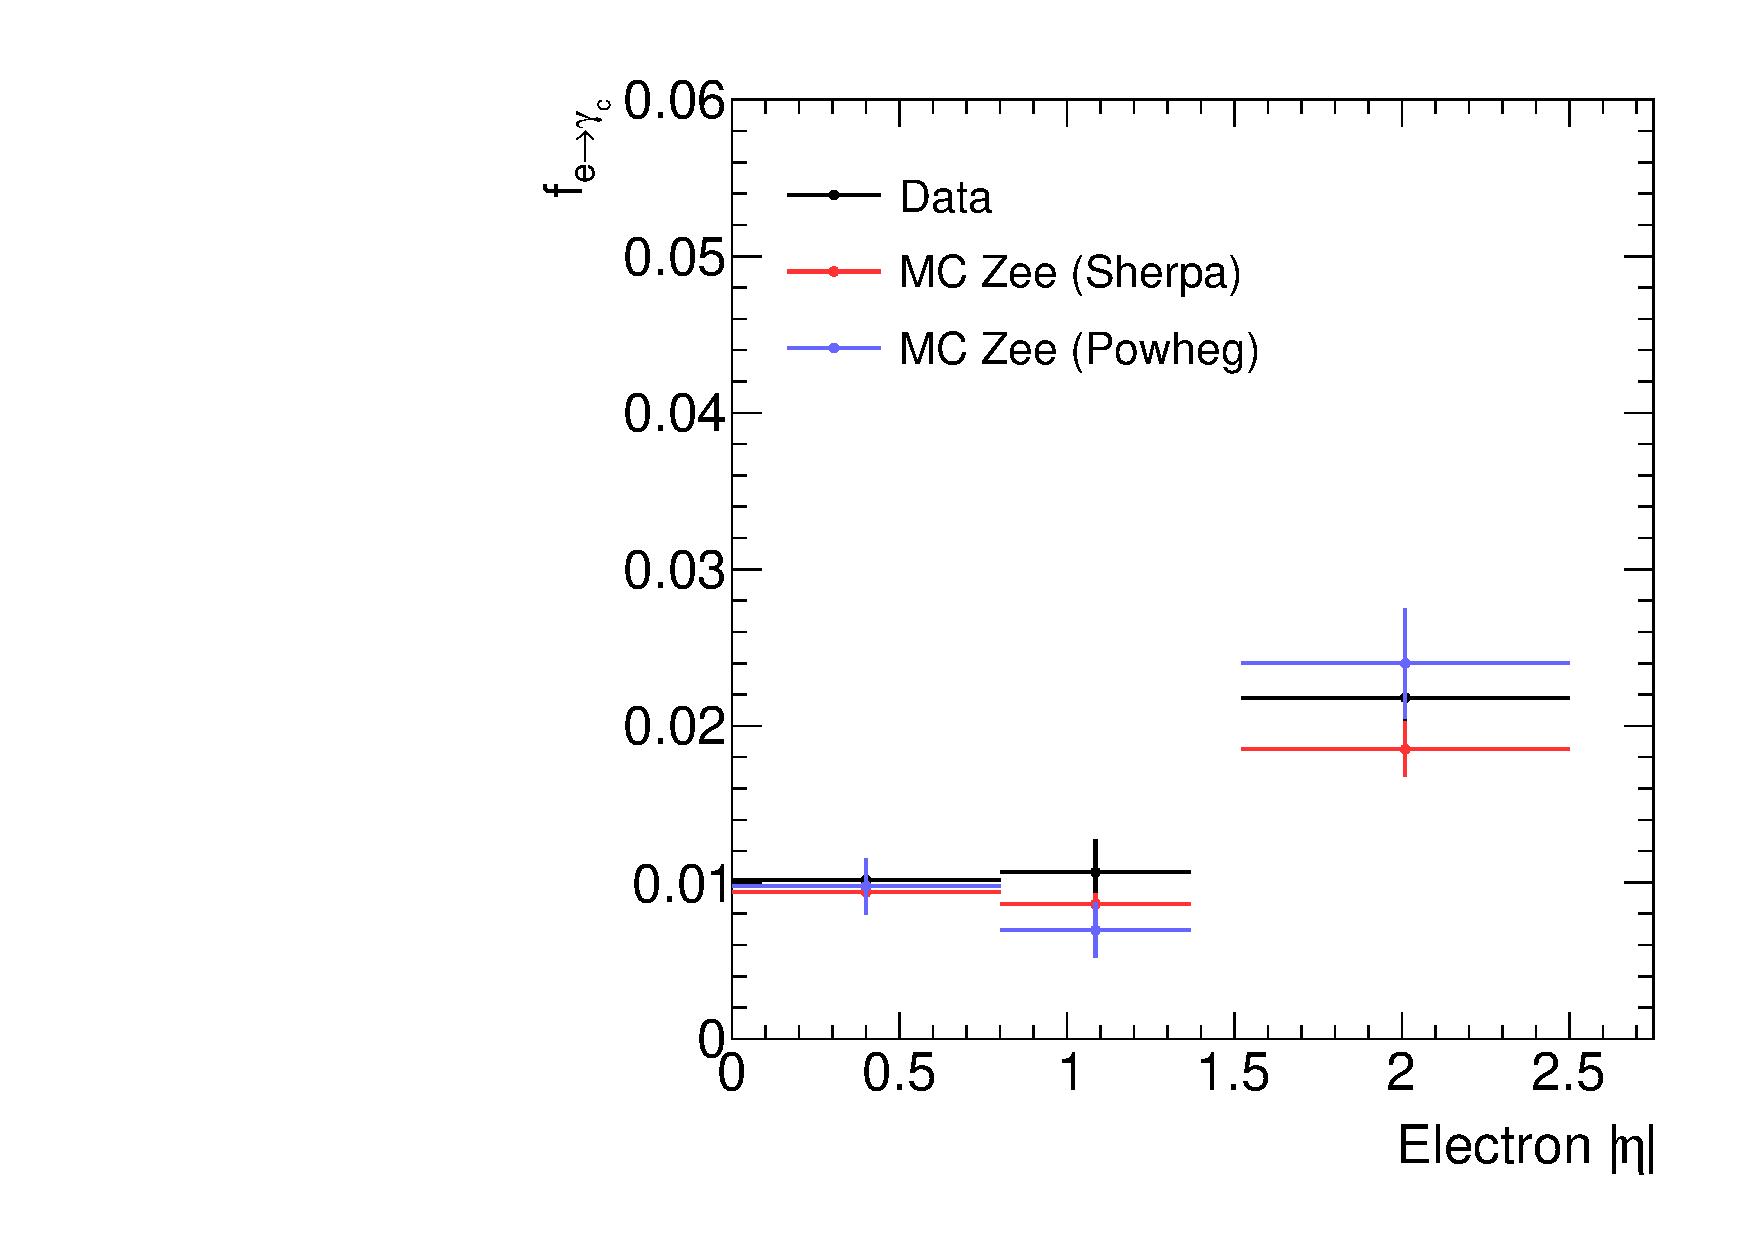
\includegraphics[width=0.45\textwidth]{figures/fegc_feta}
  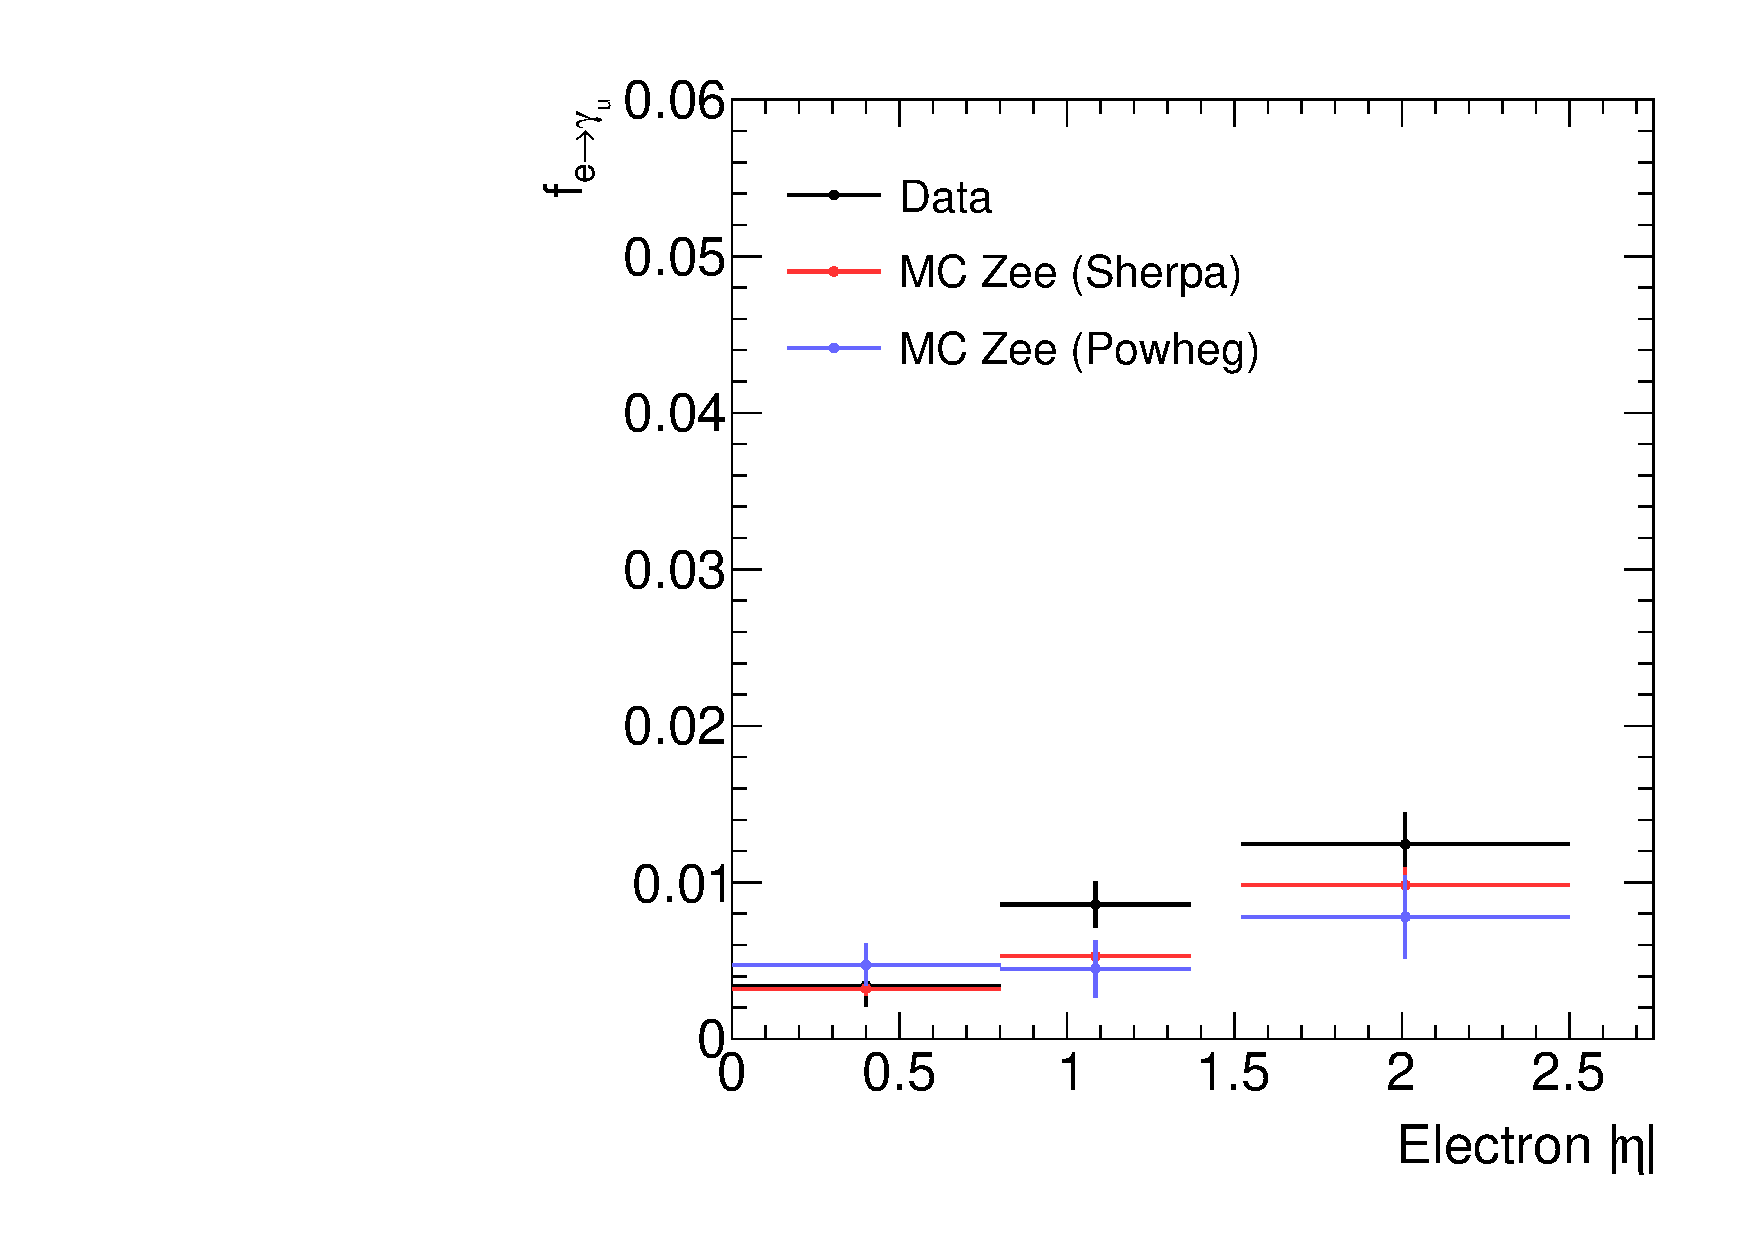
\includegraphics[width=0.45\textwidth]{figures/fegu_feta}

  \caption{Probabilidad de que un electrón real sea identificado como un fotón convertido (izquierda)
    y un fotón no-convertido (derecha), como función de la pseudo-rapidez del objeto \emph{probe}. El valor
    calculado a partir de los datos es comparado con el valor calculado con las muestras MC de eventos de {\Zee} utilizando
    dos generadores distintos.}
  \label{fig:efake_eta}
\end{figure}


\begin{table}[!htb]
  \centering
  \caption{Probabilidad de que un electrón real sea identificado como un fotón
    como función de la pseudo-rapidez del objeto \emph{probe}. El valor
    calculado a partir de los datos es comparado con el valor calculado con las
    muestras MC de eventos de {\Zee} utilizando dos generadores distintos.}
  \label{tab:efake_eta}

  \begin{tabularx}{0.9\textwidth}{CCCC}
    \hline
                          & Datos             &  MC {\Zee} (\sherpa) & MC {\Zee} (\powheg) \\
    \hline
    $0 < |\eta| < 0.8$    & $0.014 \pm 0.002$ & $0.012 \pm 0.001$ & $0.014 \pm 0.002$ \\
    $0.8 < |\eta| < 1.52$ & $0.018 \pm 0.003$ & $0.014 \pm 0.001$ & $0.011 \pm 0.003$ \\
    $1.52 < |\eta| < 2.5$ & $0.033 \pm 0.006$ & $0.027 \pm 0.002$ & $0.032 \pm 0.006$ \\
    Inclusivo             & $0.019 \pm 0.001$ & $0.016 \pm 0.001$ & $0.017 \pm 0.002$ \\
    \hline
  \end{tabularx}

\end{table}

\begin{table}[!htb]
  \centering
  \caption{Probabilidad de que un electrón real sea reconstruido como un fotón
    convertido ($f_{e\to \gamma_c}$) o no-convertido ($f_{e\to \gamma_u}$).
    El valor calculado a partir de los datos es comparado con el valor calculado
    con las muestras MC de eventos de {\Zee}, utilizando dos generadores distintos.}
  \label{tab:efake_uc}

  \begin{tabularx}{0.9\textwidth}{CCCC}

    \hline
                       & Datos              & MC {\Zee} (\sherpa)        & MC {\Zee} (\powheg)        \\
    \hline
    $f_{e\to \gamma_u}$ & $0.007 \pm 0.001$ & $0.005 \pm 0.001$ & $0.005 \pm 0.001$ \\
    $f_{e\to \gamma_c}$ & $0.013 \pm 0.001$ & $0.011 \pm 0.001$ & $0.011 \pm 0.002$ \\
    $f_{e\to \gamma}$   & $0.019 \pm 0.001$ & $0.016 \pm 0.001$ & $0.017 \pm 0.002$ \\
    \hline
  \end{tabularx}

\end{table}


Para estimar la incerteza sistemática del método utilizado, el factor {\feg} fue
calculado variando el tamaño de la ventana de masa del $Z$, y sin la sustracción
del fondo. Como se aprecia en la \cref{tab:efake_syst} la mayor variación se
obtine en el caso de no realizar la sustracción del fondo y por lo tanto se
utiliza este valor como la incerteza sistemática del método, a pesar de que
resulta el límite más desfavorable.

\begin{table}[!htb]
  \centering
  \caption{Probabilidad de que un electrón real sea reconstruido como un fotón
    convertido o no-convertido, para variaciones del método original.}
  \label{tab:efake_syst}

  \begin{tabularx}{0.9\textwidth}{CCCC}
    \hline
            &  $m_{ee} \in [71, 111] \GeV$ & $m_{ee} \in [86,96] \gev$ & Sin sustracción del fondo  \\
    \hline
    $f_{e\to \gamma_u}$ & $0.007 \pm 0.001$ & $0.007 \pm 0.001$ & $0.012 \pm 0.001$ \\
    $f_{e\to \gamma_c}$ & $0.013 \pm 0.001$ & $0.012 \pm 0.001$ & $0.012 \pm 0.001$ \\
    $f_{e\to \gamma}$   & $0.019 \pm 0.001$ & $0.019 \pm 0.001$ & $0.024 \pm 0.001$ \\
    \hline
  \end{tabularx}

\end{table}


El valor calculado del factor de identificación errónea de electrón en fotón
({\feg}) resulta entonces el que se muestra en la \cref{tab:efake_final}.

\begin{table}[!htb]
  \centering

  \caption{Probabilidad de que un electrón real sea reconstruido como un fotón {\feg}, como función de $\eta$, junto
    con su incerteza estadística y sistemática.}
  \label{tab:efake_final}

  \begin{tabularx}{0.75\textwidth}{CC}

    \hline
     Región                &  $f_{e\to \gamma}$  \\
    \hline
      $0 < |\eta| < 0.8$     & $  0.014 \pm 0.002 \stat\ \pm 0.005 \syst\ $ \\
      $0.8 < |\eta| < 1.52$  & $  0.018 \pm 0.003 \stat\ \pm 0.004 \syst\ $ \\
      $1.52 < |\eta| < 2.5$  & $  0.033 \pm 0.006 \stat\ \pm 0.008 \syst\ $ \\
    \hline
  \end{tabularx}

\end{table}


En la {\SRL} se observaron 28 eventos que pasaban la selección al invertir el
rol de fotón y electrón, lo que corresponde a una estimación del fondo de
$N^{\SRL}_{e\to\gamma} = 0.38\, \pm\, 0.10$. En {\SRH}, dado el alto corte en
{\met}, no se observó ningún evento en la muestra de electrones.



%-----------
% Jet fakes
%-----------
\section{Jets identificados como fotones}
\label{sec:jfakes}

Los jets pueden ser identificados como fotones si tienen uno o dos {\pizero} con
alto {\pt} como partícula \emph{leading}, resultando en un objeto
electromagnético indistinguible de un fotón muy energético. Este fondo
proviene mayoritariamente de multijets, {\wjets} y eventos {\ttbar} decayendo
semi-leptónicamente, y puede ser una fuente importante de contaminación debido a
la gran sección eficaz de producción de estos procesos. Como la proporción de
jets mal identificados como fotones no está bien descripta por el MC, se
utiliza un método especialmente desarrollado a partir de los datos para su estimación.
La idea consiste en utilizar las diferencias en la distribución de energía de aislamiento
esperada para fotones reales y falsos, como se describe a continuación.

\subsection{Descripción del método}

Para reducir significativamente el fondo proveniente de jets, en el análisis se
utilizan fotones que satisfacen un criterio de selección \emph{tight}, como se
describe en \cref{sec:obj_photons}. Esta selección es inclusiva respecto a los
fotones reales, tiene una moderada contaminación de jets y es, por definición,
un criterio más ajustado que el trigger de fotones utilizado para la toma de los
datos. Por esta razón, hay una suficiente cantidad de candidatos a fotones
provenientes de jets que fallan la selección \emph{tight} pero satisfacen una
selección intermedia. Estos jets más similares a un fotón real, denominados
\emph{pseudo-fotones}, son útiles para modelar los jets que pasan la selección
total y la fracción de esta contaminación.

%Pseudo-photons are here defined as those passing the loose identification
%but failing (at least) one of a set of tight identification cuts. %, also known as {\it loose'-non-tight}.

La muestra de fotones que pasan los criterios de selección \emph{tight}
($N_{tight}$) contiene, en general, fotones reales ($N_{\gamma}$) y falsos
($N_{j\to\gamma}$), es decir, $N_{tight} = N_{\gamma} + N_{j\to\gamma}$.
Las distribuciones de la energía de aislamiento para estas
dos contribuciones van a tener formas diferentes, lo que puede ser explotado
para estimar ambas contribuciones. Para tal fin, se ajusta la distribución
total de energía de aislamiento con un combinación de modelos de señal y fondo.

El número de eventos de fotones falsos que pasa la identificación de fotones y
el corte de aislamiento puede ser estimado entonces integrando la componente de
fondo del ajuste sobre el rango de la región de señal ($\etiso<5\GeV$). De esta
forma la proporción de jets mal identificados como fotones, \fjg, resulta:

\begin{equation}\label{eq:jfake_formula}
  f_{j\to \gamma} = \frac{\int_{-\infty}^{5\gev} B(x)\, dx}{\int_{-\infty}^{5\gev} \left[S(x)+B(x)\right]\, dx}
\end{equation}
%
donde $x$ es la variable de energía de aislamiento \etiso, y $S(x)$ y $B(x)$ son
las distribuciones de señal y fondo en el ajuste combinado, respectivamente.
Esta fracción de fotones falsos es estimada en una región lo más cercana posible
a las regiones de señal, y luego utilizada para estimar el número de eventos
provenientes de jets mal identificados, pesando la muestra de fotones en la SR.




\subsection{Modelo de Señal} \label{sec:jfake_sig_template}

El modelo de señal se extrajo a partir de electrones provenientes de eventos de datos {\Zee}
utilizando el hecho que los
electrones y fotones dejan una señal similar en el calorímetro
electromagnético. La muestra de electrones es obtenida de eventos que satisfacen
el siguiente conjunto de cortes, después de haber pasado la preselección
descripta en \cref{sec:preselection}:

\begin{itemize}\itemsep0.1cm
\item Trigger de electrones %% (\texttt{2e12Tvhi\_loose}, \texttt{e24vhi\_medium} o \texttt{e60\_medium}).
\item Dos electrones \emph{medium}, aislados, con carga opuesta, y con $\pt>50,25\gev$
\item \MET\ $<40\gev$
\item $81\gev<m_{ee}<101\gev$
\end{itemize}

Después de aplicar los cortes anteriores, la contaminación de fondos no
provenientes del decaimiento del $Z$ es despreciable y, en particular, para eventos
de {\ttbar} resulta menor al $1\%$.

\begin{figure}[!htb]
  \centering

  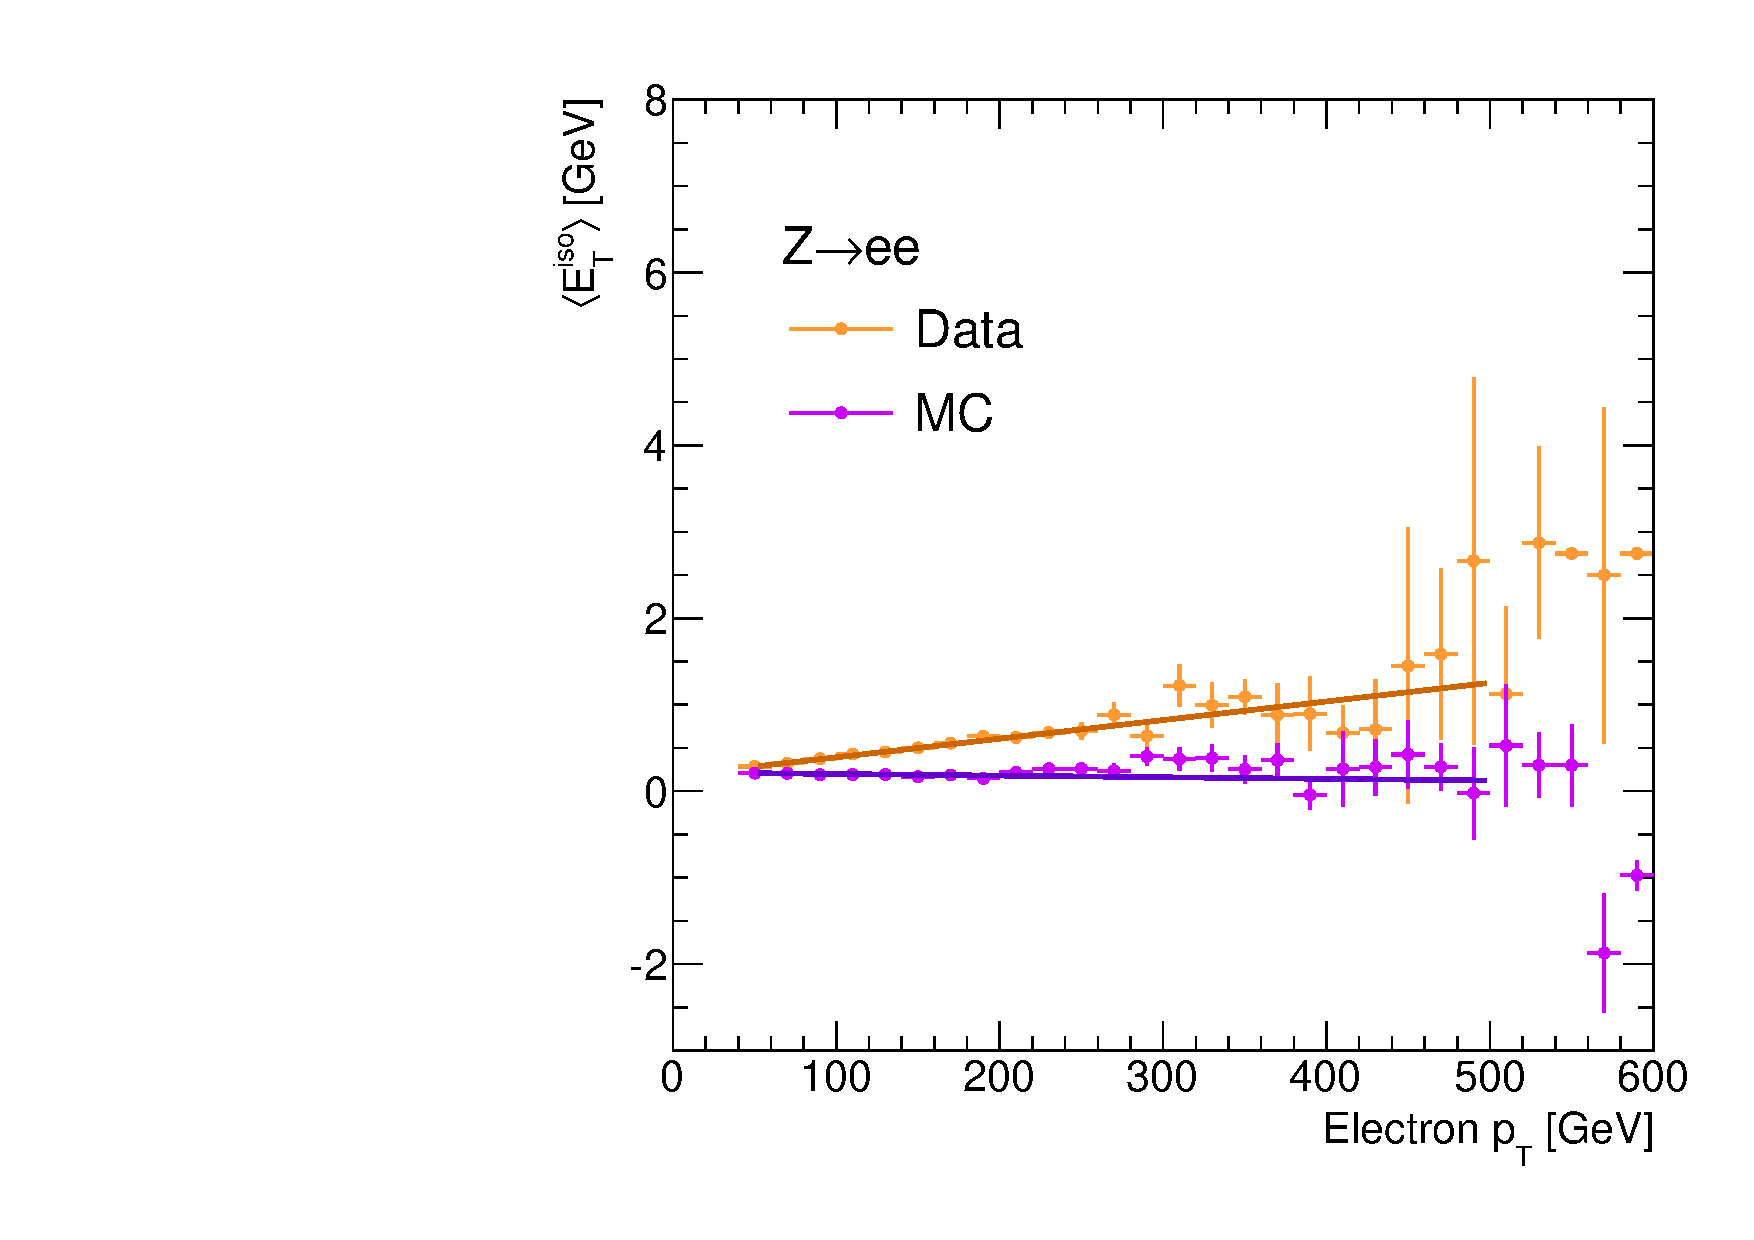
\includegraphics[width=0.49\textwidth]{electron_iso_vs_pt_Zee_raw}

  \caption{Distribución de la energía de aislamiento ({\etiso}) de electrones provenientes
    de eventos {\Zee} en datos y MC, en función de {\pt}.}
  \label{fig:isolation_vs_pt}
\end{figure}

La \cref{fig:isolation_vs_pt} muestra el valor medio de la distribución de la energía de
aislamiento para los electrones seleccionados como función del {\pt} del
electrón en eventos de datos y simulaciones MC. De la figura resulta evidente que
para los datos existe una clara dependencia de {\etiso} con {\pt}, que no es el caso
para las simulaciones MC.
Para corregir esta dependencia residual con {\pt} se realiza un ajuste lineal de los
datos del cual se obtiene un factor de corrección que luego es aplicado a {\etiso}.
El valor del factor de corrección
obtenido en el ajuste en el rango $50<\pt<500 \gev$ es $0.00262 \pm 0.00008$.

En la \cref{fig:isolation_wandwo_correction} se muestra una comparación entre
datos y simulaciones del perfil de {\etiso} antes y después de la corrección. Se
puede ver que el acuerdo entre datos y MC es mucho mejor después de aplicar la
corrección.


\begin{figure}[!htb]
  \centering

  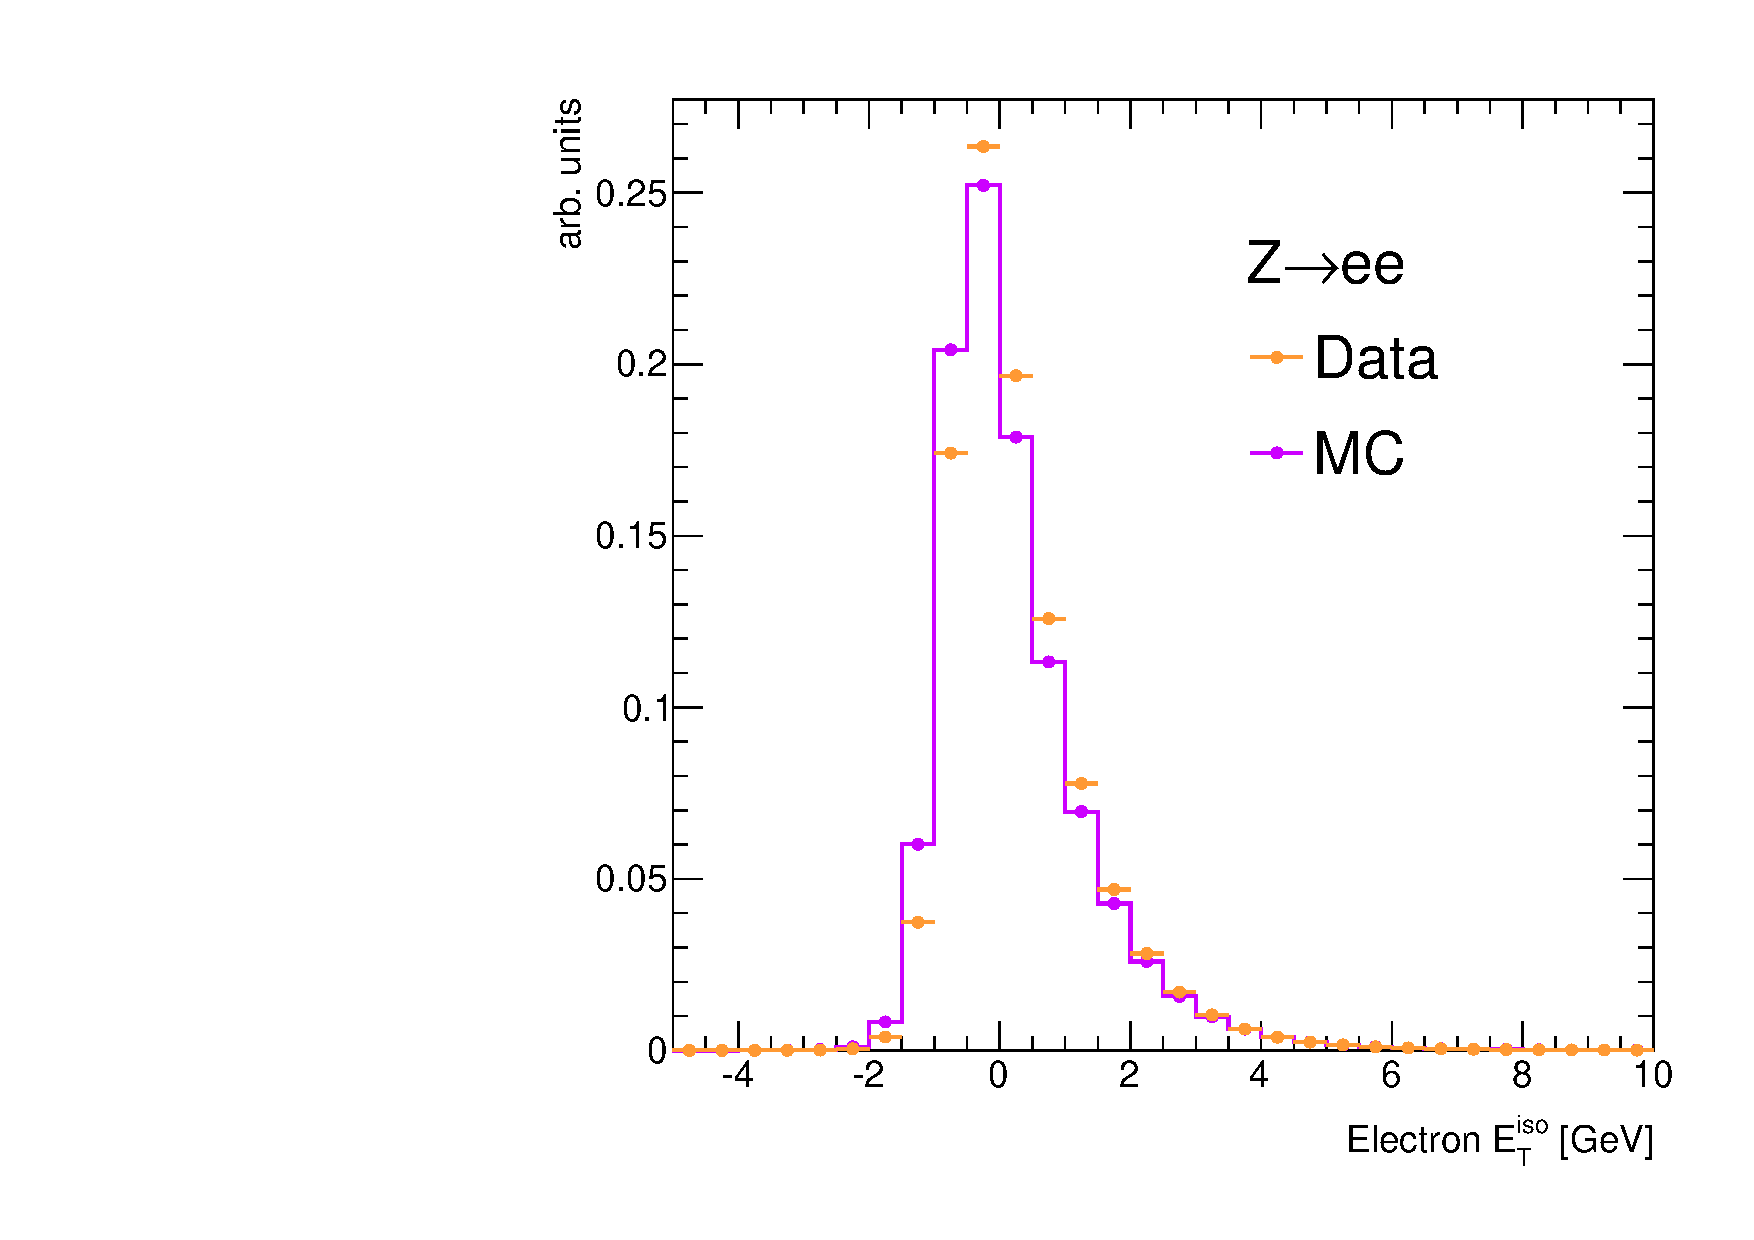
\includegraphics[width=0.49\textwidth]{electron_iso_Zee_raw}
  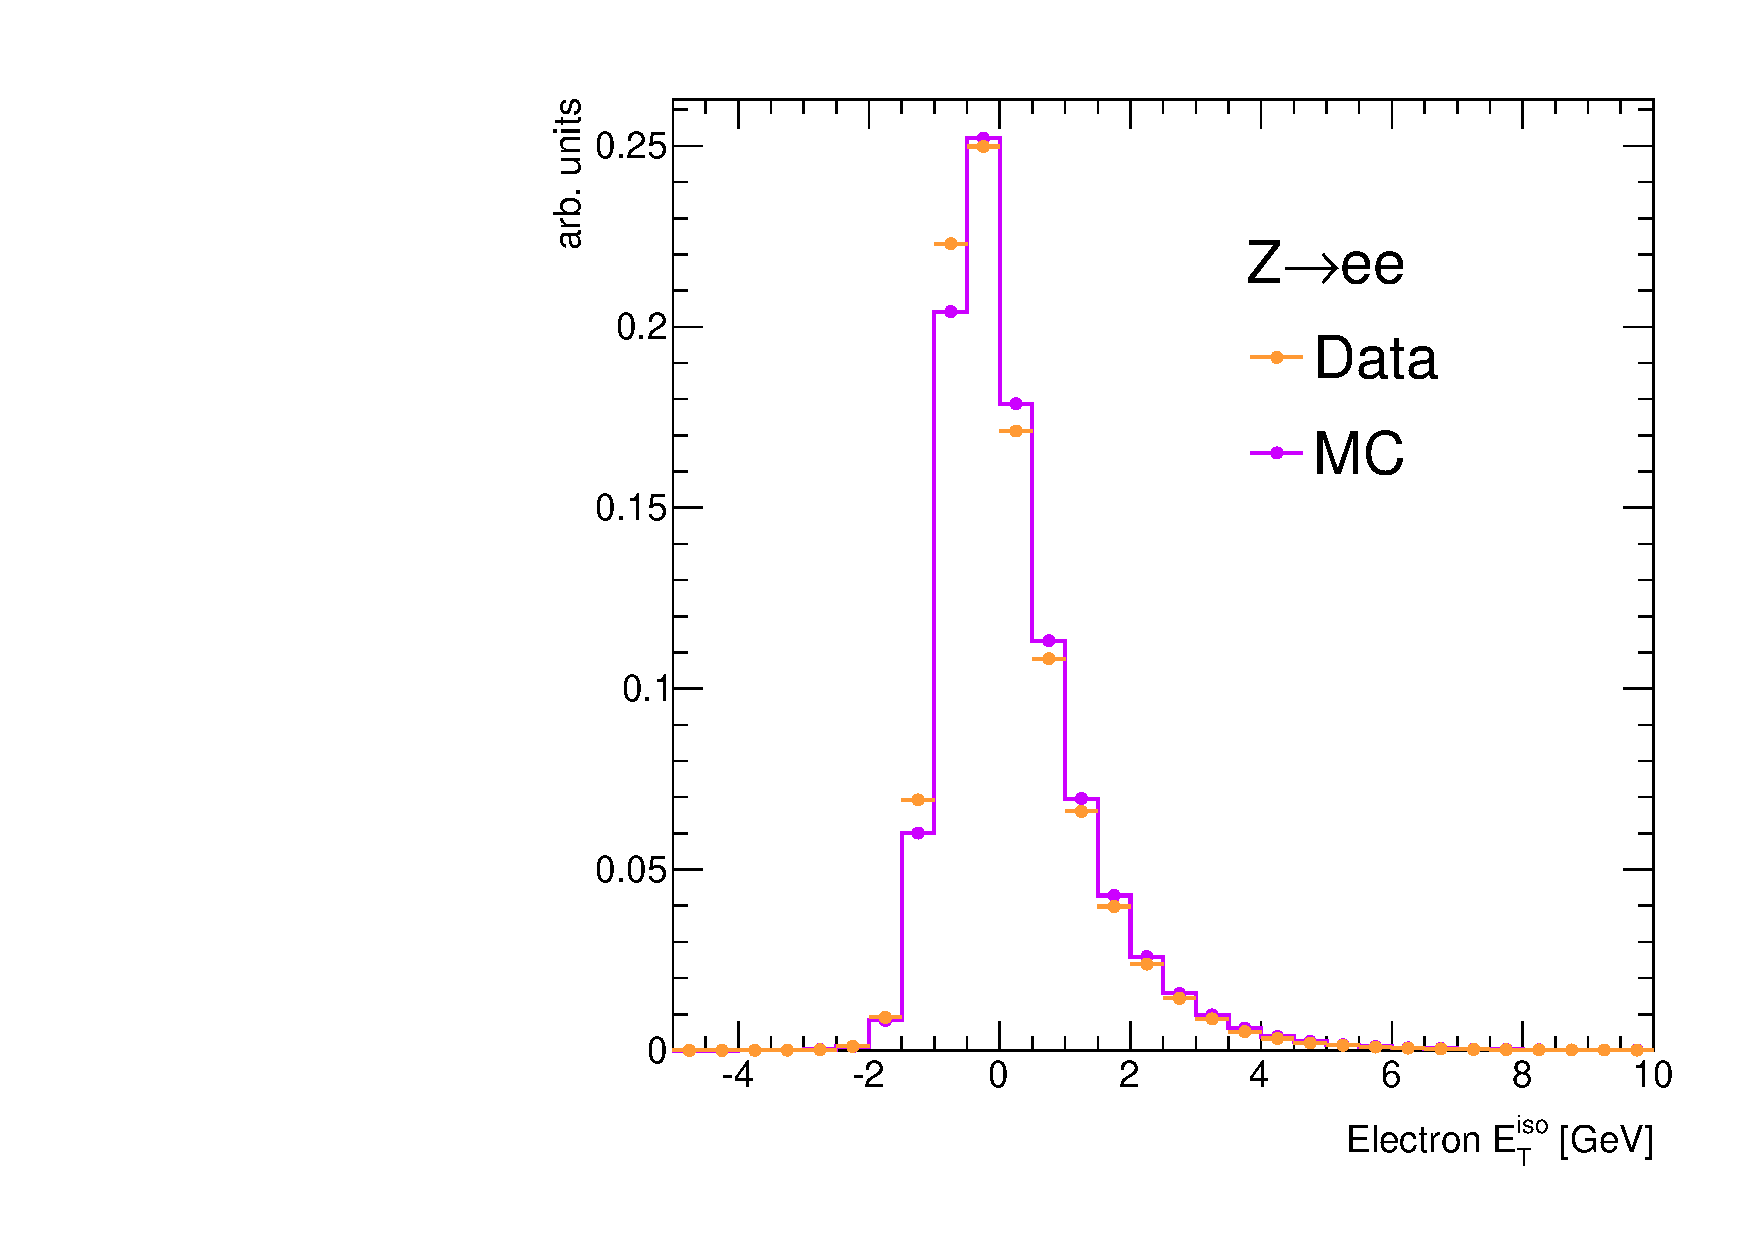
\includegraphics[width=0.49\textwidth]{electron_iso_Zee_corr}

  \caption{Comparación datos/MC de la distribución de {\etiso} de electrones
    provenientes de eventos {\Zee} (izquierda) y la correspondiente distribución
    después de aplicar la corrección por el {\pt} (derecha).}
  \label{fig:isolation_wandwo_correction}
\end{figure}

Para respaldar la estrategia de derivar el modelo de aislamiento de los fotones
a partir de electrones se realizaron varios estudios. Una validación importante
del método consistió en comparar la distribución de {\etiso} de electrones
provenientes de {\Zee} con los fotones provenientes del decaimiento radiativo
del $Z$ (\Zee\gam) que provee un fuente de fotones puros. Los eventos se
seleccionaron requiriendo el siguiente conjunto de cortes, después de la
preselección:

\begin{itemize}\itemsep0.1cm
\item Triggers de electrones %%(\texttt{2e12Tvhi\_loose1} o \texttt{e24vhi\_medium1} o \texttt{e60\_medium1})
\item Un fotón \emph{tight} aislado con $\pt>25 \gev$.
\item Dos electrones \emph{medium}, aislados, con carga opuesta, y con $\pt>50 \gev$ y $\pt>25 \gev$
\item $\Delta R(\gamma,l)>0.7$
\item \MET\ $<40\gev$
\item $40\gev<m_{ee}<85\gev$
\item $70\gev<m_{ee\gamma}<100\gev$
\end{itemize}

En la \cref{fig:photon_electron_iso} se presenta una comparación entre el modelo
de fotones reales de decaimientos radiativos del $Z$ y electrones de {\Zee}. El
gráfico a la derecha es obtenido después de remover la dependencia con el {\pt}
con el factor de corrección como se describió anteriormente. Puede verse, a partir
del cociente en el panel inferior,
el buen acuerdo entre las distribuciones de {\etiso} de fotones y
electrones, en particular después de aplicar la corrección, dando confianza en la
hipótesis de usar electrones para modelar los fotones.

%% Vale la pena nota que el espectro de {\pt} de fotones tan bajo en estos
%% procesos (ver {\fig} \ref{fig:zllg_pt}) as compared to the generally broader electron \pt\ spectrum from Z decay. %of the electrons (see {\fig} \ref{fig:zeeg_pt}). \tosolve{add this last plot}

\begin{figure}[!htb]
  \centering

  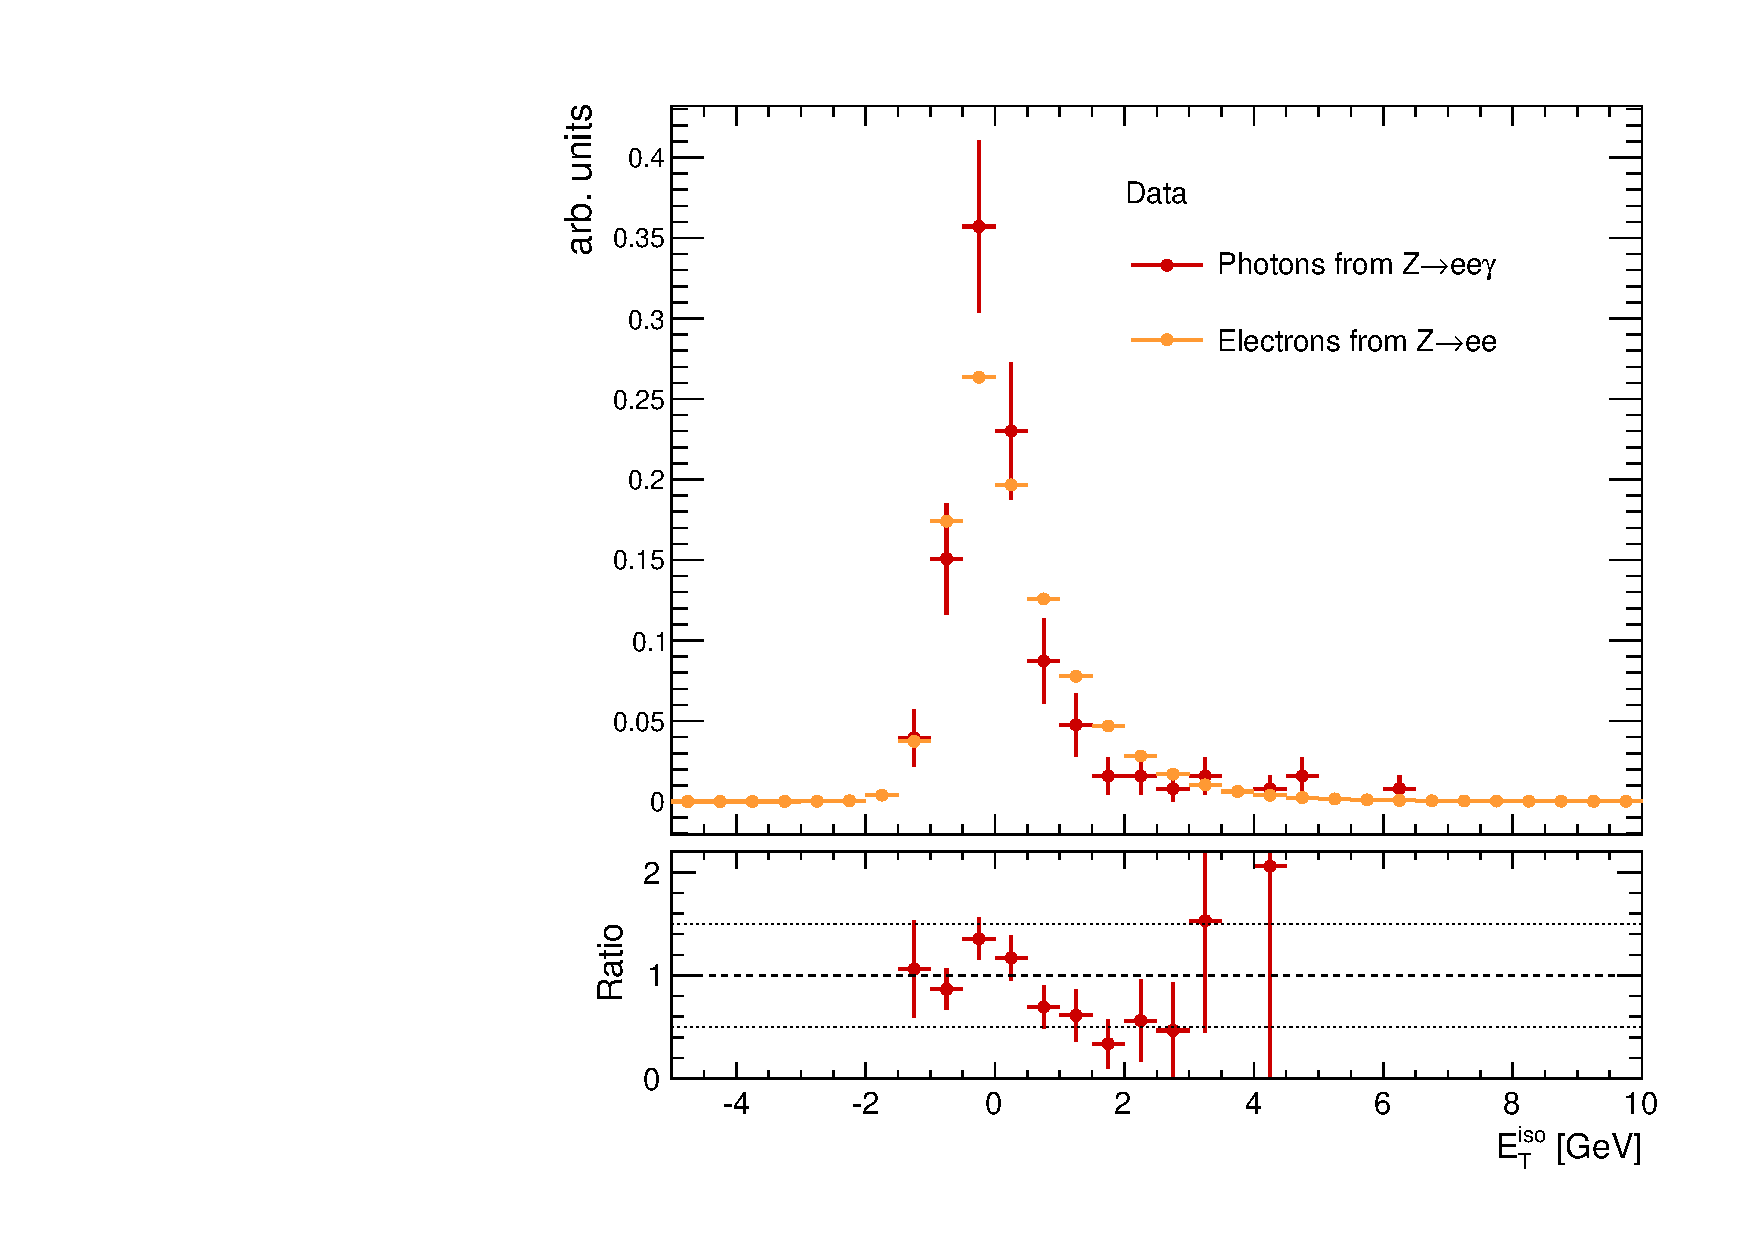
\includegraphics[width=0.49\textwidth]{electronphoton_iso_Zee_before_correction}
  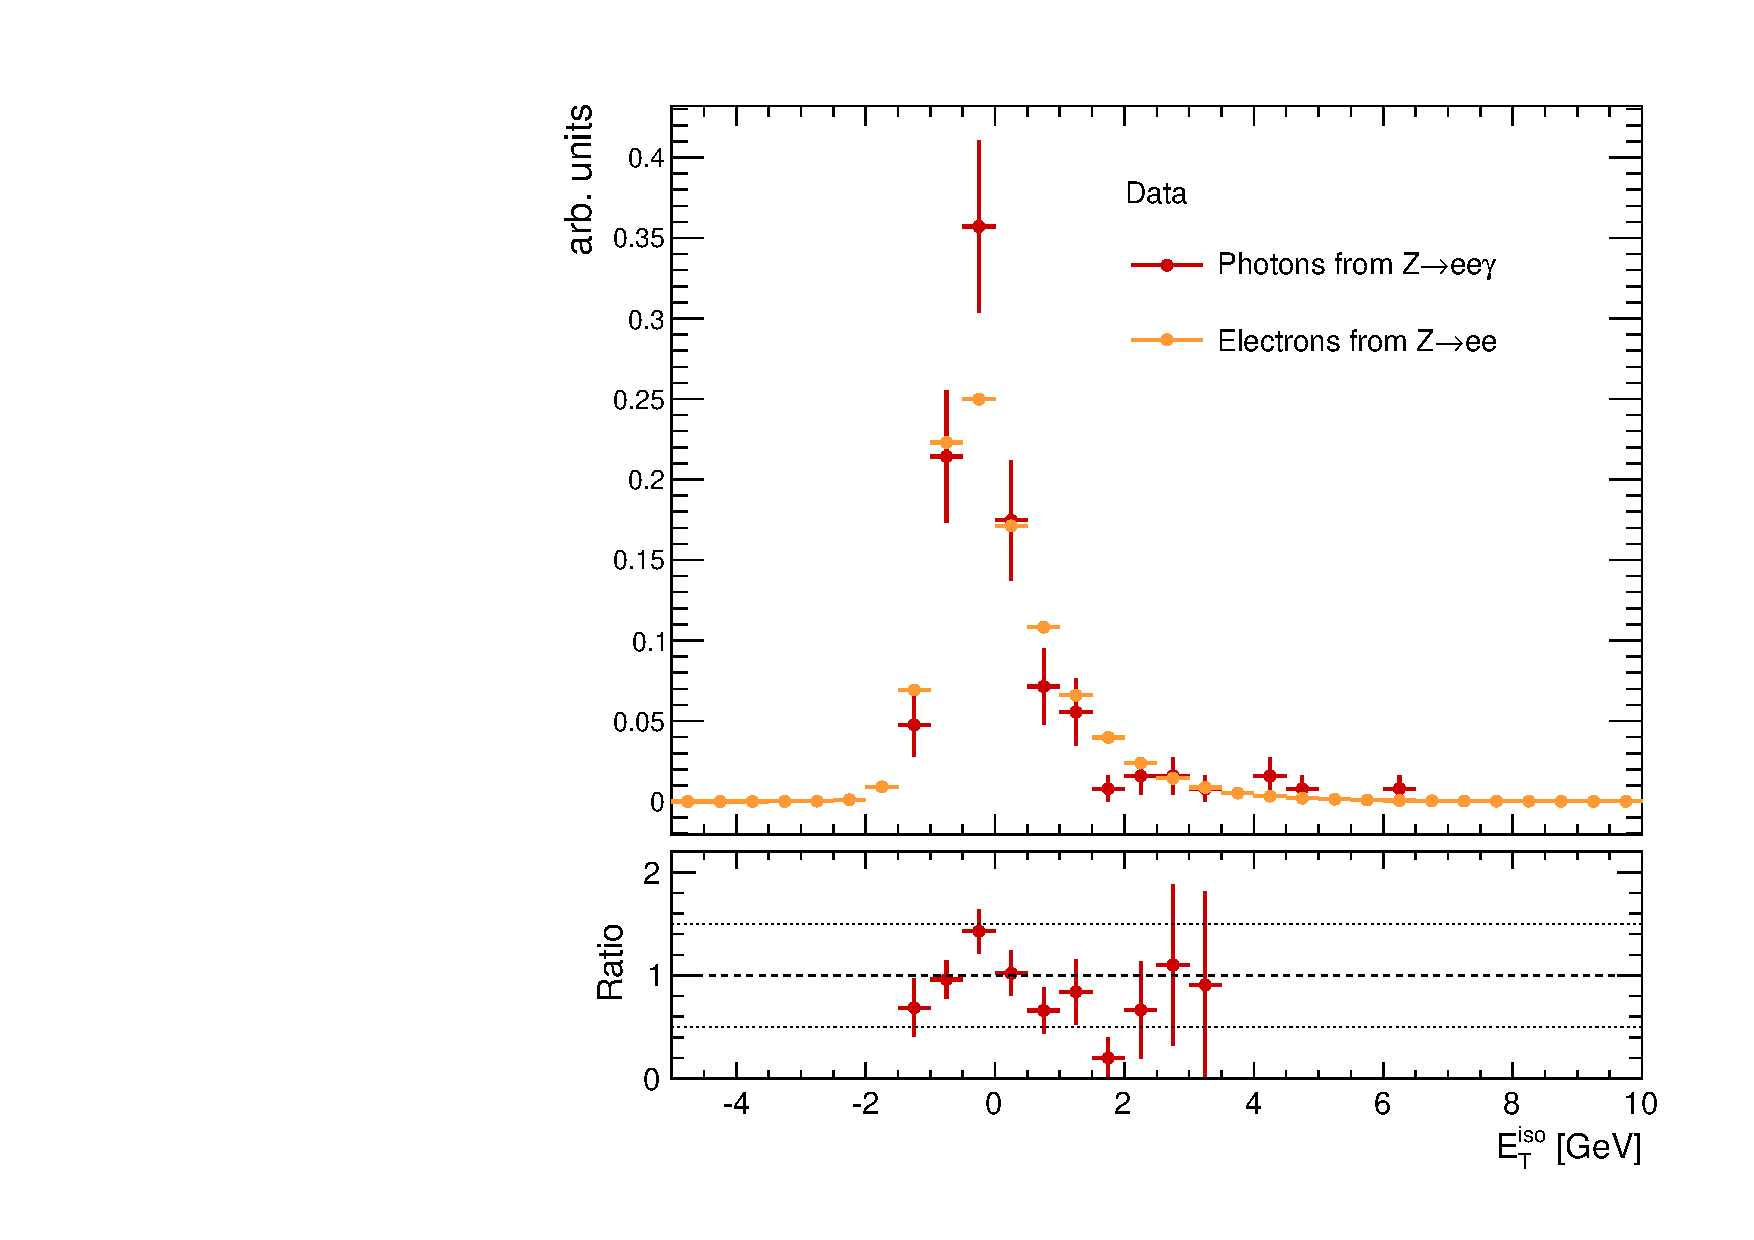
\includegraphics[width=0.49\textwidth]{electronphoton_iso_Zee_after_correction}

  \caption{Comparación de las distribuciones de la energía de aislamiento para fotones reales de
    decaimiento radiativo del $Z$ y electrones provenientes del decaimiento $\Zee$ antes (izquierda)
    y después (derecha) de la corrección por \pt.}
    \label{fig:photon_electron_iso}

\end{figure}

Para estudiar el efecto en las distribuciones obtenidas de {\Zee} en distintas
regiones cinemáticas, en la \cref{fig:electron_iso_HT}, se presentan las
distribuciones agregando un corte en {\HT} para eventos {\Zee} en muestras MC y
datos. Como es de esperar, la energía de aislamiento es más alta y la
distribución se hace más ancha con \HT. Desafortunadamente, la escasa
estadística impide el uso del corte en {\HT} de la SR. En cualquier caso, el
efecto se considera como una posible fuente de incerteza sistemática.

\begin{figure}[!htb]
  \centering

  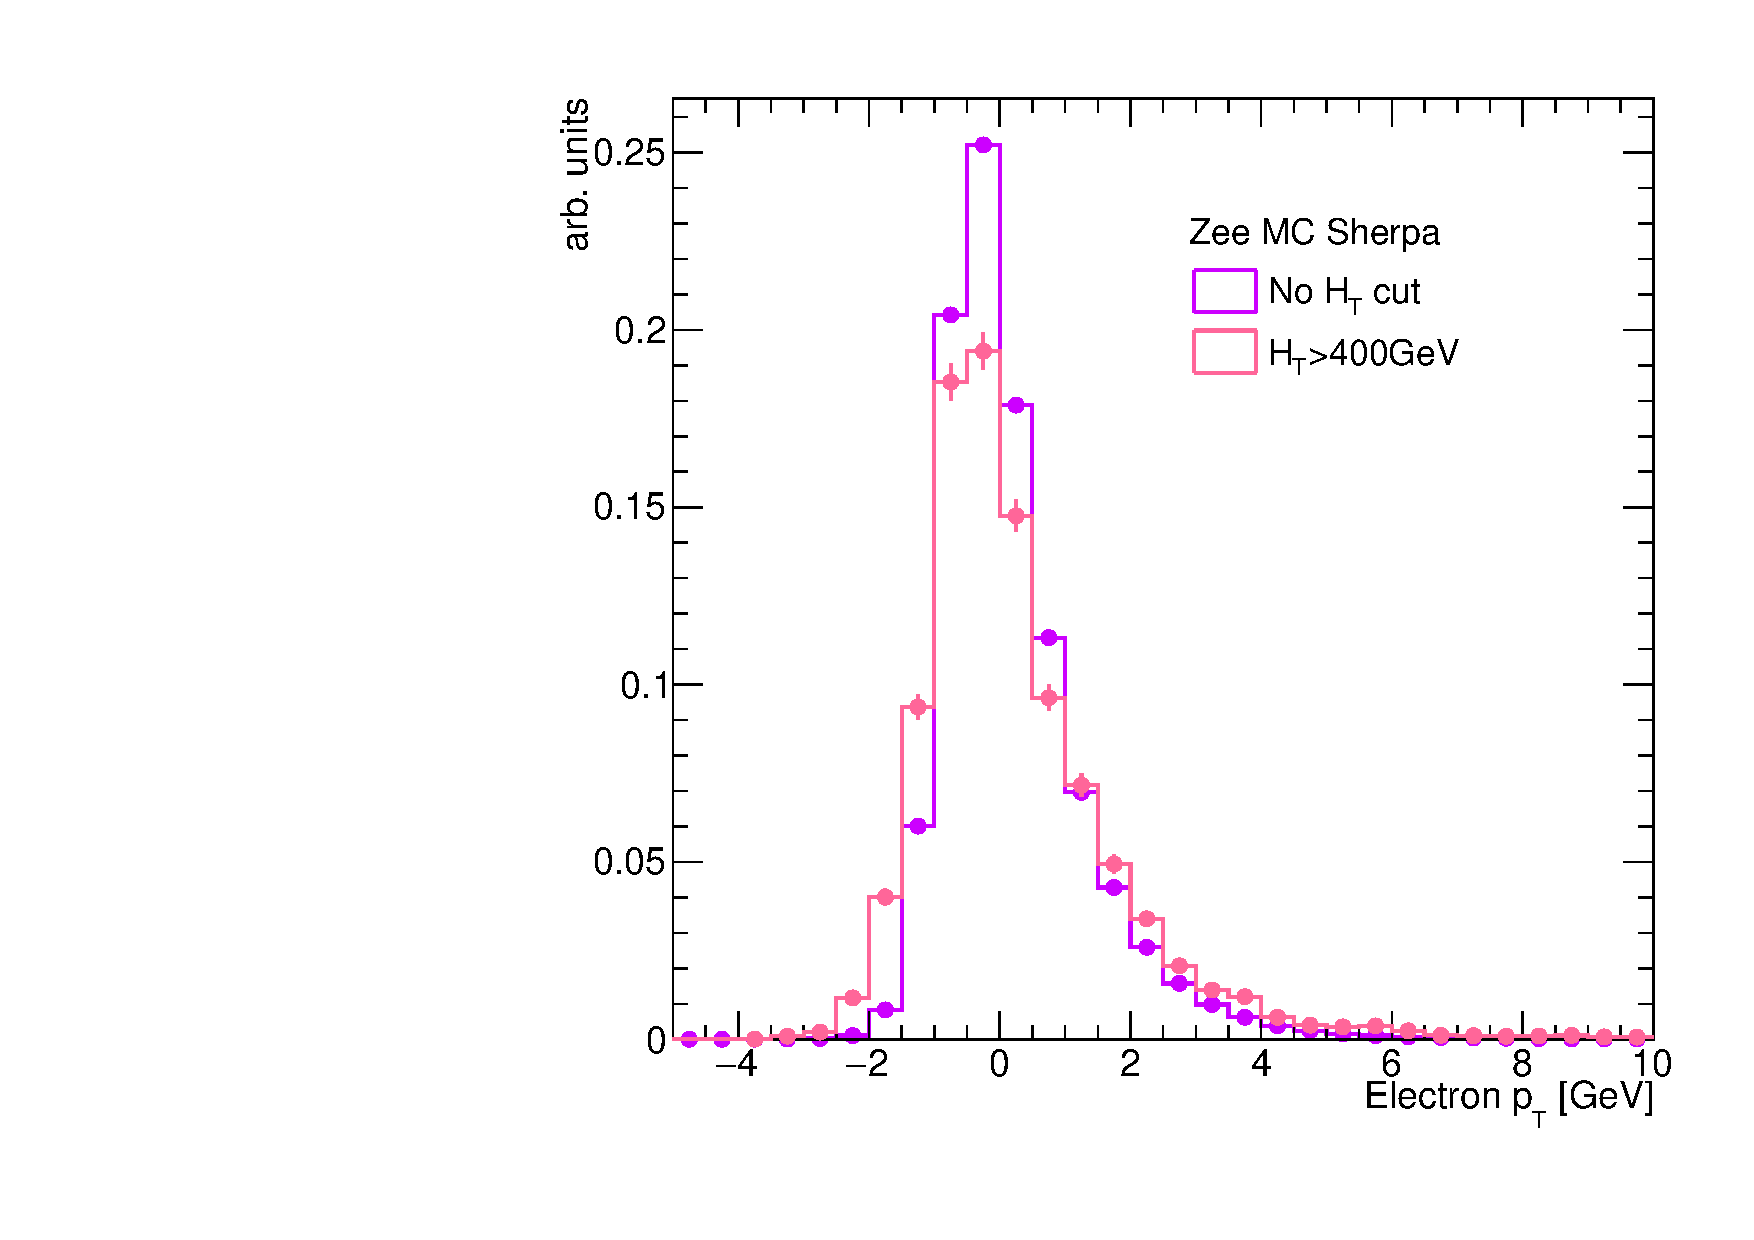
\includegraphics[width=0.49\textwidth]{electron_iso_ZeeHMC_corr}
  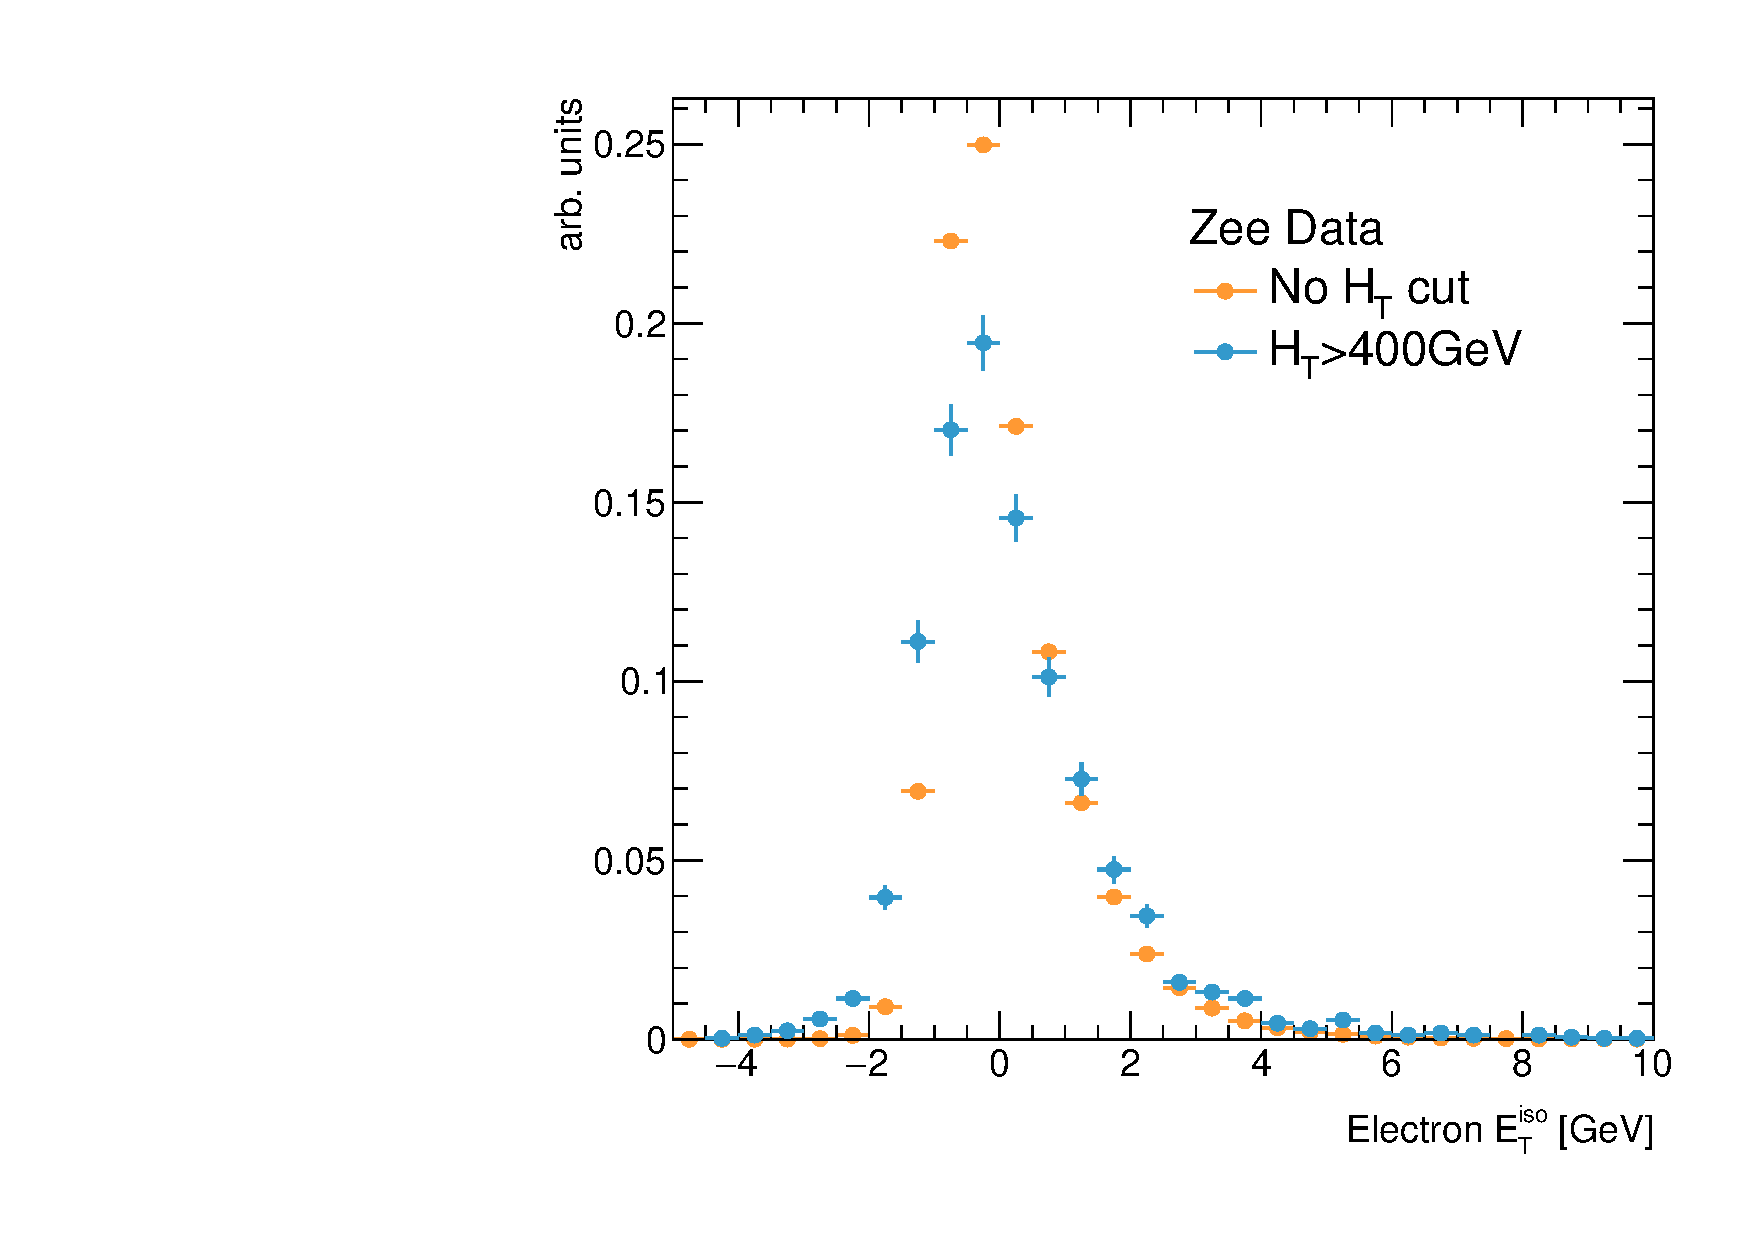
\includegraphics[width=0.49\textwidth]{electron_iso_ZeeH_corr}

  \caption{Dependencia de la energía de aislamiento de electrones con {\HT}
    para MC (izquierda) y datos (derecha) \Zee}
    \label{fig:electron_iso_HT}

\end{figure}



\subsection{Modelo de fondo} \label{sec:jfake_bkg_template}

El modelo de fondo se obtuvo de los datos, en eventos que pasan todos los
criterios de identificación salvo los criterios de identificación \emph{tight}
de fotones. La muestra de pseudo-fotones seleccionada de esta forma debe
presentar un perfil de aislamiento similar a la de fotones reales, permitiendo
una pequeña contaminación de señal y alta estadística.

Se realizó un estudio detallado en muestras MC para encontrar el mejor conjunto
de los cortes utilizados por el criterio de identificación \emph{tight} que debía ser
revertido para modelar de la mejor manera la distribución de aislamiento para
los fotones falsos provenientes de decaimientos de hadrones en la SR. En la
\cref{fig:jetfake_mc_data} se puede ver la comparación de dos definiciones
distintas de pseudo-fotones para MC y datos.
Los pseudo-fotones \emph{loose-non-tight} pasan los cortes de
identificación \emph{loose}, pero fallan al menos uno de los cortes
\emph{tight}. A pesar de la escasa estadística, resulta claro que falla en su
objetivo de modelar el fondo tanto en datos como en MC. Se obtiene un mejor
acuerdo para la definición \emph{loose'-non-tight}, en la cual los
fotones pasan todos los cortes \emph{tight} salvo (al menos) uno de las
variables en la sección de bandas del calorimetro ($F_\text{side}$, $w_{s3}$, $E_\text{ratio}$,
$\Delta E$). Estas variables son construidas con solo algunas bandas centrales
alrededor de la dirección del fotón, y por lo tanto se espera que no tengan una
correlación con la energía de aislamiento del fotón, ya que para el cálculo de
esta se excluye la energía en las celdas centrales para tener en cuenta la
propia energía del fotón. Utilizando esta definición, los pseudo-fotones tienen
un perfil de aislamiento con una forma similar a la de fotones \emph{tight} y
por lo tanto es posible la extrapolación a la SR.

\begin{figure}[!htb]
  \centering

  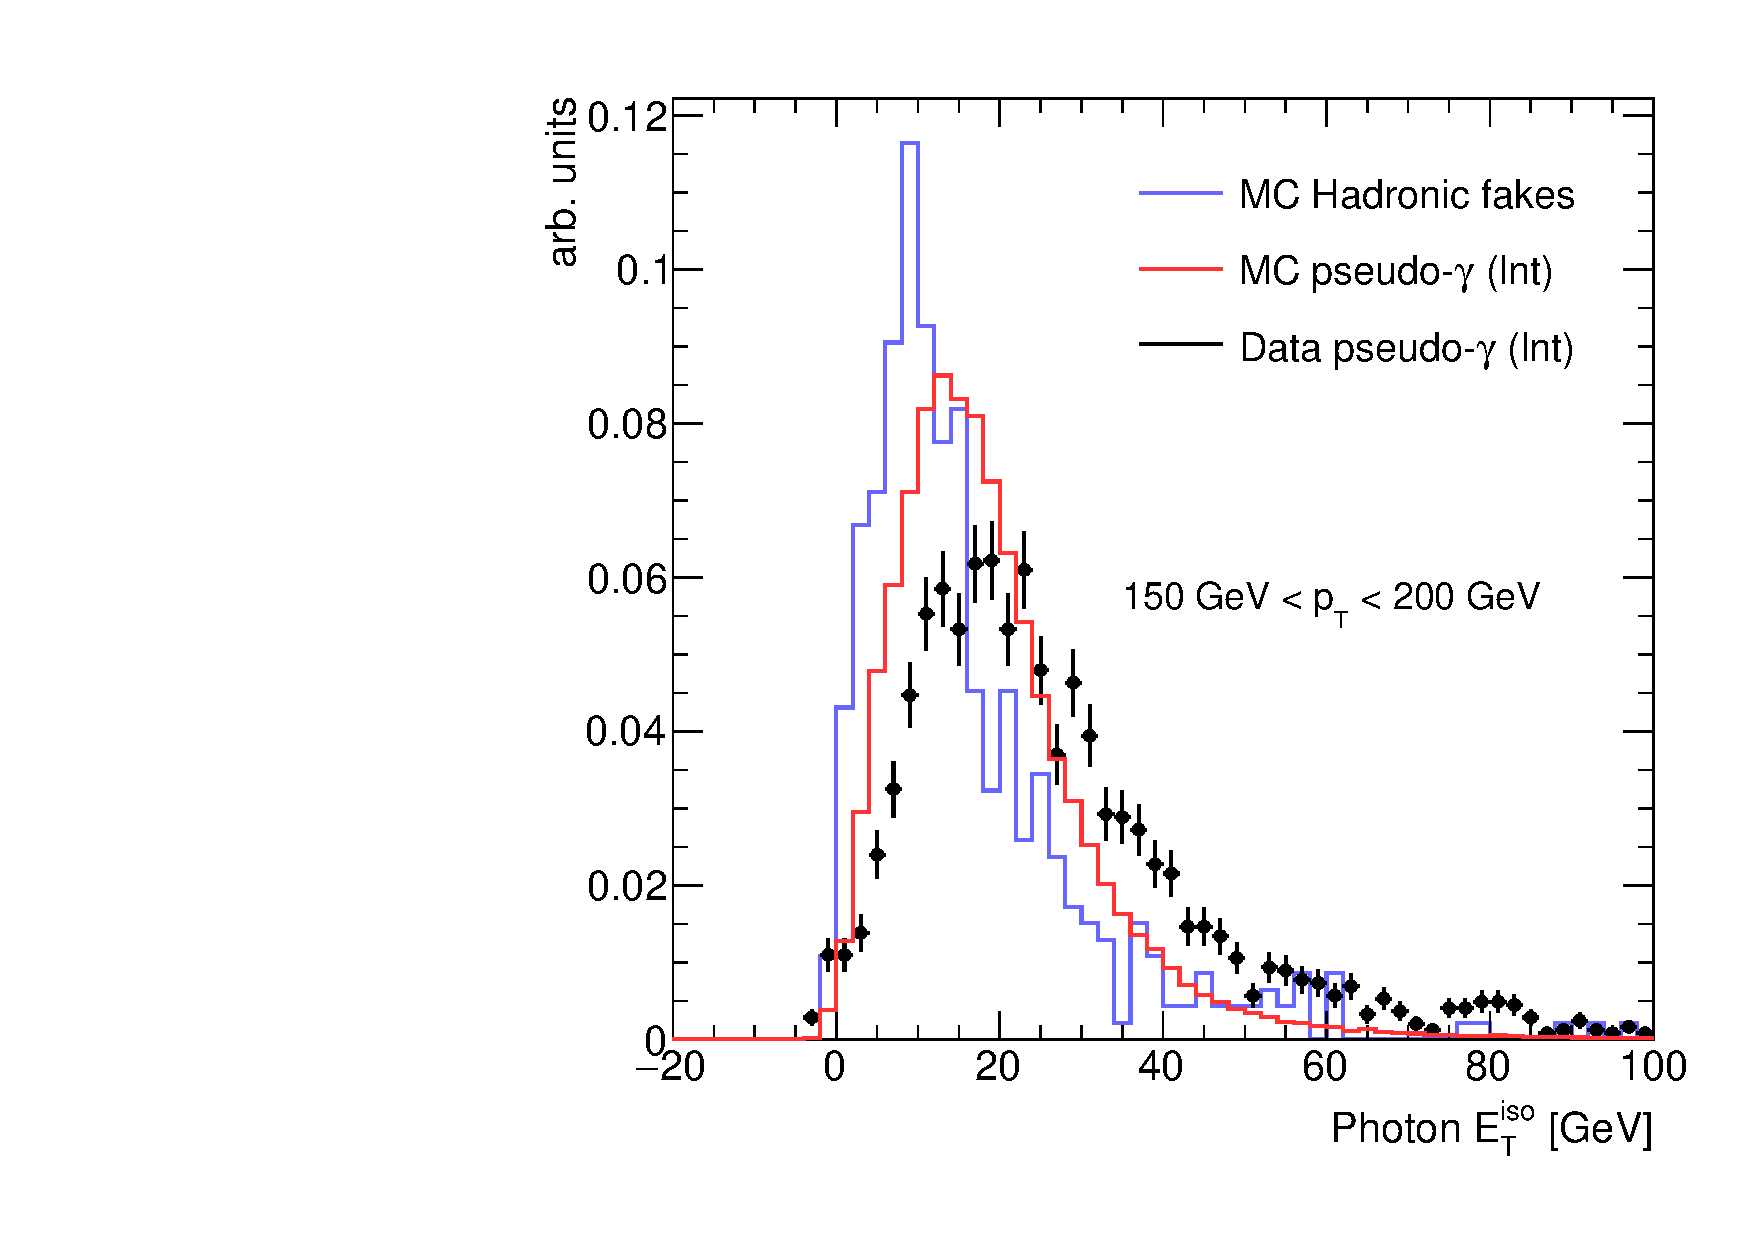
\includegraphics[width=0.49\textwidth]{figures/bkg_mc_pseudo_data_SR_l_ptbin}
  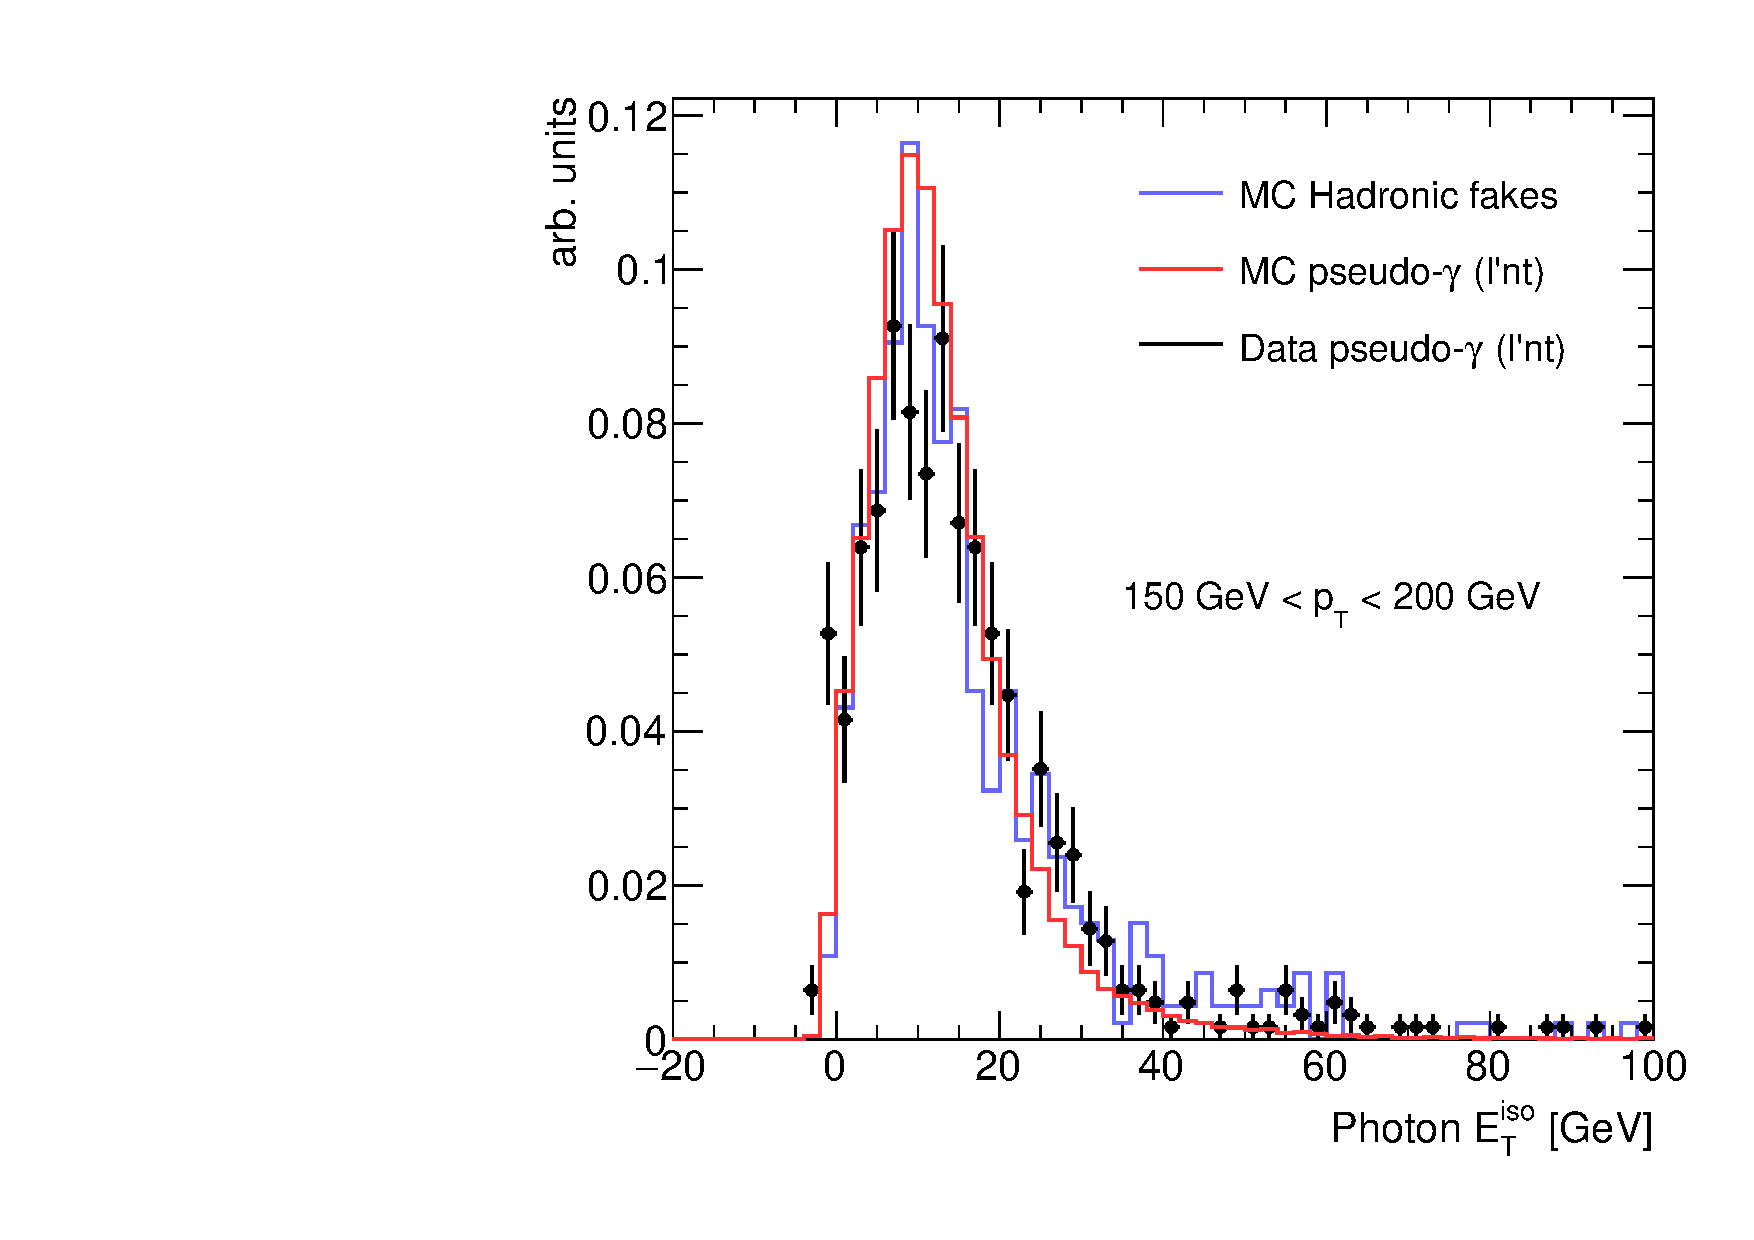
\includegraphics[width=0.49\textwidth]{figures/bkg_mc_pseudo_data_SR_lp_ptbin}

  \caption{Distribución de la energía de aislamiento para fotones falsos
    provenientes de decaimientos hadronicos (a nivel generador), comparada con
    la de pseudo-fotones obtenidos con dos definiciones diferentes: \emph{loose-non-tight} (izquierda)
    y \emph{loose'-non-tight} (derecha). Ver detalles en el texto.}
  \label{fig:jetfake_mc_data}

\end{figure}

Más aún, como se ve en la \cref{fig:jetfake_pseudo_data_pt}, los fotones \emph{loose'-non-tight}
reproducen mejor el espectro de {\pt} de los fotones \emph{tight}, y no es necesario
aplicar una correción por este motivo.

\begin{figure}[!htb]
  \centering

  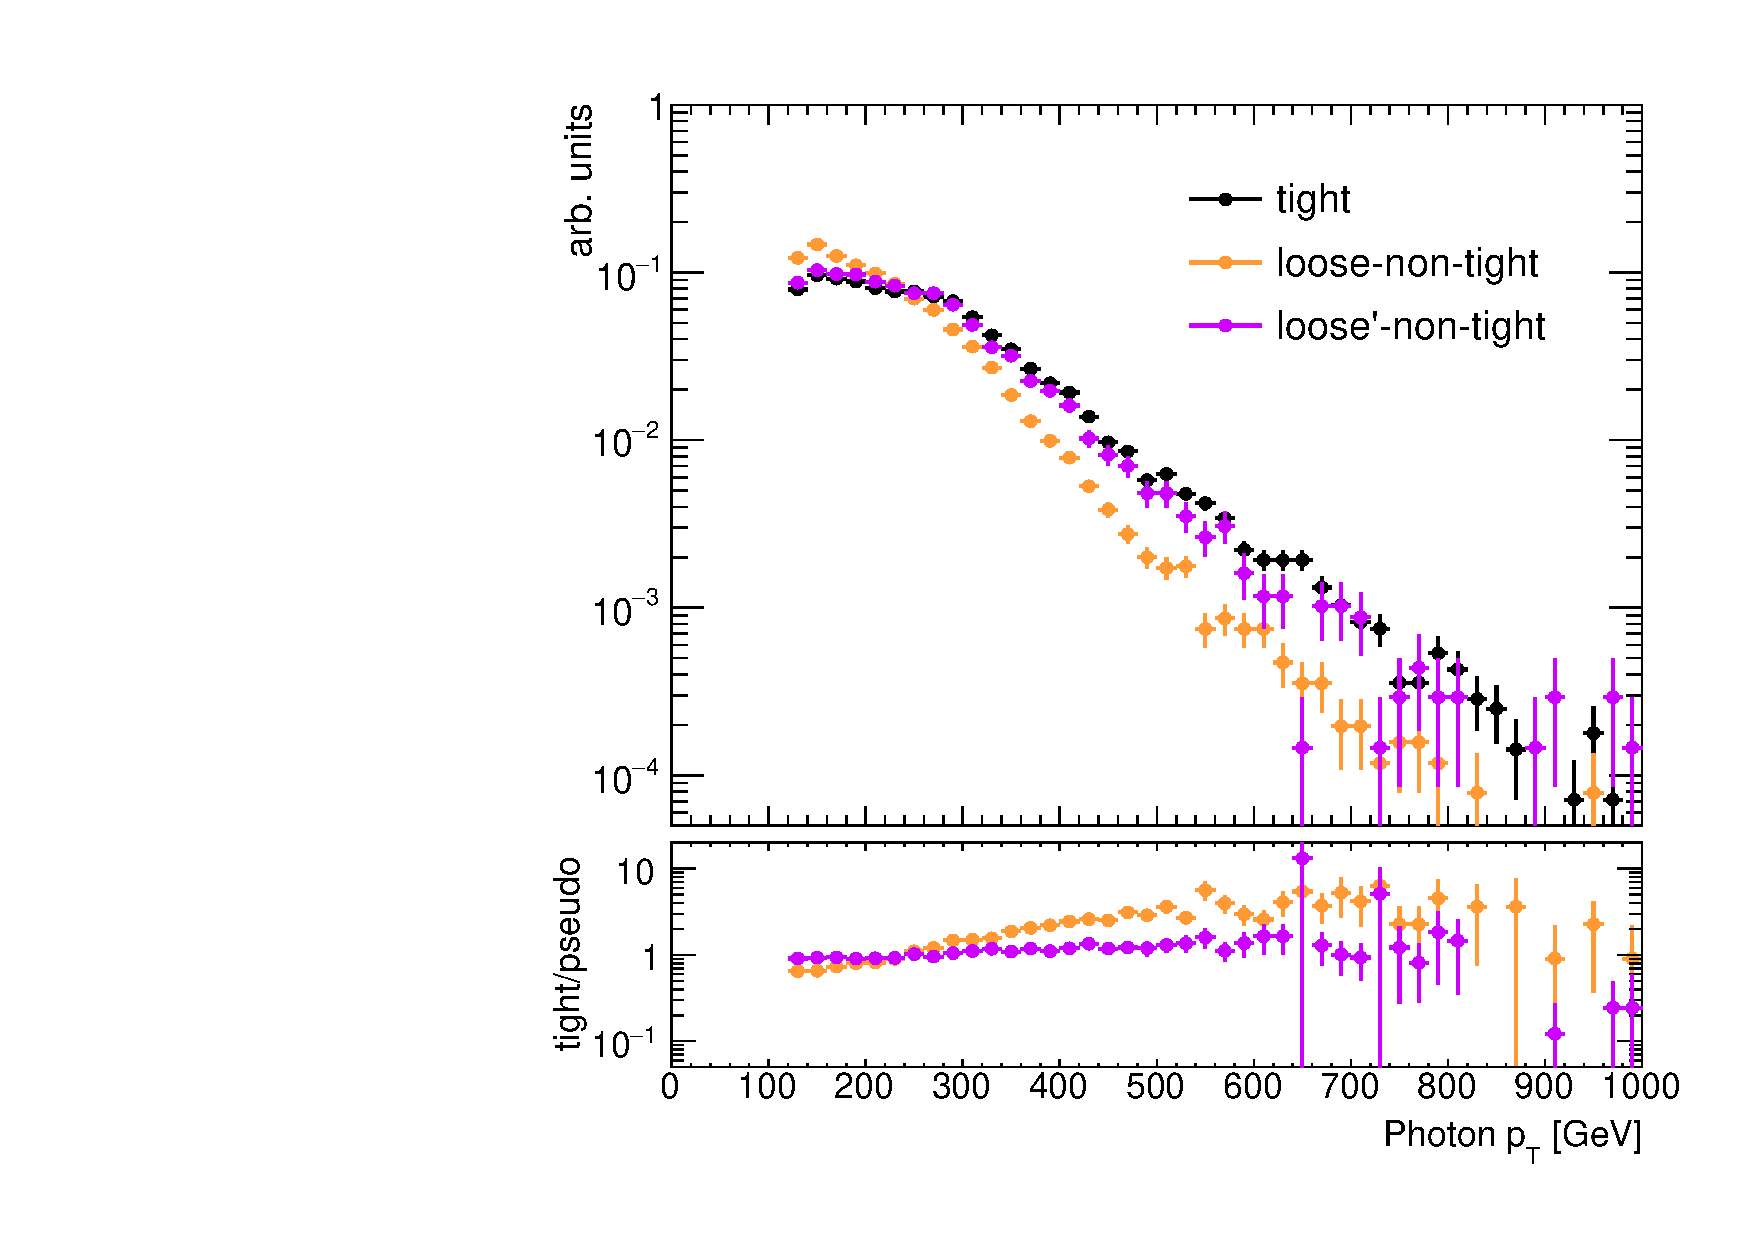
\includegraphics[width=0.5\textwidth]{bkg_data_pseudo_tight_data_VR}

  \caption{Distribución del {\pt} del fotón para candidatos
    \emph{tight} y las dos definiciones diferentes de pseudo-fotones.}
  \label{fig:jetfake_pseudo_data_pt}

\end{figure}


La distribución de la energía de aislamiento de los pseudo-fotones puede variar
en distintas regiones cinemáticas. Es por esta razón que para derivar el modelo
de fondo se utiliza una región relajada (CRJ), cercana a las regiones de señal, definida en
la \cref{tab:cr_jetfake}. Para mantener esta región ortogonal a las SR, se
requiere un corte intermedio en {\met}, y algunos otros cortes son relajados
para ganar estadística. Como se espera, a mayor actividad hadrónica en el
evento, mayor es la energía de aislamiento del fotón. En la
\cref{fig:jetfake_pseudo_data_LR_VR} se puede ver las diferencias para distintos
requerimientos en {\HT}. En la región CRJ se utiliza un corte intermedio entre
ambas SR, y las posibles diferencias son tenidas en cuenta como incerteza
sistemática.


%% For this reason, the control region selection to derive the templates is kept close to the SR, as listed in {\tab} \ref{tab:cr_jetfake}.
%% An orthogonality requirement is placed on \MET ($50-150\gev$) and some SR cuts are loosened to retain statistics.
%% As expected, however, the larger the jet activity around the harder the photon isolation in the event. So the
%% \HT\ requirements can not be loosened much. This can be clearly observed in {\fig} \ref{fig:jetfake_pseudo_data_LR_VR},
%% for a loose (CRFJL: $>200 \gev$) and tight (CRFJ: $>600 \gev$) \HT\ selection. The latter is therefore used to
%% perform the combined fit and to compute the jet fake factor, as discussed in the next section.

\begin{table}[!htb]
  \centering

  \caption{Definición de la region utilizada para la estimación de los jets mal identificados como fotones.}
  \label{tab:cr_jetfake}

%%   %%$f_{j\to\gamma}$ fake factor derived in the CRFJ region. The numeric suffix indicates (when present) the SR associated to each region (SR2 or SR3).}
  \begin{tabular}{rc}
    \hline
                                            &           CRJ  \\ %       CRFJL \\
    \hline
    $\pt(\text{pseudo}-\gamma)$ [\gev] $>$ &           125 \\ %         125 \\
    $\nleptons$                              &             0 \\ %           0 \\
    \met [\gev]                              &   $[50, 150]$ \\ % $[50, 150]$ \\
    $\njets \ge$                             &             2 \\ %           2 \\
    $\pt^{j_1,j_2}$  [\gev]  $>$             &           100 \\ %         100 \\
    $\dphijm >$                              &           0.4 \\ %         0.4 \\
    \HT [\gev] $>$                           &           600 \\ %         200 \\
    \hline
  \end{tabular}

\end{table}



%% \begin{figure}[!htbp]
%%   \centering

%%   \includegraphics[width=0.49\textwidth]{figures/bkg_pseudo_data_SREB_l}
%%   \includegraphics[width=0.49\textwidth]{figures/bkg_pseudo_data_SREB_lp}

%%   \caption{Distribución de la energía de aislamiento para pseudo-fotones loose-non-tight (izquierda) y loose'-non-tight (derecha),
%%     luego de la selección CRFJ, en la regiones de \emph{barrel} y \emph{endcap}.}
%%   \label{fig:jetfake_pseudo_data_BE}

%% \end{figure}

\begin{figure}[!htbp]
  \centering

  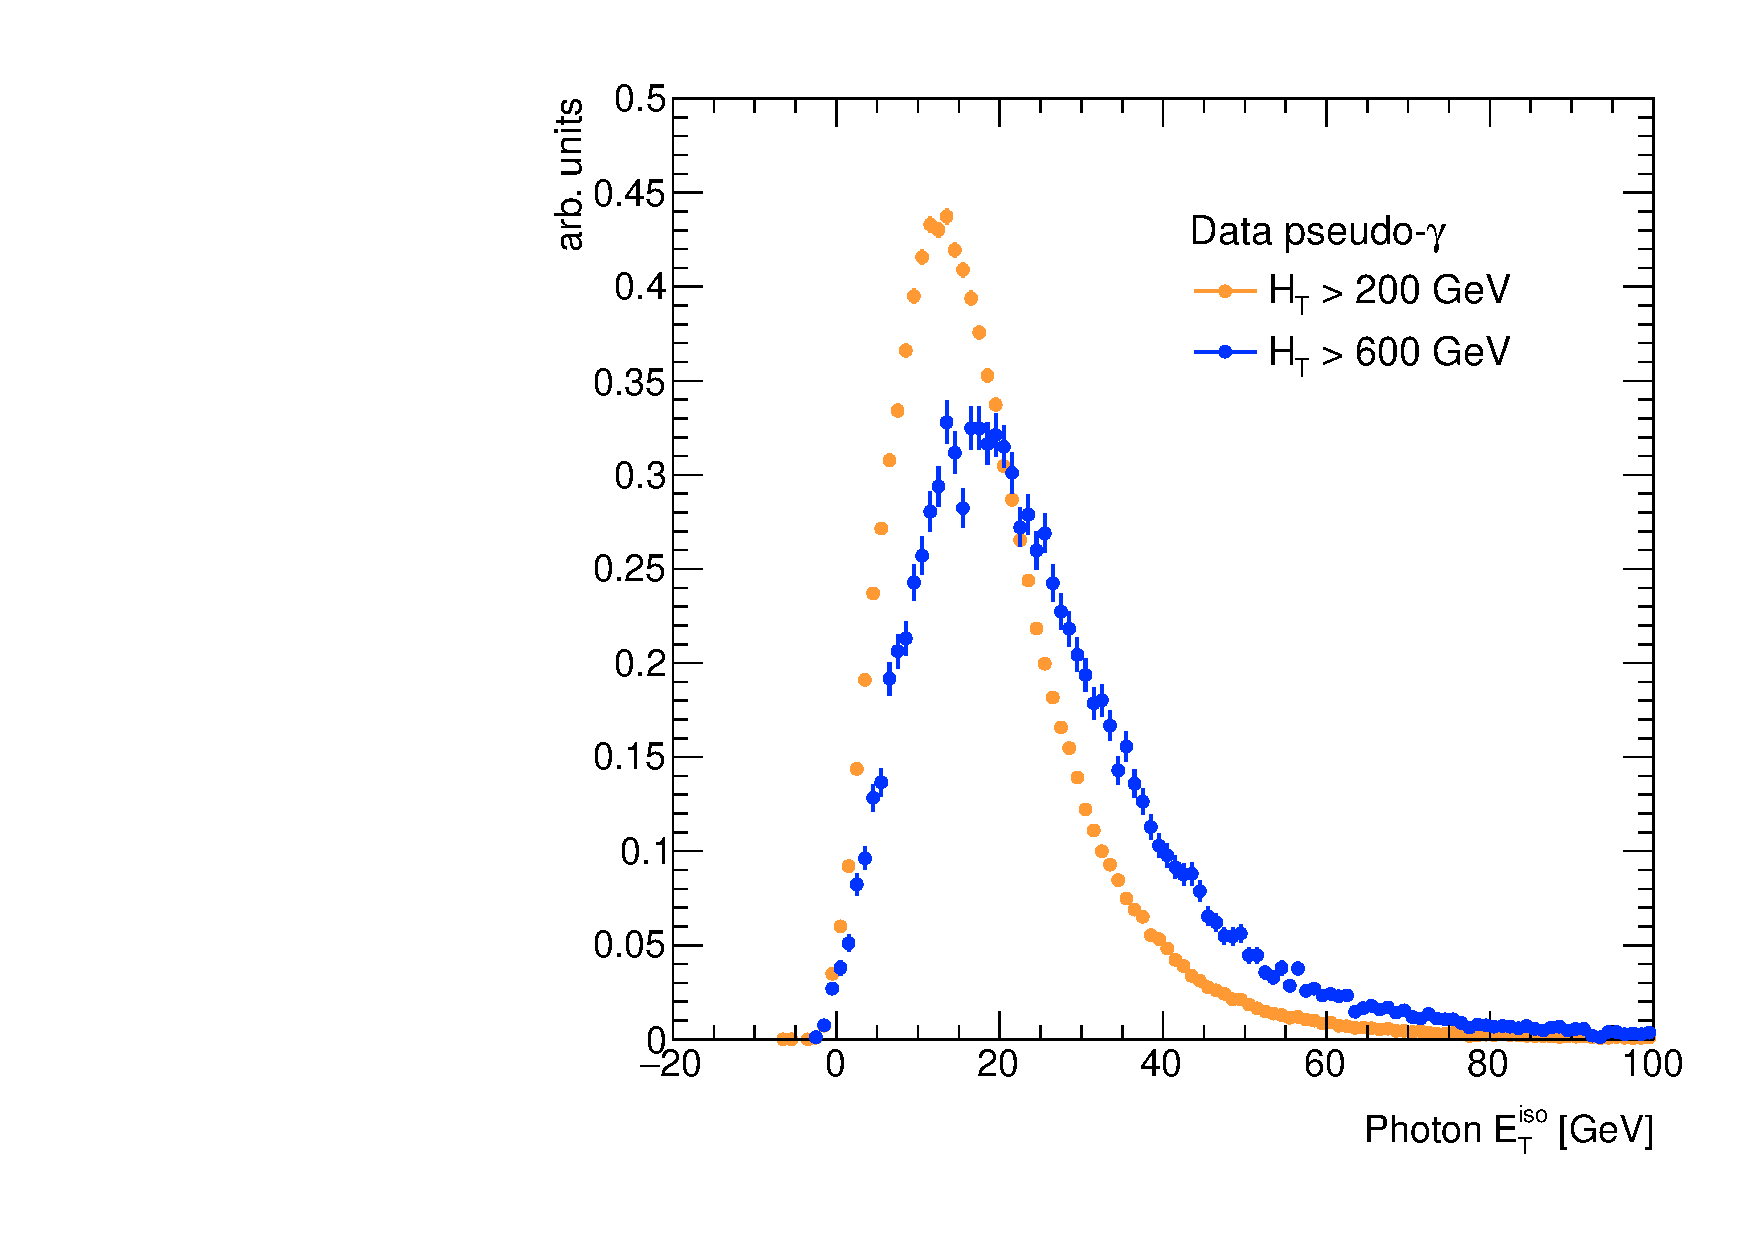
\includegraphics[width=0.49\textwidth]{figures/bkg_pseudo_data_SR_VR_l}
  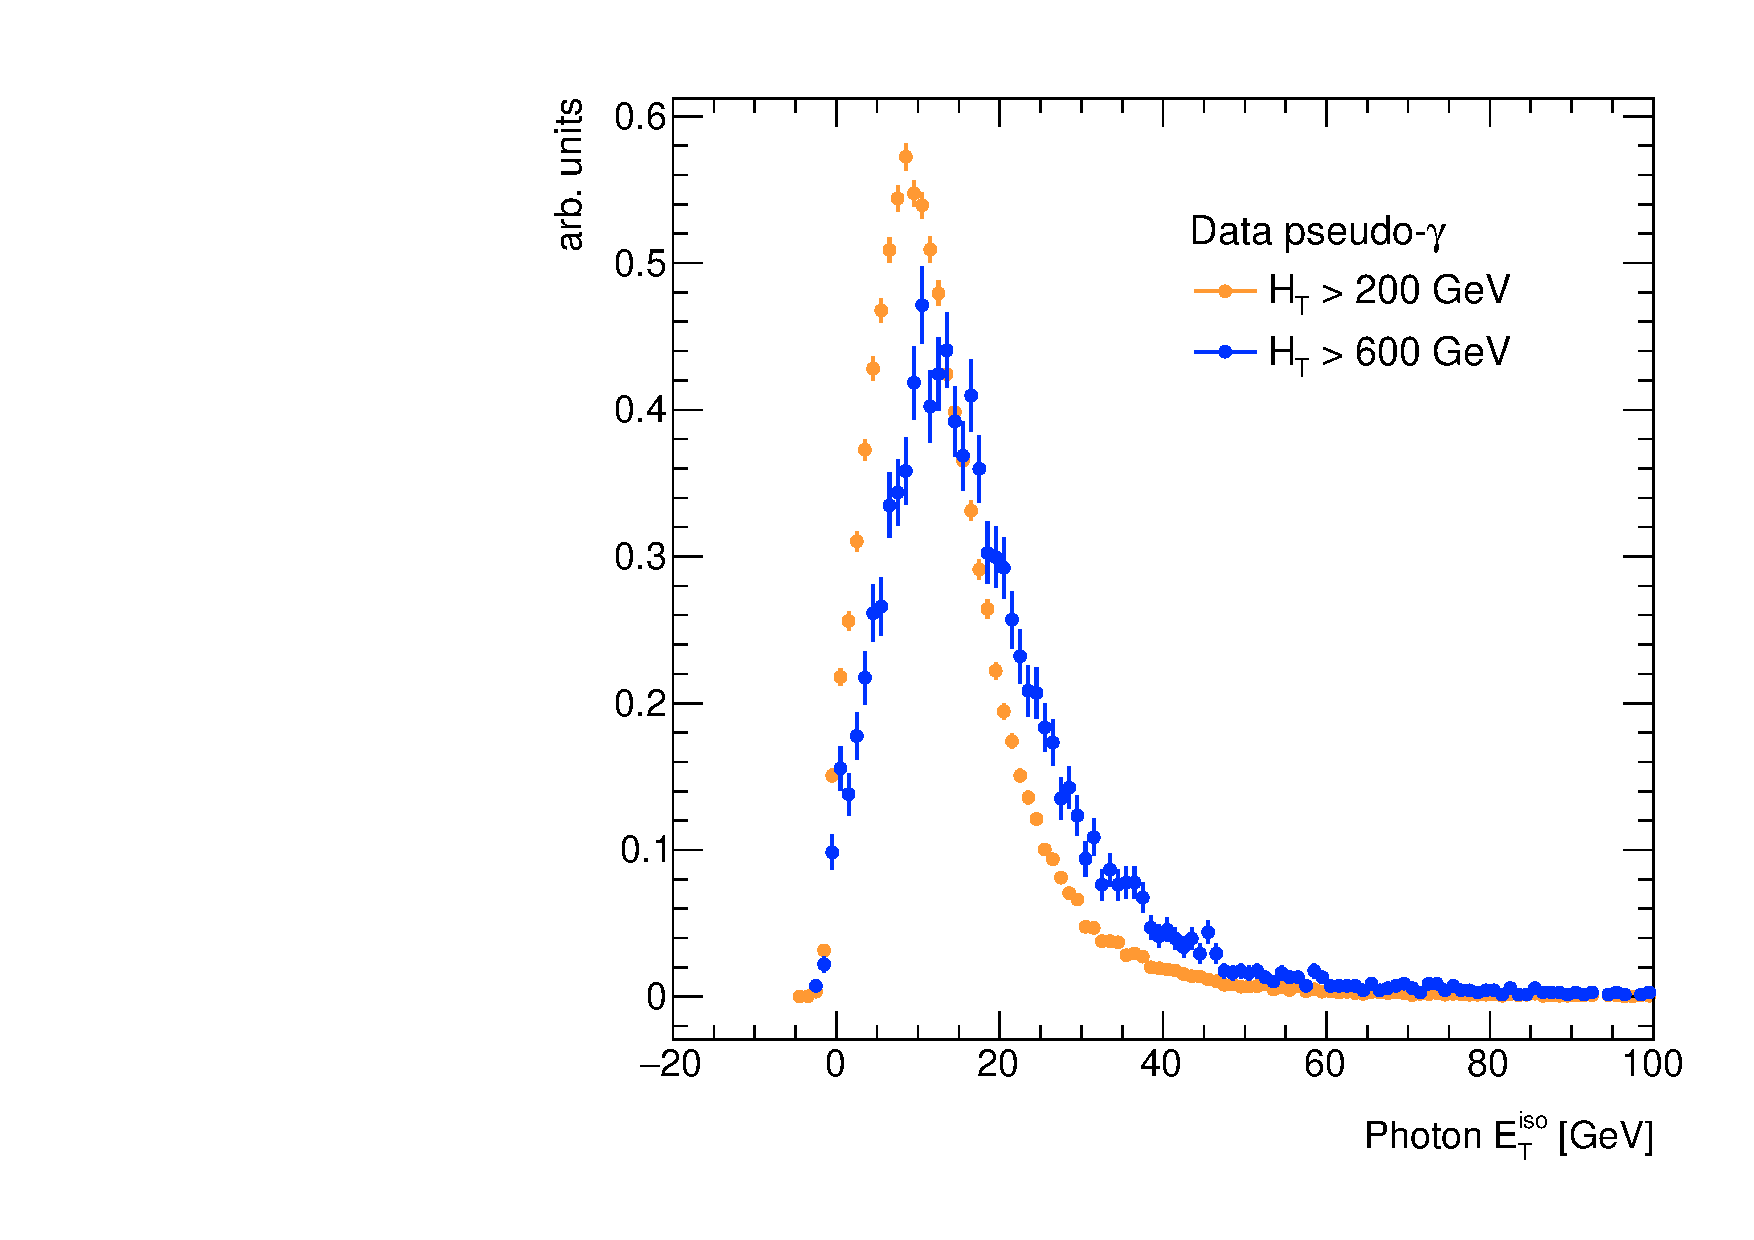
\includegraphics[width=0.49\textwidth]{figures/bkg_pseudo_data_SR_VR_lp}

  \caption{Distribución de la energía de aislamiento para pseudo-fotones \emph{loose-non-tight} (izquierda) y \emph{loose'-non-tight} (derecha),
    luego de la selección con un corte en $\HT>200 \gev$ y $\HT>600 \gev$.}
  \label{fig:jetfake_pseudo_data_LR_VR}

\end{figure}

Finalmente, se encuentra que la distribución de los pseudo-fotones está bien
descripta por una función \emph{Crystall-Ball}. La
distribución en datos y el ajuste puede verse en la \cref{fig:jetfake_sigbkg}.

%% The parametrized template is used in the combined
%% fit to tight photon data to derive the jet fake rate.

%% \begin{figure}[h]
%%   \begin{center}
%%   \includegraphics[width=0.49\textwidth]{iso_fit_bkg_wpars}
%%   \caption{Fit to the observed isolation template for  loose'-non-tight pseudo-photon data in the VR.}
%%   \end{center}
%%   \label{fig:jetfake_bkg_template_fit}
%% \end{figure}


\subsection{Ajuste combinado y estimación del fondo} \label{sec:jet_fake_results}

%% A template fit to both signal and background distributions is then used to model the shape of the photon isolation
%% for each contribution, as shown in \cref{fig:jetfake_sigbkg}, together with the fitted parameters.
%The corresponding $\chi^2$/dof are 2.4 and 8.8 for signal and background templates with 240 points.

A fin de modelar la forma de la energía de aislamiento de los fotones \emph{tight} en los datos,
se utiliza el modelo de señal y fondo descriptos en las secciones anteriores, como se puede
apreciar en la \cref{fig:jetfake_sigbkg}.
La distribución de {\etiso} para todos los eventos que pasan los criterios de
selección de la región relajada CRJ es ajustada a una combinación lineal de
los modelos de señal y fondo. El ajuste combinado y cada componente de la
distribución pueden verse en \cref{fig:jetfake_combfit}. Los parámetros son
inicializados con los valores extraídos de los ajustes individuales a la señal y
el fondo, y se los permite variar dentro de su incerteza

%As this fit is the source of the biggest systematic uncertainty the range of the parameters is then extend to two times the
%individual fit uncertainties to compute the systematic of the method.

Para estimar la incerteza sistemática, el ajuste combinado es realizado
sin ninguna limitación en los parámetros. La incerteza obtenida es del
50\% del valor de $f_{j\to\gamma}$, lo suficientemente grande para contener
cualquier potencial inexactitud en el modelado de la señal y el fondo.

%The fitted parameters for the signal, background and combined fits are tabulated in \Tab \ref{tab:jetfake_fit_pars}.
%% Los parametros estimados del ajuste combinado estan tabulados en la
%% \cref{tab:jetfake_fit_pars}.

El número de fotones total (N$_\text{total}$) y falsos
(N$_{j\to\gamma}$) esperados es obtenido
integrando las componentes de fondo y total del ajuste combinado sobre todo el
rango $\etiso<5\gev$, respectivamente:

\begin{itemize}
\item[] N$_{j\to\gamma}= 24143 \pm 56$

\item[] N$_\text{total} = 281813 \pm 586$
\end{itemize}

La fracción $f_{j\to \gamma}$ es obtenida simplemente como el cociente
en la \cref{eq:jfake_formula}:

\begin{itemize}
\item[] $f_{j\to\gamma} = 0.0857 \pm 0.0003 \stat \pm 0.04 \;\syst$
\end{itemize}

\begin{figure}[!htb]
  \centering

  \includegraphics[width=0.49\textwidth]{figures/iso_fit_sig_wpars}  \hfill
  \includegraphics[width=0.49\textwidth]{figures/iso_fit_bkg_wpars}

  \caption{Ajuste a las distribuciones de {\etiso} de señal
    (izquierda) y fondo (derecha) (derecha) en la región
    relajada CRJ.}
  \label{fig:jetfake_sigbkg}

\end{figure}

\begin{figure}[!htb]
  \centering

  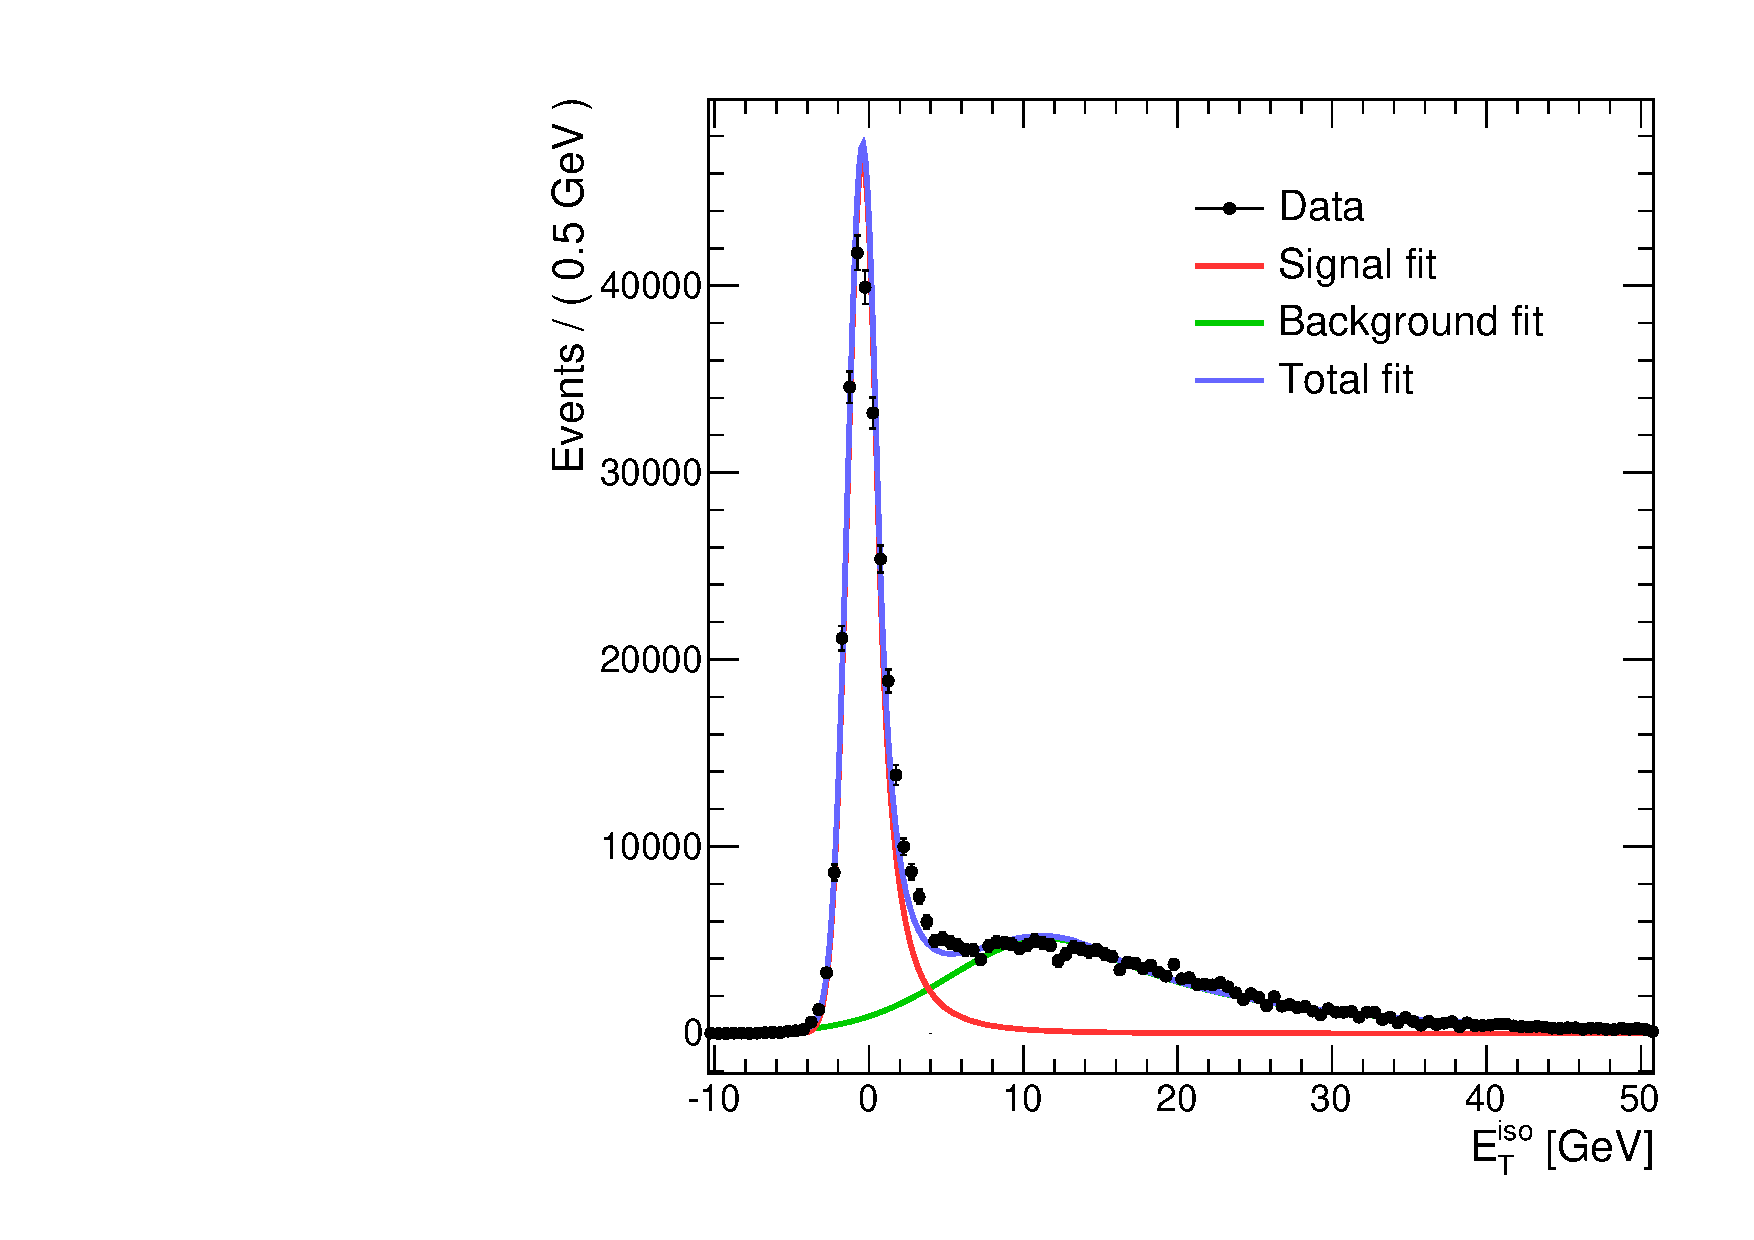
\includegraphics[width=0.49\textwidth]{figures/iso_fit_sarange}

  \caption{Ajuste combinado a la distribución de {\etiso}
    para los pseudo-fotones que pasan la selección de la región
    relajada CRJ (ver texto para detalles).}
  \label{fig:jetfake_combfit}

\end{figure}


El número de jets identificados erróneamente como fotones puede ser estimado
utilizando la fracción $f_{j\to\gam}$ como,

\begin{equation}\label{eq:njfakes}
  N_{j\to\gam} = f_{j\to\gam} \cdot N_\mathrm{tight}
\end{equation}

Para estimar la contribución en las SR, sin necesidad de utilizar el número de
eventos en las SR, lo que implicaría utilizar los datos en la region que se
utiliza para la búsqueda, se parametrizó este número como función de \met, como
se puede ver en \cref{fig:jetfake_nfakes_met}, utilizando una función
exponencial $N_{j\to\gam} = \exp(a+b \, \met)$ que luego se extrapola a la SR.
Los valores de $a$ y $b$ obtenidos del ajuste se muestran en la
\cref{tab:exppars}.

\begin{table}[!htbp]
  \centering
  \caption{Parámetros que resultan del ajuste a la distribución de $N_{j\to\gam}$ como función de {\met} con una función exponencial $\exp(a+b\, \met)$.}
  \begin{tabular}{crr}
    \hline
    Parámetro &  {\SRL} & {\SRH} \\
     \hline
     a & $3.87 \pm 1.25$  &  $1.80 \pm 0.98$ \\
     b &  $-0.054 \pm 0.018$  & $-0.047 \pm 0.014$ \\
     \hline
  \end{tabular}
  \label{tab:exppars}
\end{table}


La contaminación esperada de jets falsos en las SR se estima integrando la
parametrización de $N_{j\to\gam}$ sobre la región de {\met} de cada SR.

\begin{align}
  N_{j\to\gam}^\text{\SRL} &= \int_{200}^{\infty} N_\text{fakes}(\met) \, d\met = 0.01 \pm 0.02 \\
  N_{j\to\gam}^\text{\SRH} &= \int_{300}^{\infty} N_\text{fakes}(\met) \, d\met = 0.0001 \pm 0.0001
\end{align}

Debido a que las incertezas son de igual o mayor magnitud que los valores centrales,
se utilizaron los valores de estas como la estimación final en las SR.


\begin{figure}[!htbp]
  \centering
  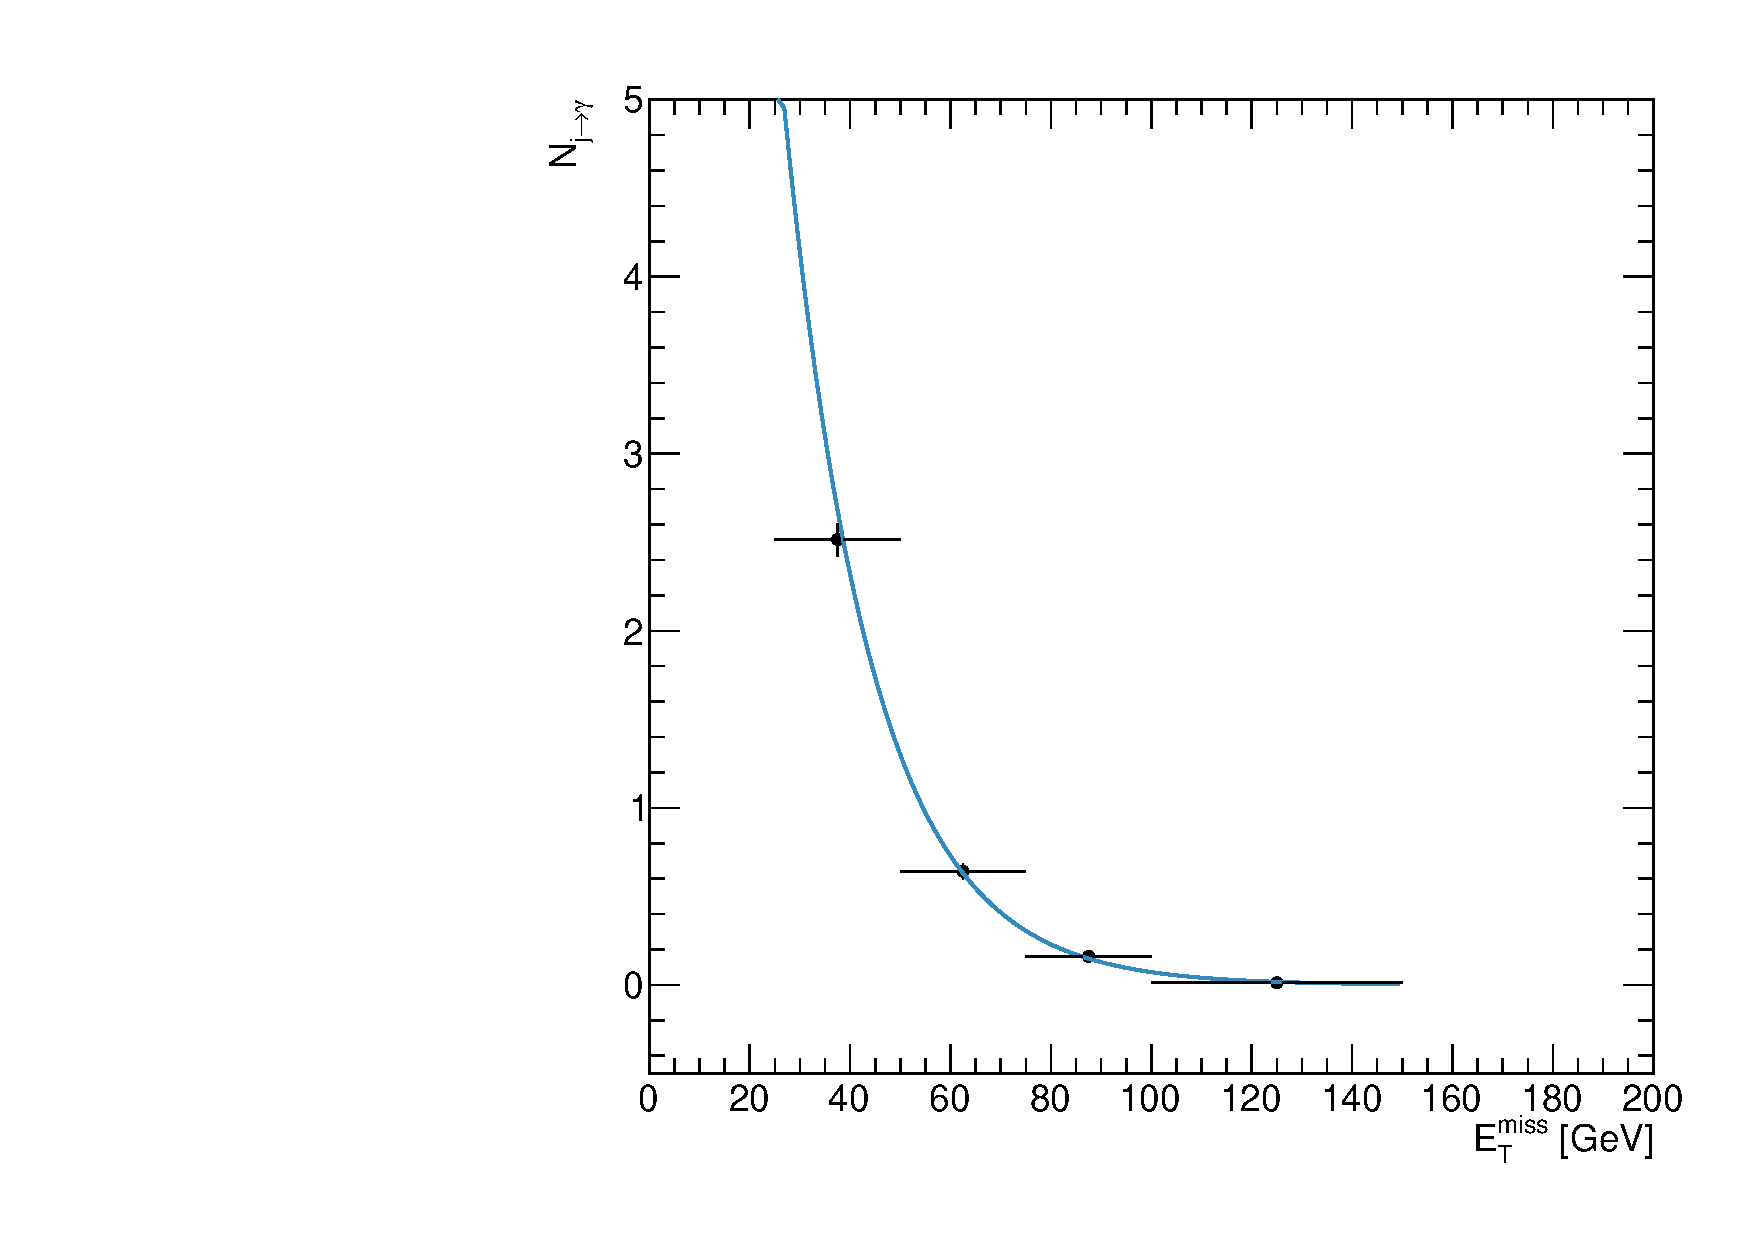
\includegraphics[width=0.49\textwidth]{nfakes_srl}  \hfill
  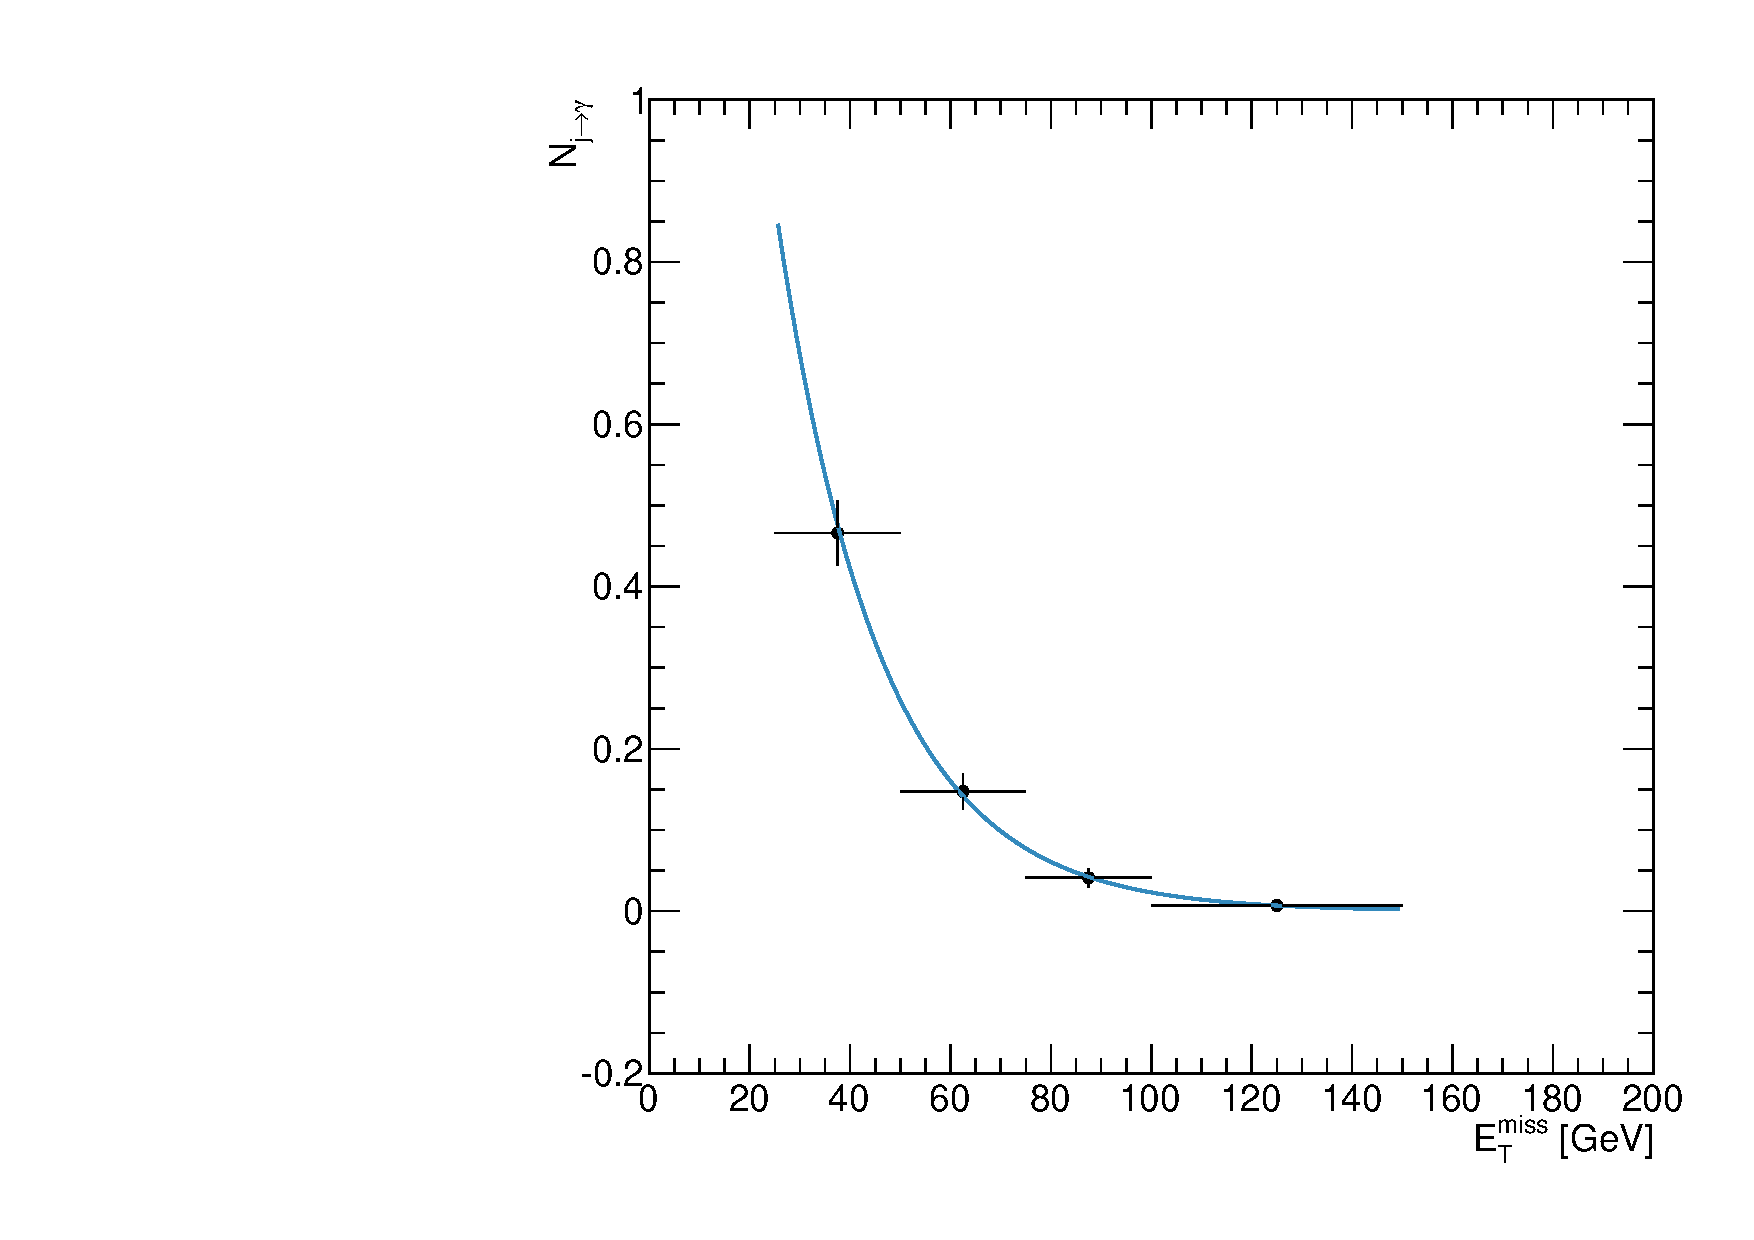
\includegraphics[width=0.49\textwidth]{nfakes_srh}
  \caption{Parametrización del número de jets mal identificados como
    función de {\met} para {\SRL} (izquierda) y {\SRH} (derecha).}
  \label{fig:jetfake_nfakes_met}
\end{figure}

El fondo de jets identificados como fotones es estimado similarmente en las
regiones de control y validación,
multiplicando el número de eventos observado en cada caso por el factor
$f_{j\to\gamma}$.


%% The final background contamination expected from jets faking photons is obtained by weighting the number of events observed in data,
%% after the otherwise full tight SR selections detailed in sec \ref{sec:signal_regions} (i.e. only the photon identification requirement is reversed).


%% Indeed, no pseudo-photon event was ultimately observed after all CRJ selections. This leads to a
%% j$\to\gamma$ background estimate of $<0.07$ events. Consistently, MC studies have shown this
%% background to be small in the high \MET\ and \HT\ regimes on the final SRs. As seen in \Tab \ref{tab:mc_events_sr_phtype}, the
%% MC predicts a jet fake contamination of $0.10\pm 0.04$ and $0.02 \pm 0.02$ event for SR2 and SR3, respectively.
%% This supports the findings in the data, agreeing within the uncertainties. The final jet fake background yield is estimated as $N^\text{SR}_\text{jfakes} = 0.0^{+0.1}_{-0.0}$, which accommodates an extra $+0.03$ uncertainty from the comparison of the MC-data predictions.
